% Version 2021
%

% Unidad 01. Tablero instrumentos

% Capítulo 1. Paneles de Instrumentos

% 1.1.       Introducción al estudio del instrumental.
% 1.2.       Clasificación de los Instrumentos.
% 1.3.       Distribución Normalizada del Instrumental en el Tablero
% 1.4.       Presentación en Pantalla Electrónica.

\chapter{Paneles de Instrumentos}
\label{chap:U01.paneles.instrumentos}


\section{Introducci\'on al estudio del instrumental}
\label{sec:01.01.introduccion.estudio.instrumental}

\begin{tcolorbox}{\bf Instrumento:} 
  Del lat. instrumentum.\\
  m. Objeto fabricado, relativamente sencillo, con el que se puede realizar una actividad.\\
  {\tiny Fuente: Diccionario R.A.E.}
\end{tcolorbox}

Los \textcolor{blue}{\bf Instrumentos de Vuelo} pueden definirse como
	el conjunto de mecanismos y dispositivos que forman parte de una aeronave y 
	que posibilitan que un vuelo se lleve a cabo en condiciones seguras 
( Fuente: \url{https://definicion.de/instrumento/}).

Estos instrumentos deben permitir: 

    \begin{itemize}
    \item Permitir volar en condiciones de clim\'aticas desfavorables, 
	con escasa visibilidad y durante la noche
    \item Asegurar una operaci\'on segura y confiable
    \item Dar avisos tempranos sobre cualquier falla en los sistemas
      de la aeronave o partes de la misma, de forma que los pilotos
      puedan tomar una acci\'on inmediata

    \end{itemize}
    
%  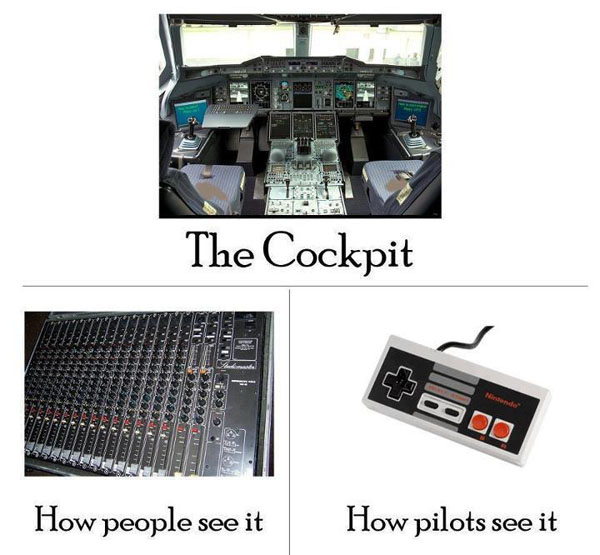
\includegraphics[width=\linewidth]{01.tablero.instrumentos/imagenes/1.1.introduccion/TheCockpit.jpg} \\
% {\tiny Fuente: \url{https://aviationhumor.net/flight-deck-cockpit-jokes-and-memes/}}

\Alerta{
    La habilidad de capturar y transmitir toda la informaci\'on que un piloto requiere, de forma segura y f\'acil de entender, ha sido un desaf\'io a trav\'es de la historia de la aviaci\'on, 
 \cite{FAA_Aviation_Maintenance_Technician_Handbook_Vol02}
}

En sus or\'igenes se equipaba a las aeronaves con pocos instrumentos debido a las cortas duraciones de los vuelos, sus costos y las complicaciones para el piloto en la interpretaci\'on de los mismos. \'este tipo de vuelo usualmente es conocido como \ac{VFR}.

% Hoy en d\'ia dicho concepto no est\'a vigente, entre otras razones por una mayor operatividad de las aeronaves, mayores tiempos de vuelo y la seguridad de sus tripulantes y pasajeros, por lo que este tipo de equipamiento se ha vuelto muy importante como as\'i tambi\'en sus costos. 

Los pilotos, cuya funci\'on es ser los ``\emph{cerebros}'' de la aeronave, deben tener conocimiento de todos los par\'ametros de la misma y los fen\'omenos que pueden ocurrir durante su operaci\'on, algunos de los cuales podr\'ian provocarle a sus sentidos indicaciones err\'oneas y, a veces, totalmente equivocadas. Es por ello que en el tiempo se han desarrollado todo tipo de instrumentos para asistir a los pilotos en sus funciones. 

La operaci\'on de una aeronave en condiciones atmosf\'ericas u horarias no comunes condujo a establecer las \ac{IFR}, para las cuales se necesita una capacitaci\'on y certificaci\'on adecuadas.

Las reglas de vuelo, tanto \ac{VFR} como \ac{IFR}  est\'an establecidas en Argentina por la \ac{ANAC} 
en la 
{RAAC 91} 
bajo el t\'itulo \emph{Reglas de vuelo por instrumentos (IFR)} 
y quien realiza un vuelo de \'este tipo debe poseer una 
\emph{Habilitación de Vuelo por Instrumentos} otorgada por la autoridad competente.

\begin{tcolorbox}
  La reglamentaci\'on de la ANAC se encuentra comprendida en las \ac{RAAC}, y pueden ser consultadas 
\href{http://www.anac.gov.ar/anac/web/index.php/2/120/normativa/raac-dnar}{en su sitio web}. 
En el mismo se encuentra la 
\href{http://www.anac.gov.ar/anac/web/uploads/normativa/raac/raac_vigentes/por_parte/parte-91-r-1-18.pdf}{RAAC Parte 91 ``{\it Reglas de vuelo y operación general }''}. 
A su vez tambi\'en  se dispone de la  
\href{http://www.anac.gov.ar/anac/web/uploads/normativa/raac/parte-91_subaprte1.pdf}{Subparte I - Aeronaves } 
y de la 
\href{http://www.anac.gov.ar/anac/web/uploads/normativa/raac/parte-91_subparte2.pdf}{Subparte II - Aviones grandes y turborreactores }.

\end{tcolorbox}

Es interesante observar la 
evoluci\'on en el tiempo de las cabinas de vuelo en donde se disponen los instrumentos de las aeronaves, ver Figura \ref {fig:01.evolucion.cabina}.


\begin{figure}[!htb]
  \centering
  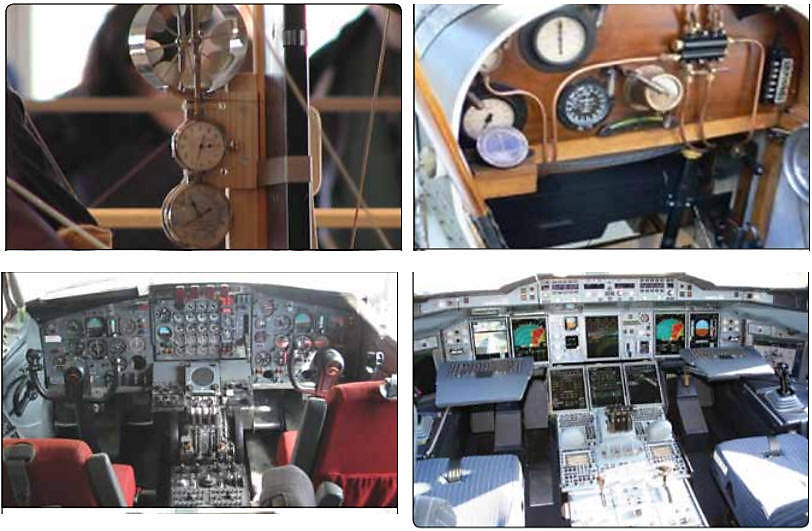
\includegraphics[height=0.6\linewidth, width=0.9\linewidth]{01.tablero.instrumentos/U01.imagenes/1.1.introduccion/evolucion_cabina.jpg} 

  \caption{{ Arriba izquierda: Wright Flyer, Arriba derecha: avi\'on primera guerra mundial, \\
      Abajo izquierda: Boeing 707 entre los '60 y '70, Abajo derecha: Airbus A380.}\\
    {\tiny Fuente:
      \url{https://www.waybuilder.net/free-ed/SkilledTrades/Aviation/AvAirframes/10AiInstrumt/10AiInstrumtFra.asp}}
  }
  \label{fig:01.evolucion.cabina}
\end{figure}

La evoluci\'on que ocurri\'o en el tiempo de los tableros de instrumentos de aeronaves puede apreciarse en la Figura \ref{fig:01.evolucion.tableros.instrumentos}

\begin{landscape}
  \begin{figure}[!htb]
    \centering
    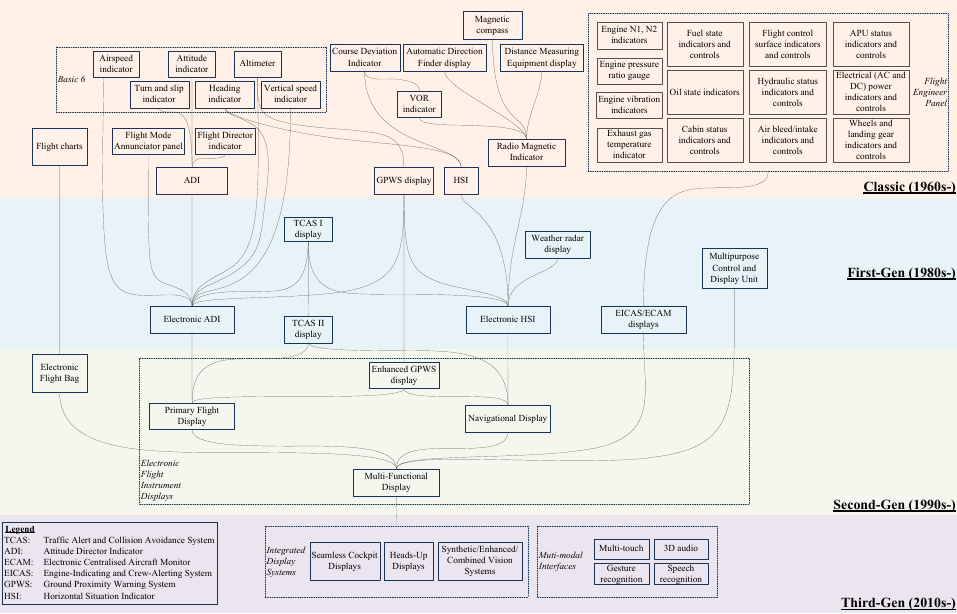
\includegraphics[width=\linewidth]{01.tablero.instrumentos/imagenes/1.1.introduccion/evolucion_cabina_00.png}

    \caption{Evoluci\'on de tableros de instrumentos en aeronaves
      \protect\cite{Lim2018AvionicsHI}.}
    \label{fig:01.evolucion.tableros.instrumentos}
  \end{figure}
\end{landscape}




\subsection{Ergonom\'ia}
\label{sec:ergonomia}

\begin{tcolorbox}
{\bf Ergonom\'ia:} 
\emph{Del griego.
  %	\griego{\'ergon}
  ''ergon'' (trabajo) y ``nom\'ia''
  % ( \griego{n\'omos}
  ``nomos'' (regla, ley),
  m\'as el sufijo ``ia'' (cualidad))}\\
1. f. Estudio de la adaptaci\'on de las m\'aquinas, muebles y utensilios a la persona que los emplea habitualmente, para lograr una mayor comodidad y eficacia.\\
2. f. Cualidad de ergon\'omico (adaptado a las condiciones del
usuario). \emph{El puesto de conducci\'on tiene buena ergonom\'ia.}

\begin{flushright}
  \textcolor{blue}{\it Fuente: Real Academia Espa\~nola }
\end{flushright}

\end{tcolorbox}

\emph{La Ergonom\'ia (o Factores Humanos) es la disciplina cient\'ifica relacionada con la comprensi\'on de las in\-te\-rac\-cio\-nes entre los seres humanos y los elementos de un sistema, y la profesi\'on que aplica teor\'ia, principios, datos y m\'etodos de dise\~no para optimizar el bienestar humano y todo el desempe\~no del sistema.
}
{\tiny Fuente: Asociaci\'on Internacional de Ergonom\'iía (IEA) \,
\url{https://www.iea.cc/whats/}}


\subsubsection{Ergonom\'ia Cognitiva}
\label{sec:01.ergonomia.cognitiva}

\begin{tcolorbox}
  ``{\it Se ocupa de los procesos mentales, tales como la
    percepci\'on, la memoria, el razonamiento y la respuesta motora,
    que afectan a las interacciones entre los seres humanos y otros
    elementos de un sistema. Los temas relevantes incluyen carga de
    trabajo mental, la toma de decisiones, el rendimiento experto, la
    interacci\'on persona-computadora, la fiabilidad humana, el
    estr\'es laboral y la forma como estos pueden estar relacionados
    con el dise\~no de los sistemas humanos. La ergonom\'ia cognitiva
    estudia los procesos de cognición en el trabajo y ajustes
    operativos, a fin de optimizar el bienestar humano y el
    rendimiento del sistema. } `` \cite{Asociacion_int_ergonomia}
\end{tcolorbox}

El campo de la Ergonom\'ia Cognitiva surgi\'o predominantemente al final de la d\'ecada de 1970 con la llegada de la computadora personal y los nuevos desarrollos en los campos de la psicolog\'ia cognitiva y la inteligencia artificial. Se contrasta con la tradici\'on de la ergonom\'ia f\'isica porque ``\emph{la ergonom\'ia cognitiva es... la aplicaci\'on de la psicolog\'ia cognitiva al trabajo... para lograr la optimizaci\'on (entre la gente y su trabajo) ... con respecto a al bienestar y productividad.}'' \cite{ergonomia_cognitiva_long_john}.

\begin{tcolorbox}
  Mayores detalles sobre Ergonom\'ia Cognitiva pueden consultarse en \cite{van_der_Veer} 
\end{tcolorbox}

Un esquema del modelo de procesamiento de informaci\'on puede observarse en la Figura \ref{fig:01.modelo.de.procesamiento.informacion.humano}.

\begin{figure}[!htb]
  \centering
  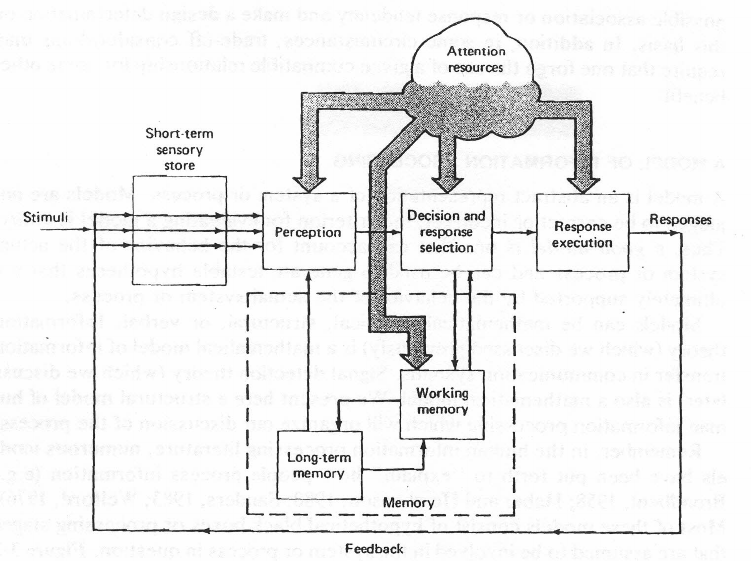
\includegraphics[width=0.8\linewidth]{01.tablero.instrumentos/U01.imagenes/1.1.introduccion/01-modelo_humano_procesamiento_informacion.png}
  
  \caption{Modelo  de procesamiento de informaci\'on humano \protect\cite{sanders1993human}}
\label{fig:01.modelo.de.procesamiento.informacion.humano}
\end{figure}

%{\tiny Fuente: Romosquera, \url{https://commons.wikimedia.org/wiki/File:Procesamiento_de_la_Informaci\%C3\%B3n.png}  }


\subsubsection{ Ergonom\'ia F\'isica}
\label{sec:ergonomia.fisica}

La Ergonom\'ia F\'isica se ocupa de las caracter\'isticas anat\'omicas, antropom\'etricas, fisiol\'ogicas y biomec\'anicas del usuario, en tanto que se relacionan con la actividad f\'isica.

Sus temas m\'as relevantes incluyen posturas de trabajo, sobreesfuerzo, manejo manual de materiales, movimientos repetitivos, Lesiones M\'usculo-Tendinosas (LMT) de origen laboral, dise\~no de puestos de trabajo, seguridad y salud ocupacional \cite{wiki_ergonomia_fisica}. 

En la Figura \ref{fig:01.dimensiones.estandard.cabina} puede apreciarse un estudio de la dimensiones interiores de una cabina y la ubicaci\'on de la persona dentro de la misma.


\begin{figure}[!htb]
  \centering
  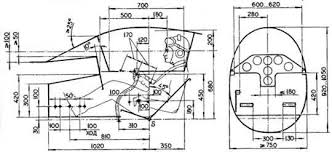
\includegraphics[width=0.9\textwidth]{01.tablero.instrumentos/U01.imagenes/1.1.introduccion/ergonomia_fisica.jpeg}
  
  \caption{Dimensiones estandar del interior de una cabina \protect\cite{cabina_ergonomia_fisica}}
\label{fig:01.dimensiones.estandard.cabina}
\end{figure}
%{\tiny Fuente: \url{https://www.ijsr.net/archive/v6i2/ART2017582.pdf}}




\subsubsection{Ergonom\'ia Visual}
\label{sec:01.ergonomia.visual}


La Ergonom\'ia Visual, como dominio dentro de la rama de ergonom\'ia, se centra en recomendaciones b\'asicas que deben cumplir aquellas personas que, en el desempe\~no de su actividad, emplean largas horas trabajando con pantallas y monitores. Estas recomendaciones incluyen aspectos como la separaci\'on entre el usuario y la pantalla, la necesidad de separar la vista del monitor repetidamente y centrarla en un punto lejano, o los beneficios de un parpadeo repetido que hidrate las capas corneales del ojo \cite{wiki_ergonomia_fisica}. 

\begin{center}
  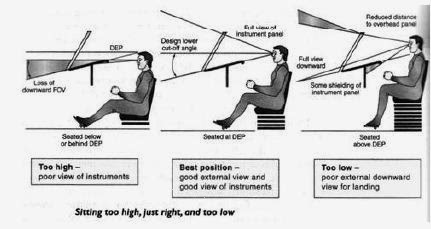
\includegraphics[width=0.7\textwidth]{01.tablero.instrumentos/U01.imagenes/1.1.introduccion/ergonomia_visual.jpg}
\end{center}
{\tiny Fuente: \url{http://avionics-system-design.blogspot.com/2013/12/ergonomics-of-aircraft-cockpit.html}}



\subsection{Formas de presentaci\'on de la informaci\'on}
\label{sec:formas.presentacion.informacion}

En vuelo, una aeronave y su tripulación forman un bucle de sistema ``{\it ser humano-máquina}'' que, según el tamaño y el tipo de la aeronave, puede ser bastante simple o muy complejo, ver Figura \ref{fig:01.bucle.ser.humano.maquina}. 
La función de la tripulaci\'on dentro de este bucle es la de controlador y el alcance de su función se rige por la simplicidad o no de la máquina como un todo integrado. 
Por ejemplo, al volar manualmente un avión e iniciar los ajustes a los sistemas esenciales se dice que la función del controlador es completamente activa. Si, por el contrario, el vuelo de un avión y los ajustes a los sistemas esenciales son automáticos, entonces la función del controlador pasa a ser de monitoreo, con la posibilidad de volver a la función activa en caso de falla de los sistemas.


\begin{figure}[!htb]
  \centering
  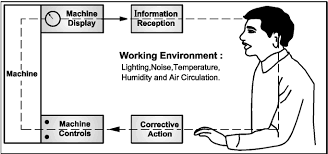
\includegraphics[width=0.5\textwidth]{01.tablero.instrumentos/U01.imagenes/1.1.introduccion/01-bucle_hbre_maquina.png}
  
  \caption{Bucle ser humano-m\'aquina \protect\cite{cabina_ergonomia_fisica}}
\label{fig:01.bucle.ser.humano.maquina}
\end{figure}



Los instrumentos tienen un rol vital en el circuito de control ya que son el medio de comunicar datos entre los sistemas y el controlador. Por lo tanto, para que un responsable del control  pueda obtener el máximo de calidad de control y, también para minimizar el esfuerzo mental en la interpretación de los datos, es necesario prestar la máxima atención al contenido y la forma de visualización de los datos.

Las formas más comunes de visualización de datos aplicadas a los instrumentos de aeronaves son:

\begin{enumerate}[a)]
\item \textbf{Cuantitativas}, en las que la cantidad variable que se mide
  se presenta en términos de un valor numérico y por la posición
  relativa de un puntero o índice, y
\item \textbf{Cualitativas}, en en el que la
  información se presenta en forma simbólica o pictórica.
\end{enumerate}

  \begin{itemize}
  \item {\bf Presentaciones cuantitativas:} ver Figura \ref{fig:01.presentaciones.cuantitativas}.
    \begin{itemize}
      \item Escala circular, es un m\'etodo cl\'asico de presentaci\'on de informaci\'on en forma cuantitativa. La escala del instrumento est\'a constitu\'ido por las correspondientes marcas de graduaci\'on. Su cantidad depende es una soluci\'on de compromiso seg\'un el tipo de informaci\'on a brindar: pocas marcas podr\'ian perder informaci\'on vital y producir errores de lectura, por el contrario una cantidad excesiva de marcas sobrecargar\'ia al operador y le insumir\'ia un tiempo excesivo de lectura. Los tama\~nos de las marcas son importantes y, usualmente, se numeran las marcas de cifras m\'as grandes las cuales presentan una longitud mayor. Es de suma importancia que el n\'umero de puntos posibles de medici\'on se elija cuidadosamente a fin de obtener lecturas r\'apidas y precisas.

El espaciado de las marcas 

      \begin{itemize}
         \item Escala lineal
         \item Escala no lineal (cuadr\'atica, logar\'itmica)
      \end{itemize}
       \item Escala longitudinal
       \item Presentaci\'on digital
    \end{itemize}
  \item {\bf Presentaciones cualitativas:} la información se presenta en forma simbólica o pictórica para mostrar la condición de un sistema como por ejemplo si el valor de una salida está aumentando o disminuyendo, el movimiento de un componente, etc. 

%En la Figura xx se muestran dos ejemplos típicos. El sincroscopio en (a) se utiliza junto con un rev./min. sistema indicador de una aeronave que tiene una disposición múltiple de motores de tipo hélice, y sus punteros, que simbolizan las hélices, solo giran para mostrar las diferencias de velocidad entre motores. La pantalla, que se muestra en (b), es un buen ejemplo de una que indica el movimiento de componentes; en este caso, superficies de control de vuelo, flaps de aterrizaje y deflectores de aire. El instrumento contiene diecisiete mecanismos eléctricos separados, que al ser accionados por transmisores, colocan elementos indicadores simbólicos de modo que aparezcan en varios ángulos detrás de las aberturas en el dial principal.



  \item {\bf Presentaciones directoras} ver Figura \ref{fig:01.presentaciones.directoras},  son aquellas que están asociadas principalmente con la actitud de vuelo y los datos de navegación.  Es importante presentarlos de una manera que indique al piloto qué movimientos de control debe hacer para corregir cualquier desviación de una trayectoria de vuelo deseada o para hacer que la aeronave realice una maniobra específica. 
En el desarrollo de este tipo de visualización debe existir una estrecha relación entre la dirección de los movimientos de control y el puntero del instrumento o elemento indicador de tipo simbólico, esto es los movimientos deben ser en el sentido "natural" para que el piloto pueda obedecer las ``\emph{directivas}'' o ``\emph{demandas}'' de la pantalla.
 
 \end{itemize}

  \begin{figure}[!htb]
    \centering
\subfigure[Escala circular cuantitativa \protect\cite{pallett1992aircraft}]{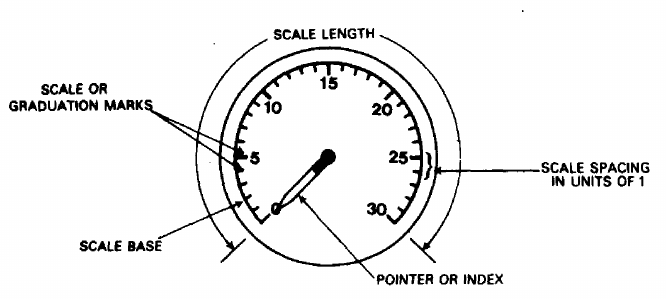
\includegraphics[width=0.45\textwidth]{01.tablero.instrumentos/U01.imagenes/1.2.clasificacion.instrumentos/escala_circular_cuantitativa.png}    }
\subfigure[a)Lineal, b) Ley cuadr\'atica , c) Ley logaritmica \protect\cite{pallett1992aircraft}]{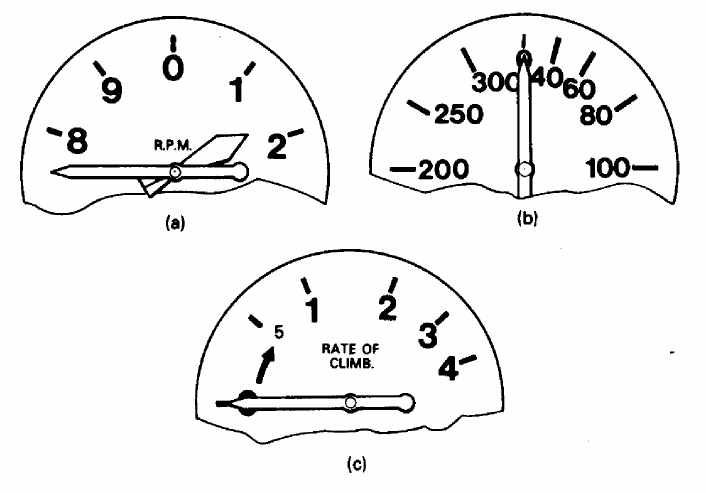
\includegraphics[width=0.45\textwidth]{01.tablero.instrumentos/U01.imagenes/1.2.clasificacion.instrumentos/escala_circular_lineal_no_lineal.png}}

\subfigure[a)Escalas conc\'entricas, (b) escalas fijas y giratorias, (c) escala com\'un tres agujas, (d) aguja dividida \protect\cite{pallett1992aircraft}]{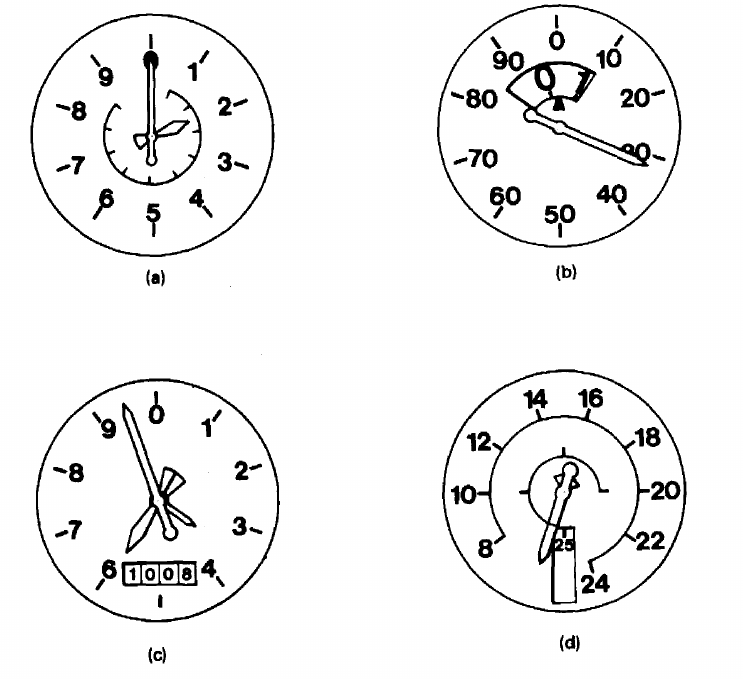
\includegraphics[width=0.45\textwidth]{01.tablero.instrumentos/U01.imagenes/1.2.clasificacion.instrumentos/escala_gran_alcance.png}}
\subfigure[Escala longitudinal \protect\cite{pallett1992aircraft}]{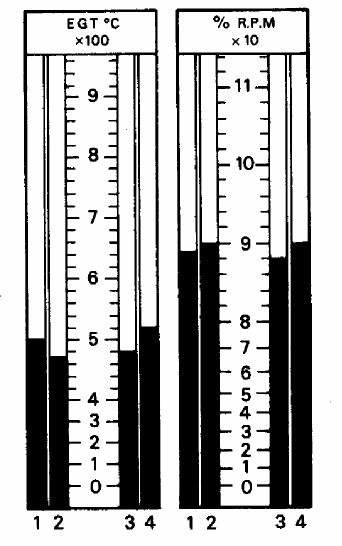
\includegraphics[width=0.35\textwidth]{01.tablero.instrumentos/U01.imagenes/1.2.clasificacion.instrumentos/longitudinal.png}}

    \caption{Presentaciones cuantitativas}
    \label{fig:01.presentaciones.cuantitativas}
  \end{figure}

  \begin{figure}[!htb]
    \centering
        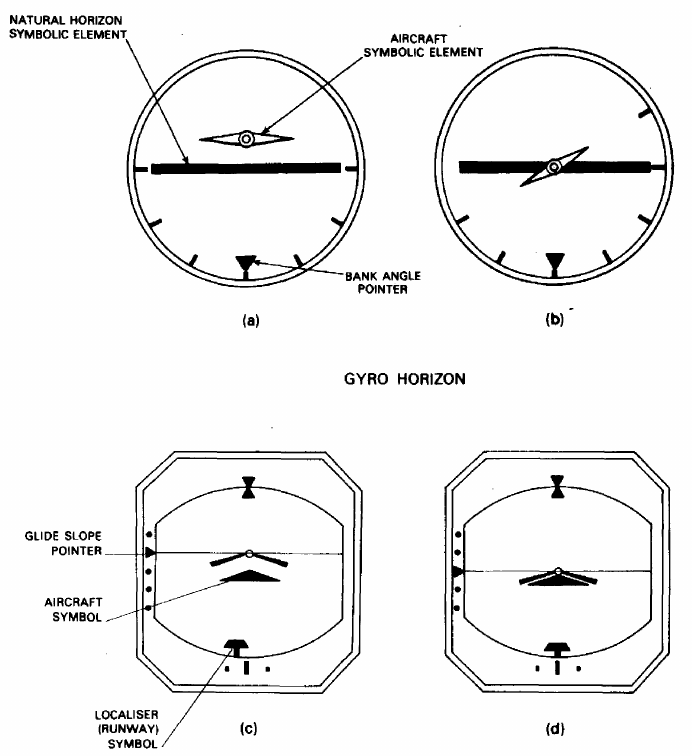
\includegraphics[width=0.75\textwidth]{01.tablero.instrumentos/U01.imagenes/1.2.clasificacion.instrumentos/director.png}
    \caption{Presentaciones directoras \protect\cite{pallett1992aircraft}}
    \label{fig:01.presentaciones.directoras}
  \end{figure}


%     \begin{tabular}{ccc}
%     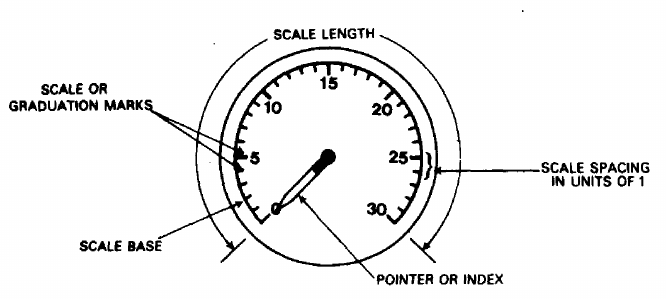
\includegraphics[width=0.45\textwidth]{01.tablero.instrumentos/U01.imagenes/1.2.clasificacion.instrumentos/escala_circular_cuantitativa.png} & \hspace{3mm}
% &     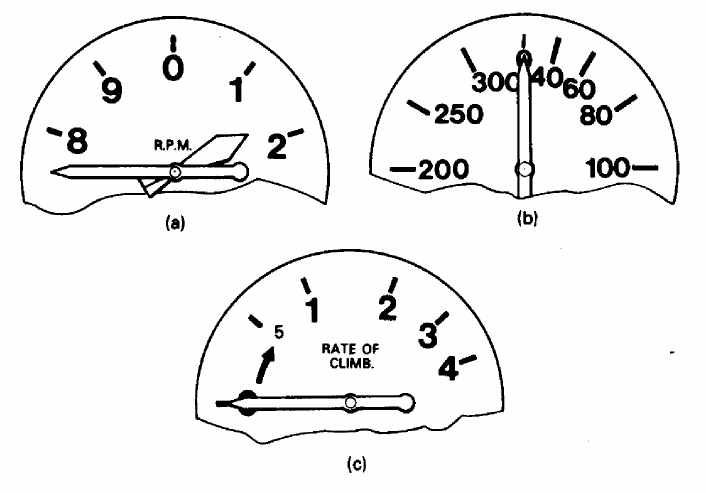
\includegraphics[width=0.45\textwidth]{01.tablero.instrumentos/U01.imagenes/1.2.clasificacion.instrumentos/escala_circular_lineal_no_lineal.png}
% \\
% 	Escala circular cuantitativa & 
% & \parbox{0.45\textwidth}{a) Lineal, b) ley cuadr\'atica, \\c) ley logaritmica}
% \\
%   \end{tabular}

% {\tiny Referencia: \cite{pallett1992aircraft}}

%   \begin{tabular}{ccc}
%     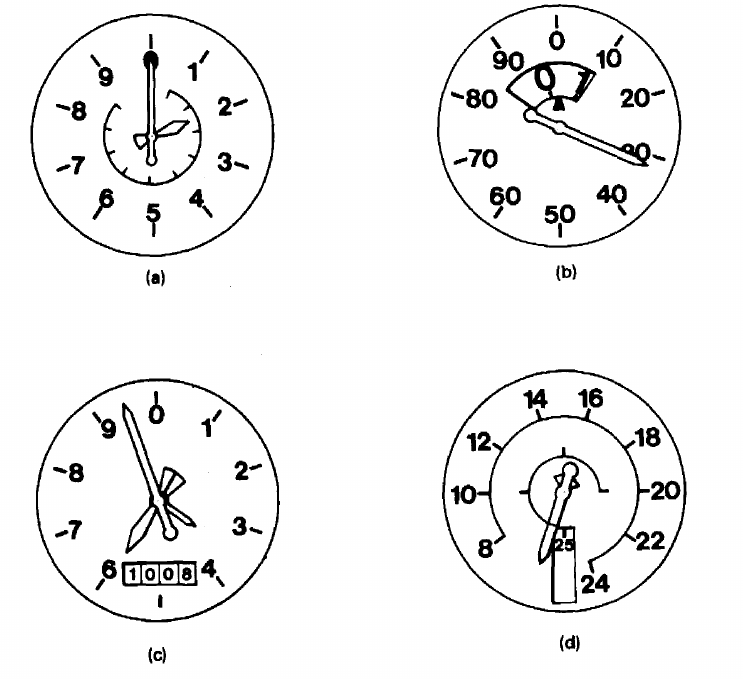
\includegraphics[width=0.45\textwidth]{01.tablero.instrumentos/U01.imagenes/1.2.clasificacion.instrumentos/escala_gran_alcance.png} & \hspace{3mm}
% &     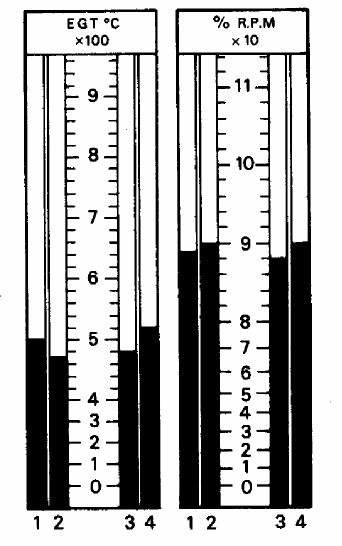
\includegraphics[width=0.35\textwidth]{01.tablero.instrumentos/U01.imagenes/1.2.clasificacion.instrumentos/longitudinal.png}
% \\
% \parbox{0.45\textwidth}{\small a)Escalas conc\'entricas, (b) escalas fijas y giratorias, (c) escala com\'un tres agujas, (d) aguja dividida}
% &
% & {\small Escala longitudinal}
% \\
%   \end{tabular}
% {\tiny Referencia: \cite{pallett1992aircraft}}


%   \begin{tabular}{ccc}
%     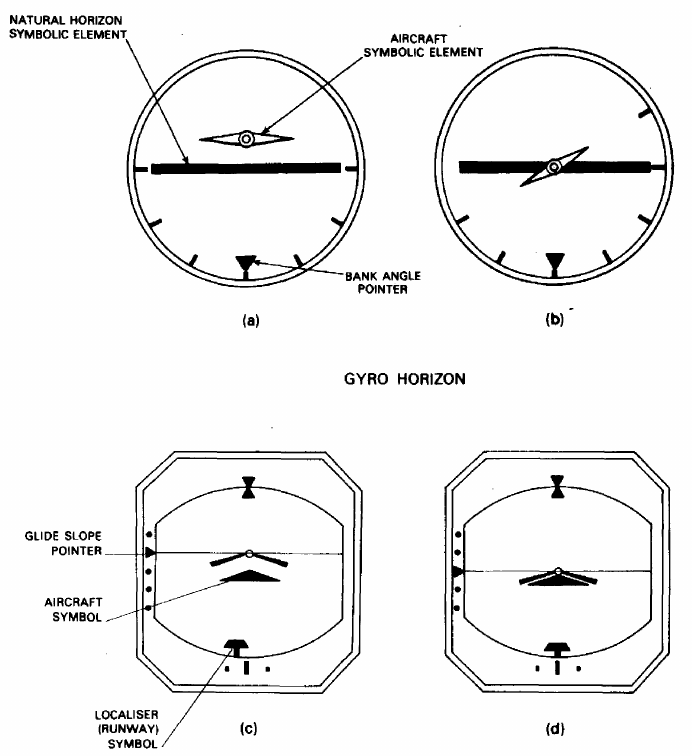
\includegraphics[width=0.45\textwidth]{01.tablero.instrumentos/U01.imagenes/1.2.clasificacion.instrumentos/director.png} & \hspace{3mm}
% &     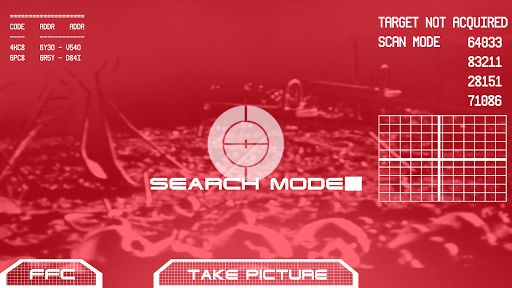
\includegraphics[width=0.5\textwidth]{01.tablero.instrumentos/U01.imagenes/1.2.clasificacion.instrumentos/terminator_hud.png}
% \\
% \parbox{0.45\textwidth}{Director de vuelo}
% &
% & Terminator Hud
% \\
%   \end{tabular}

% Head-Up Display
% Versión 2023
  
\subsubsection{Head Up Display }
\label{sec:HUD}
  
La simplicidad o no de presentaci\'on de la informaci\'on est\'a directamente involucrada a el número de instrumentos, por la cantidad de trabajo y secuencias de monitoreo de instrumentos que debe realizar un piloto durante las diversas fases del vuelo. En la fase crítica de aproximación y aterrizaje un piloto debe transferir su atención con mayor frecuencia de los instrumentos a las referencias fuera de la aeronave y viceversa. Un proceso de transición que lleva mucho tiempo y es fatigoso como resultado del constante reenfoque de los ojos.

Por lo tanto, se ha desarrollado un método para aliviar estos problemas en el que los datos de vuelo vitales se presentan al mismo nivel que la línea de visión del piloto cuando se ven referencias externas, es decir, cuando se mantiene una posición de ``{\it cabeza arriba}'' (head up). Los componentes de un sistema típico de visualización de esta forma, denominado \ac{HUD}, se pueden observar en la Figura \ref{fig:01.HUD} \cite{MikesFlightDeck}.

La cantidad de datos requeridos se rige por los requisitos de las diversas fases de vuelo y la función operativa de una aeronave, es decir, civil o militar, pero los  parámetros que se muestran son básicos. Los datos se transmiten desde una unidad de computadora de datos al tubo de rayos catódicos  cuya presentación es proyectada por el sistema óptico al infinito. La longitud, o rango, de las escalas está determinada por los requisitos operativos, pero normalmente solo cubren bandas estrechas de información de velocidad y altitud. Esto ayuda a reducir las marcas irrelevantes y el tiempo necesario para leer e interpretar. La  proyecci\'on óptica como una imagen simbólica compuesta sobre una placa reflectora transparente, o directamente sobre el parabrisas es lo que ve el piloto. %Se observará que la presentación de la actitud se asemeja a la de un horizonte giroscópico normal, y también que la velocidad y la altitud se presentan mediante marcadores que se registran contra escalas lineales horizontales y verticales. 

El HUD usa aplicaciones ópticas para agregar símbolos generados por computadora al campo de visión frontal del piloto, por esto se dice que es una clase de pantalla colimada, al parecer que las imágenes añadidas estan en el infinito óptico. Esto proporciona dos ventajas principales:

\begin{itemize}
\item Las imágenes permanecen alineadas con la vista exterior independientemente de cómo cambie el punto de vista del piloto.

\item El piloto no necesita volver a enfocar los ojos cuando cambia entre otro instrumento y la lectura de los datos del HUD. 
\end{itemize}

Esto significa que el sistema óptico es más complejo que un simple espejo parcialmente reflectante.

Una lente esférica, plano-convexa colimará una imagen, pero este enfoque tan simple tiene algunas deficiencias: introducirá distorsión geométrica en la imagen, no todos los colores estarán enfocados para la misma posición de la lente y cuando el centro de la imagen esté enfocado, los bordes de la imagen no lo estarán.

Se emplean lentes esféricos a pesar de estas limitaciones porque se pueden hacer formas esféricas con gran precisión con costos moderados. Las lentes asféricas fabricadas con una precisión similar pueden tener propiedades ópticas sustancialmente mejores, pero las complejidades de fabricación pueden hacer que el costo sea prohibitivo.

De todas maneras las lentes asféricas no son la respuesta final porque sólo pueden corregir distorsiones geométricas, puesto que las lentes, esféricas o no, funcionan refractando la luz y los ángulos de refracción cambian con la longitud de onda de ésta. Las lentes asféricas están sujetas a la aberración cromática al igual que las lentes esféricas.

El conjunto de óptica de colimación HUD consta de varias lentes simples. Al menos una de las lentes estará hecha de un material con un índice de refracción diferente. Las lentes individuales y los materiales de las lentes se eligen de modo que las aberraciones de las lentes individuales tiendan a cancelarse, dando como resultado una lente compuesta que tiene un rendimiento superior al de sus componentes.

Combinadores

Parcialmente reflectante

Los combinadores vienen en varias variedades. Uno simple es un espejo plano parcialmente plateado. Es viable pero pierde luz. Si tiene una relación de transmisión del 50\%, la mitad pasa y la otra mitad se refleja. Esto no es un problema para los datos de HUD, ya que la fuente de HUD se puede hacer más brillante. Sin embargo, es un problema con respecto a la visión delantera del piloto. La mitad de eso también se refleja. Puede jugar con la relación de transmisión para reducir la pérdida de visión hacia adelante, pero eso solo funciona hasta ahora.

Otra característica molesta de estos combinadores es la presencia de reflejos internos. La luz se reflejará en las superficies delantera y trasera. Los reflejos aparecen como imágenes fantasma.

Los reflejos internos se pueden minimizar utilizando un revestimiento antirreflectante en la superficie no reflectante del sustrato del espejo. El recubrimiento genera reflejos en sus superficies frontal y posterior. El grosor del recubrimiento se controla de modo que la reflexión de la superficie posterior esté desfasada con la reflexión de la superficie frontal. Al estar fuera de fase, se anulan entre sí. El índice de refracción se elige de manera que las dos reflexiones sean de la misma magnitud para asegurar la mejor cancelación. Los revestimientos antirreflectantes se ajustan a una sola longitud de onda de luz, pero dan resultados adecuados en una gama de colores.

Dicroico

Un combinador mejorado hace uso de un espejo dicroico. Esto es similar a un recubrimiento antirreflectante, pero se utilizan muchas capas y el grosor del recubrimiento se elige para mejorar el reflejo de una longitud de onda particular. Otras longitudes de onda pasan con atenuación mínima. Cuando se usa un espejo dicroico, una banda estrecha de colores se bloquea fuera de la vista frontal del piloto y se reemplaza por los datos del HUD. Debido a que el color de la pantalla HUD coincide con la característica dicroica, prácticamente toda la luz generada por HUD se dirige al piloto y solo se bloquea una pequeña cantidad de luz exterior. Un combinador dicroico también está sujeto a reflexiones internas. Se utiliza un revestimiento antirreflectante en la parte trasera del combinador para controlar esto.

Catadióptrico

El combinador no tiene que ser plano. Se puede usar un combinador curvo para implementar parte de toda la colimación. Esto generalmente se conoce como HUD catadióptrico. Catadióptrico se refiere a un sistema óptico que incorpora elementos reflectantes y refractivos. Una gran ventaja de las ópticas reflectantes es que no sufren aberración cromática. Al igual que las lentes, se fabrican más fácilmente en formas esféricas y, por lo tanto, también sufren de aberración esférica. Esto se puede corregir a través del diseño del sistema óptico tal como se corrige un sistema basado en lentes.

Holográfico

El término ``{\em HUD holográfico}'' puede recordar a una película de SciFi pero, lLa realidad es mucho simple. Un HUD holográfico simplemente usa un elemento óptico holográfico o HOE como combinador. Esta es una rejilla de difracción especializada que puede combinar y colimar. Los HOE pueden tener una longitud de onda muy específica para permitir que la cantidad máxima de luz del campo de visión delantero pase al piloto. Un HUD holográfico puede ofrecer un campo de visión más amplio para un peso dado que un HUD basado únicamente en lentes y/o espejos.


\begin{figure}[!htb]
  \centering
  \subfigure[Principio de funcionamiento del
  HUD ]{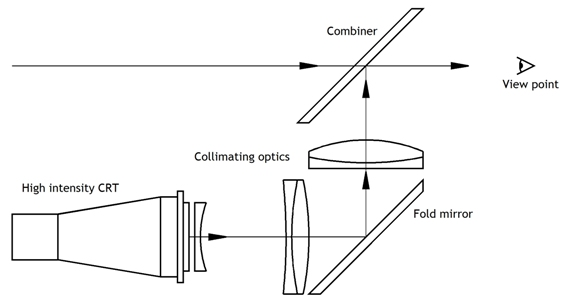
\includegraphics[width=0.45\textwidth]{01.tablero.instrumentos/U01.imagenes/1.2.clasificacion.instrumentos/hud_esquema.jpg}}
  \subfigure[Vista de un
  HUD]{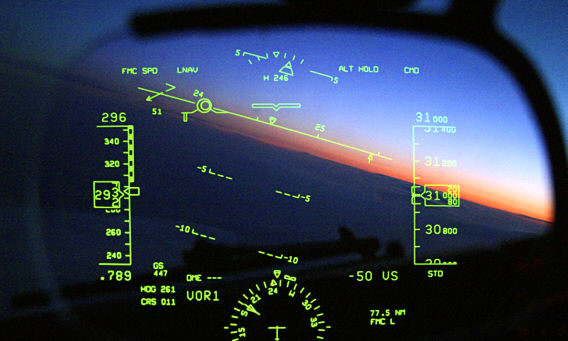
\includegraphics[width=0.45\textwidth]{01.tablero.instrumentos/U01.imagenes/1.2.clasificacion.instrumentos/hud.jpg}}
  
  \caption{HUD}
\label{fig:01.HUD}
\end{figure}


\begin{tcolorbox}
Un video interesante que cuenta la historia del HUD se encuentra en el siguiente link: 

  {
\includegraphics[width=0.1\textwidth]{01.tablero.instrumentos/U01.imagenes/Video.png}}\,
\href{https://www.youtube.com/watch?v=ypIbmfm7n8A}{The Evolution of the Head-Up Display}.
\vspace{3mm}


  Existen en el mercado peque\~nos \ac{HUD} para uso en aviaci\'on general como el provisto por la empresa Thales, el 
\href{https://www.thalesgroup.com/en/markets/aerospace/flight-deck-avionics-equipment-functions/topmax-wearable-hud-commercial-aircraft}{TopMax}.
\end{tcolorbox}


Tambi\'en se han desarrollado los \ac{EFVS} que son sistemas de visi\'on sint\'eticos, ver Figura \ref{fig:01.efvs}, 
 que proporciona una imagen de la escena y la muestra al piloto con el fin de proporcionar una imagen en la que la escena y los objetos en ella se pueden detectar mejor, esto es, un EFVS es un sistema que proporciona al piloto una imagen mejor que la visión humana sin ayuda. 

Los EFVS incluyen sensores de imágenes como una cámara a color, una cámara de infrarrojos o un radar y, normalmente una pantalla para el piloto, que puede ser una pantalla montada en la cabeza del mismo o una pantalla frontal. Un EFVS se puede combinar con un sistema de visión sintético para crear un sistema de visión combinado.
\href{https://www.youtube.com/watch?v=phbZintCgVA}{Video de un HUD/EFVS}.

\begin{figure}[!htb]
  \centering
\subfigure[EFVS]{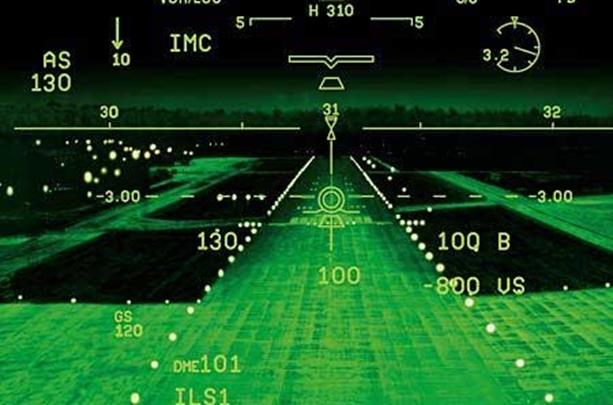
\includegraphics[width=0.45\textwidth]{01.tablero.instrumentos/U01.imagenes/1.2.clasificacion.instrumentos/EFVS_Photo.jpg}}
\subfigure[EFVS]{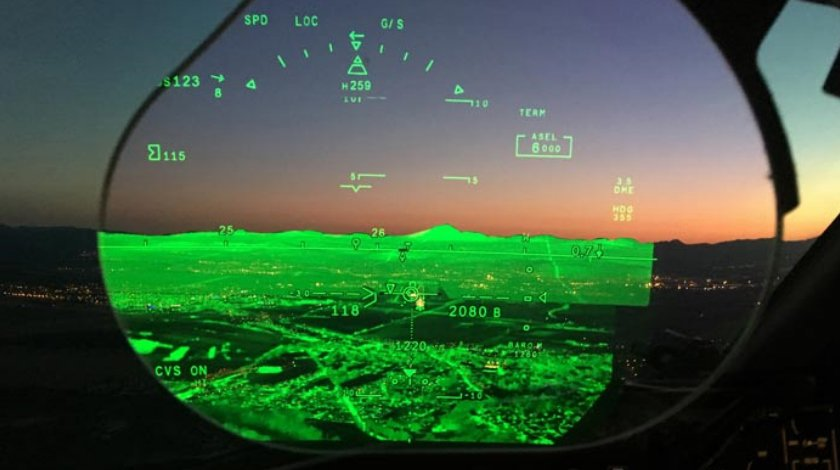
\includegraphics[width=0.45\textwidth]{01.tablero.instrumentos/U01.imagenes/1.2.clasificacion.instrumentos/efvs.jpg}}
  
  \caption{EFVS}
\label{fig:01.efvs}
\end{figure}







\section{Clasificaci\'on de los Instrumentos}
\label{sec:01.02.clasificacion.instrumentos}

Dentro de las distintas formas entre las cuales se podr\'ian clasificar los instrumentos de abordo, esto es por principio de funcionamiento, lectura directa, derivadores, integradores, a distancia, etc.; por lo anterior se puede clasificarlos seg\'un las magnitudes que miden. Seg\'un este criterio se los puede clasificar como:

\begin{itemize}
\item {\bf De Navegaci\'on:} que permiten determinar la posici\'on y el movimiento relativo de la aeronave con respecto a la Tierra.
\item {\bf De Actitud:} para conocer los \'angulos relativos que los ejes de la aeronave que pasan por su baricentro forman con la Tierra.
\item {\bf De Control:} entre los que se cuentan respecto al equipo propulsor y otros de equipos y sistemas varios de la aeronave.
\item {\bf Equipos Especiales:} tales como avisos de alarma, sistemas de seguridad, etc. 
\item {\bf Controles Autom\'aticos:} que reemplazan a los pilotos manteniendo cierta condici\'on de vuelo programada.
\end{itemize}

En la Figura \ref{fig:01.instrumentos.en.una.aeronave} tambi\'en puede observarse una clasificaci\'on de los instrumentos en una aeronave.

\begin{figure}[!htb]
  \centering
  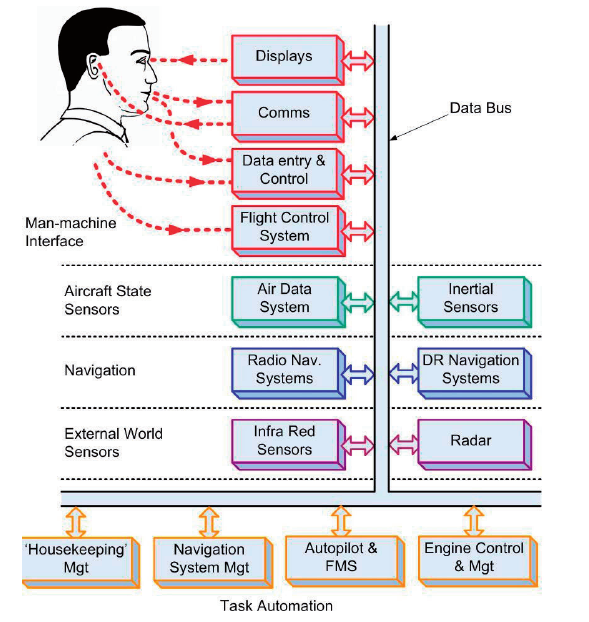
\includegraphics[width=0.9\textwidth]{01.tablero.instrumentos/U01.imagenes/1.2.clasificacion.instrumentos/tipos_instrumentos.png}  
  \caption{Instrumentos en una aeronave \protect\cite{Introduction_to_Avionics_Systems}}
  \label{fig:01.instrumentos.en.una.aeronave}
\end{figure}

%   Tambi\'en puede clasificarlos como se indica en la Tabla \ref{tab:01.clasificacion.instrumentos}.

% \begin{landscape}


% \begin{table}[!htb]
%   \centering
%   \caption{Clasificaci\'on de instrumentos}
%   \label{tab:01.clasificacion.instrumentos}

%   \begin{tabular}{cll} \hline \rowcolor{bubbles}
%     {\bf Tipo} & {\bf Instrumentos} & {\bf Descripci\'on / Requerimientos} \\ \hline

%    \parbox{0.15\textwidth}{\bf Sistema de \\ Pitot-Est\'atica}
%    &\parbox{0.30\textwidth}{
%         \begin{itemize}
%         \item Alt\'imetro
%         \item Veloc\'imetro
%         \item Indicador de Velocidad Vertical
%         \end{itemize}
%       }
%       &\parbox{0.65\textwidth}{ \scriptsize
%         \begin{itemize}
%         \item El sistema será hermético, excepto por los respiraderos a la atmósfera, y estará dispuesto de manera que la precisión de los instrumentos no se vea seriamente afectada por la velocidad, actitud o configuración de la aeronave; por humedad u otra materia extraña.

%         \item  El sistema debe estar provisto de una sonda de presión Pitot con calentamiento para evitar el mal funcionamiento debido a la formación de hielo.

%         \item Instalaci\'on de trampas de humedad para asegurar un drenaje positivo en todo el sistema.

%         \item  En aeronaves en las que se instalará un sistema alternativo o de emergencia, el sistema debe ser tan confiable como el primario y cualquier válvula selectora debe estar claramente marcada para indicar qué sistema está en uso.

%         \item  Las tuberías deben tener un diámetro interno tal que la diferenciade presión y la posibilidad de obstrucción por humedad se mantengan en un mínimo aceptable.

%         \item Cuando se utilicen ventilaciones estáticas, para evitar errores de guiñada, deberán estar situadas en lados opuestos de la aeronave y conectadas como un solo sistema. Cuando se prescriban sistemas duplicados, se proporcionará un segundo sistema similar.

%         \end{itemize}
%       } \\ \hline

%    \parbox{0.15\textwidth}{\bf Instrumentos giroscópicos}
%  	&
% 	&\parbox{0.65\textwidth}{ \scriptsize
% Los instrumentos giroscópicos pueden ser del tipo operado por vacío o eléctricamente, pero en todos los casos los instrumentos deben estar provistos de dos fuentes de energía independientes, un medio para seleccionar cualquiera de las fuentes de energía y un medio para indicar que la fuente de alimentación está funcionando satisfactoriamente. .

% La instalación y el sistema de suministro de energía deben ser tales que la falla de un instrumento, o del suministro de una fuente, o una falla en cualquier parte del sistema de suministro, no interfiera con el suministro adecuado de energía de la otra fuente.
% } \\ \hline
%     \end{tabular}
%   \end{table}


% \end{landscape}



%   \begin{tabular}{ccc}
%     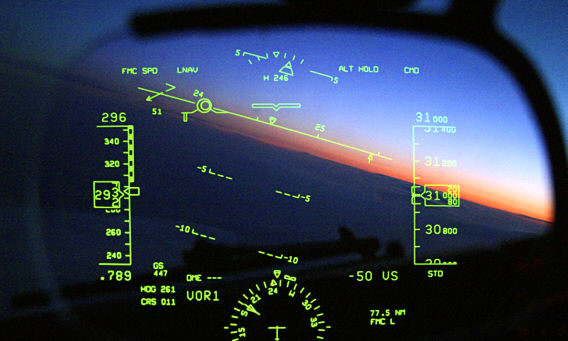
\includegraphics[width=0.45\textwidth]{01.tablero.instrumentos/U01.imagenes/1.2.clasificacion.instrumentos/hud.jpg} & \hspace{3mm}
% &     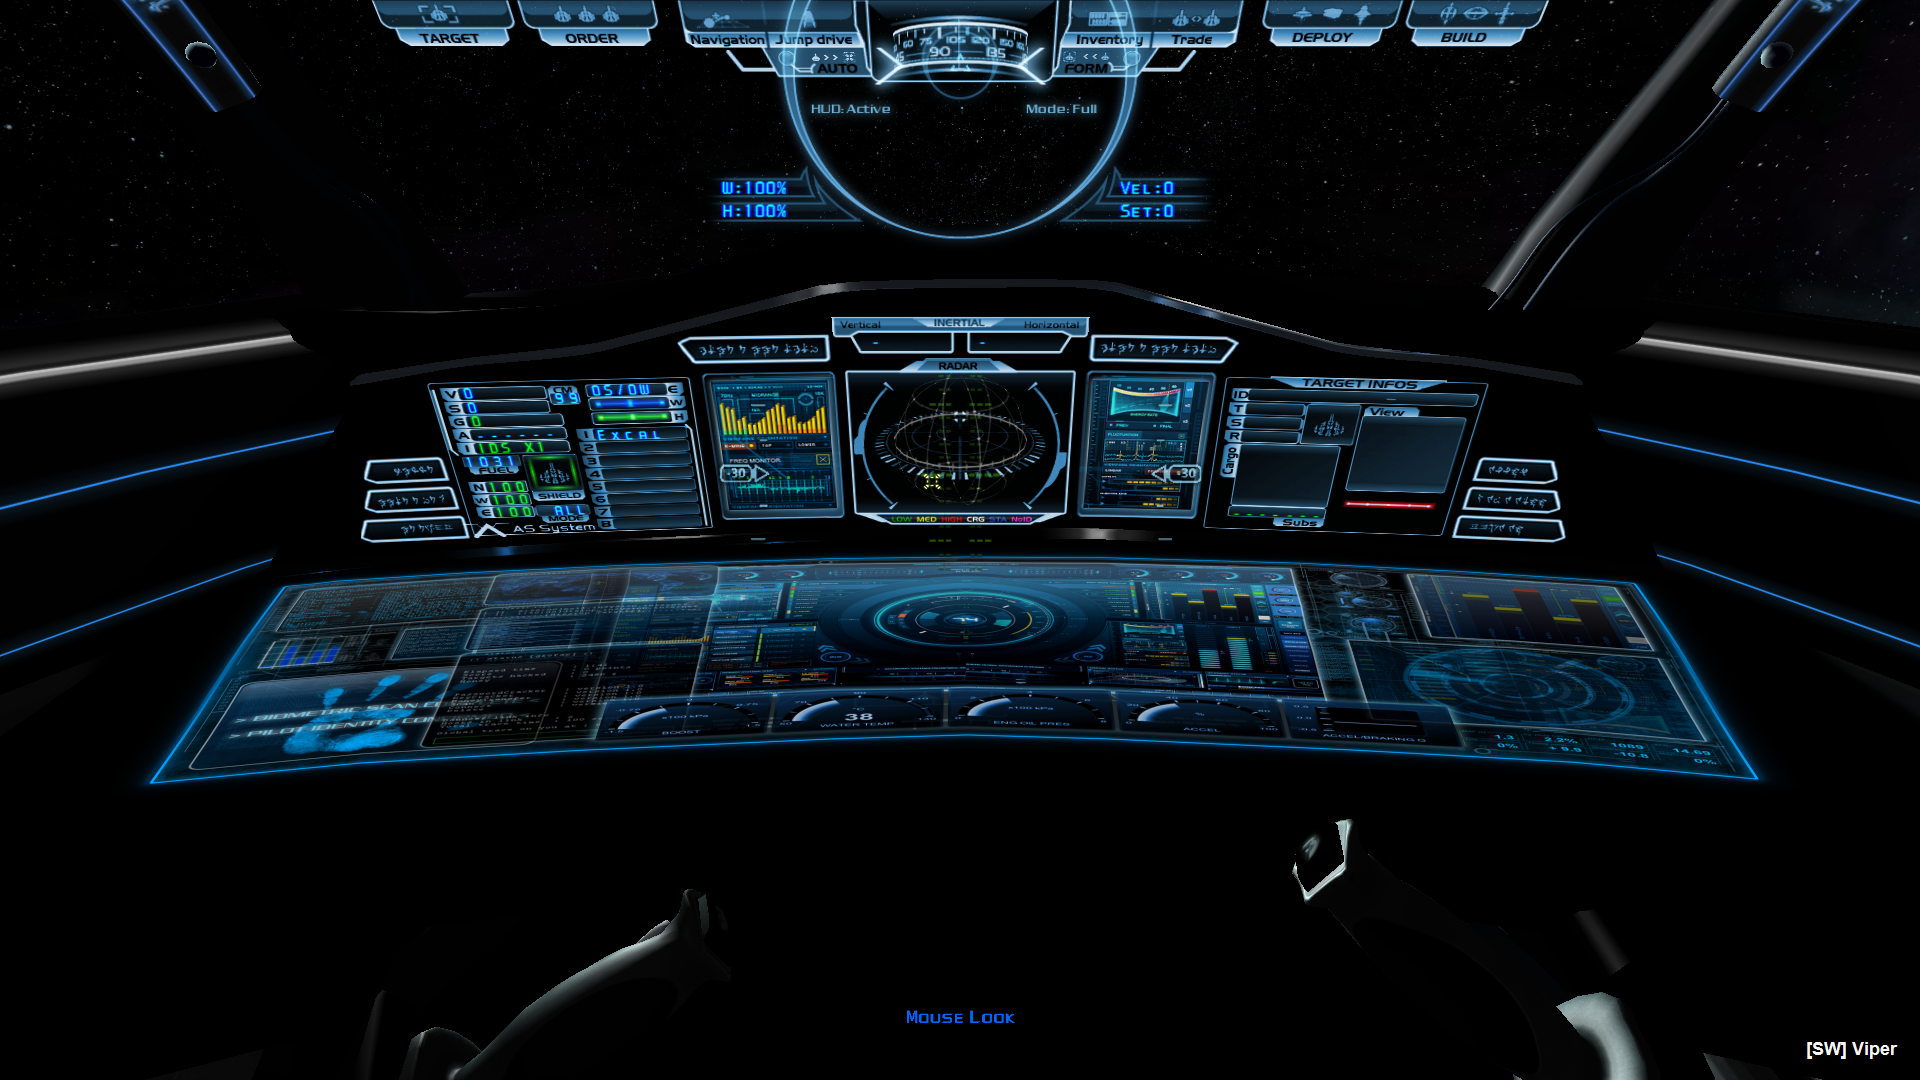
\includegraphics[width=0.5\textwidth]{01.tablero.instrumentos/U01.imagenes/1.2.clasificacion.instrumentos/viper_11.png}
% \\
% \parbox{0.45\textwidth}{Head Up Display}
% &
% & Hud futuro
% \\
%   \end{tabular}

  
% {
\includegraphics[width=0.1\textwidth]{01.tablero.instrumentos/U01.imagenes/Video.png}}\,
% Enhanced Flight Vision System \url{https://www.youtube.com/watch?v=DR9lyAM2YNE}
  


\section{Distribuci\'on Normalizada del Instrumental en el Tablero}
\label{sec:U01.03.distribucion.normalizada.instrumental}


En Argentina los requerimientos de instrumentos y equipos para aeronaves  civiles  motorizadas  con  Certificado de Aeronavegabilidad Estándar se encuentran contenidos en la \href{}{RAAC 91.205}, mencionada anteriormente.
En la misma se hace la distinci\'on entre:

\begin{itemize}
    \item Reglas de vuelo visual (VFR) diurno
    \item Reglas  de  vuelo  visual  (VFR)  nocturno
    \item Reglas de vuelo por instrumentos (IFR)
    \item Reglas de vuelo visual dentro del espacio aéreo controlado (VFR controlado)
\end{itemize}

En la Tabla \ref{tab:01.requerimientos.instrumentos.RAAC.91} se detallan los requerimientos anteriores.

% las CFAR se pueden encontrar en https://rgl.faa.gov/Regulatory_and_Guidance_Library/rgFAR.nsf/MainFrame?OpenFrameSet

A su vez se tienen las RAAC 23 y 25:

\begin{description}
\item[\href{https://www.anac.gov.ar/anac/web/uploads/upcg/raac/raac-23.pdf}{RAAC 23}] Estándares de aeronavegabilidad: aviones de categoría normal, utilitaria, acrobática y commuter.
\item[\href{https://www.anac.gov.ar/anac/web/uploads/upcg/raac/raac-25.pdf}{RAAC 25}]  Estándares de aeronavegabilidad: aviones de categoría transporte
\end{description}

En donde se hace mención de las 14 \ac{CFR} Part 23 y 25:

\begin{description}
\item[\href{https://www.law.cornell.edu/cfr/text/14/part-23/subpart-F}{14 \ac{CFR} Part 23 Sub Part F}]
\item[\href{https://www.law.cornell.edu/cfr/text/14/part-25/subpart-F}{14 \ac{CFR} Part 25 Sub Part F}] 
\end{description}

\newpage

  \begin{longtable}{m{0.25\textwidth}m{0.75\textwidth}}
    \caption{Requerimientos de instrumental seg\'un RAAC 91}
    \label{tab:01.requerimientos.instrumentos.RAAC.91} \\  \hline \rowcolor{bubbles}

      {\bf Reglas} & {\bf Instrumental requerido} \\ \hline \endfirsthead  \hline \rowcolor{bubbles}
      {\bf Reglas} & {\bf Instrumental requerido} \\ \hline \endhead

	\hline \endfoot  \hline \endlastfoot


      {\bf Reglas de vuelo visual (VFR) diurno}
      &
      {\scriptsize
        \begin{enumerate}
        \item Indicador de velocidad del aire.
        \item Un Baroaltímetro.
        \item Un reloj de precisión que indique las horas, minutos y
          segundos y que pueda mantener una exactitud de más o menos
          30 segundos durante un período de 24 horas.
        \item Indicador magnético de dirección.
        \item Tacómetro para cada motor.
        \item Medidor de presión (manómetro) de aceite, para cada
          motor que utilice circuito de presión de aceite.
        \item Medidor de temperatura (termómetro) para cada motor
          refrigerado por líquido.
        \item Medidor de temperatura de aceite para cada motor
          refrigerado por aire.
        \item Medidor de presión de admisión (Manifold) para cada
          motor alternativo capaz de mantener la potencia nominal de
          despegue desde el nivel del mar hasta una altitud
          establecida (tales como los motores con hélices de paso
          variable).
        \end{enumerate}
      } \\ \rowcolor{cyan!20}
\textbf{Reglas  de  vuelo  visual  (VFR)  nocturno}
& {\scriptsize
\begin{itemize}
	\item Todos los requeridos para VFR diurno
        \item Un indicador giroscópico de virajes.
\end{itemize}
}
\\ % \rowcolor{cyan!20}
\parbox{\linewidth}{\bf Reglas de vuelo por \\ instrumentos (IFR)}
& {\scriptsize
  \begin{itemize}
  \item Todos los requeridos para VFR diurno y nocturno
  \item Un sistema de radio comunicación que permita mantener una comunicación en ambos sentidos con las estaciones aeronáuticas en las frecuencias que prescriba la autoridad aeronáutica competente y el equipa-miento apropiado de navegación para las estaciones de tierra a ser utilizadas (VHF o HF). En caso de que no se disponga de equipo HF, las operaciones estarán sujetas a limitaciones especificadas en la RAAC 91.205.d.2.
  \item Un cronógrafo.
  \item Indicador giroscópico de velocidad de giro, excepto en las siguientes aeronaves:
    \begin{itemize}
    \item (i) Aviones con un tercer instrumento indicador de actitud
      que pueda medir todas las actitudes de vuelo a través de 360º de
      cabeceo y rolido y esté instalado de acuerdo con la Sección
      121.305 (j) de la Parte 121; y
    \item Helicópteros con un tercer
      instrumento indicador de actitud que pueda medir actitudes de
      vuelo entre +80º de cabeceo y +120º de rolido, esté instalado
      de acuerdo con la Sección 29.1303 (g) de la DNAR Parte 29.
    \end{itemize}
  \item Un Baroaltímetro sensitivo.
  \item Un Indicador de viraje y de inclinación lateral.
  \item Indicador giroscópico de inclinación lateral y cabeceo. (Horizonte artificial)
  \item Indicador giroscópico de dirección (girodireccional o equivalente).

{\it NOTA:Los  requerimientos  de:  indicador  de  viraje  y  de  inclinación  lateral,  indicador  de  actitud  de  vuelo  (horizonte  artificial),  e  indicador  de  rumbo  (giróscopo  direccional),  podrían  satisfacerse  mediante  combinaciones de instrumentos o sistemas integrados de dispositivos directores de vuelo, siempre que se conserven las garantías de que no ocurra una falla total, inherente a los tres instrumentos por separado.}

\item Medios para comprobar si es adecuada la fuente de energía que suministra energía a los instrumentos giroscópicos.
\item Un equipamiento aprobado de medición de distancia, \ac{DME}.
\item Un dispositivo que indique, en el compartimiento de la tripulación de vuelo, la temperatura exterior.
\item Un sistema indicador de la velocidad relativa con dispositivos que impidan su mal funcionamiento debido a condensación o a formación de hielo.
\item Un equipo \ac{VOR}.
\item Un equipo \ac{ADF} o equipo \ac{GNSS}.
\item Para los vuelos en que se proyecte aterrizar en condiciones meteorológicas de vuelo por instrumentos (IMC), el avión dispondrá de equipo que permita recibir las señales que sirvan de guía hasta un punto desde el cual pueda efectuarse un aterrizaje visual, \ac{ILS}.  

  \end{itemize}
}
\\  \rowcolor{cyan!20}
\parbox{\linewidth}{\bf Reglas de vuelo visual \\dentro del espacio aéreo\\ controlado\\ (VFR controlado)}
& {\scriptsize 
 Para vuelos VFR controlados dentro del espacio aéreo controlado, se requieren los siguientes equipamientos e instrumentos:
 \begin{itemize}
 \item Seg\'un las condiciones:
   \begin{itemize}
   \item Si el vuelo controlado es VFR – diurno, instrumentos y
     equipamientos especificados en Reglas de vuelo visual (VFR)
     diurno.
   \item Si el vuelo controlado es VFR – nocturno, instrumentos y
     equipamientos especificados en Reglas de vuelo visual (VFR)
     nocturno.
   \end{itemize}
 \item Un equipo VOR.
 \item Un equipo DME.
 \item Un variómetro.
 \item Un equipo ADF o equipo GNSS.
 \item Un  sistema  de  radiocomunicación  que  permita  mantener  una  comunicación  en  ambos  sentidos,  en  cualquier momento durante el vuelo con aquellas estaciones aeronáuticas en las frecuencias que prescriba la autoridad aeronáutica  competente  y  el  equipamiento  apropiado  de  navegación  para  las  estaciones  de  tierra  a  ser  utilizadas  (VHF  o HF).En  caso  de  que  no  se  disponga  de  equipo  HF,  las  operaciones  estarán  sujetas a las  limitaciones indicadas en RAAC 91.205.e.6.
 \item Un dispositivo que indique, en el compartimiento de la tripulación de vuelo, la temperatura exterior.
 \end{itemize}


}
\\

  \end{longtable}

%In 1937, the Royal Air Force selected six critical instruments to be installed in nearly all of its aircraft. Adopted by both commercial and general aviation aircraft manufacturers for decades thereafter, the arrangement became known as the “six pack.”

En 1937 la \ac{RAF} seleccion\'o seis instrumentos considerados esenciales en la cabina, conocidos como los ``\emph{basic six}'' (los seis b\'asicos), fue una distribuci\'on de instrumentos caracter\'istica de instrumentos en aviones brit\'anicos por los siguientes veinte a\~nos \cite{RAF_37}. Esta disposici\'on fu\'e adoptada tanto para aviaci\'on comercial como general por los fabricantes de aeronaves y es popularmente conocida como ``\emph{six pack}'''.
 
Esta distribuci\'on est\'a dividida en dos categor\'ias seg\'un se encuentren conectados al sistema de Pitot-Est\'atica o sean  Instrumentos Girosc\'opicos, en la Tabla \ref{tab:01.6-pack} puede observarse dicha clasificaci\'on y en la Figura \ref{fig:01-6-pack} su ubicaci\'on en el tablero de instrumentos.

\begin{figure}[!htb]
  \centering
  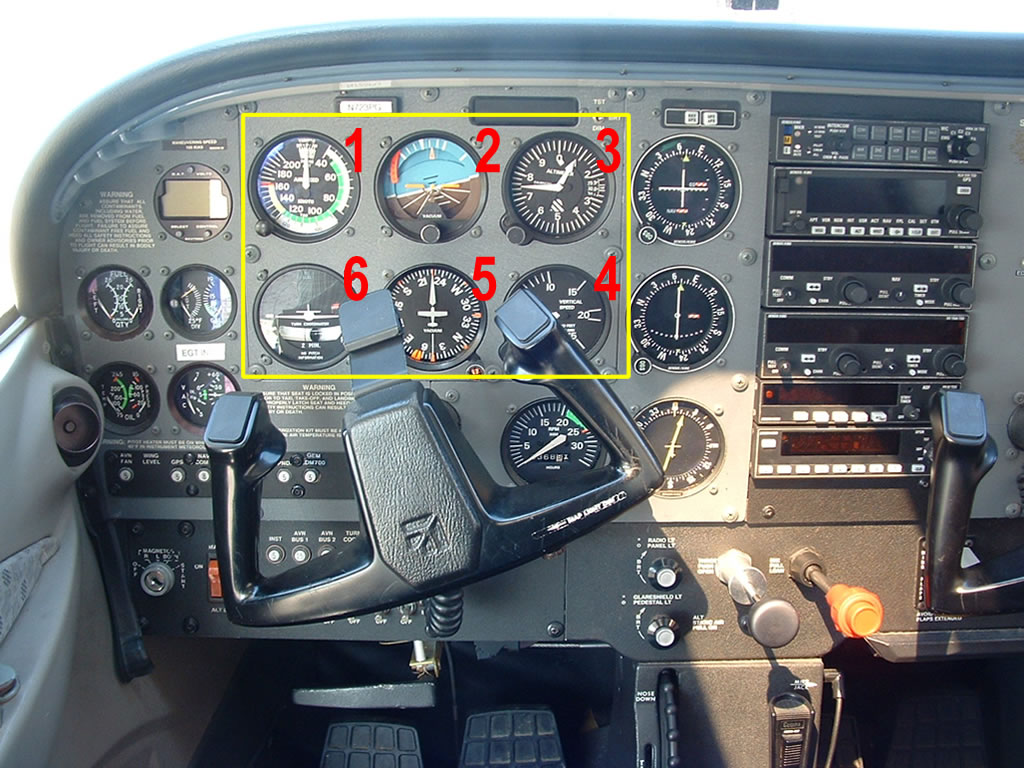
\includegraphics[width=0.8\linewidth]{01.tablero.instrumentos/imagenes/1.3.distribucion.normalizada.instrumental.en.tablero/01-Cessna-172-Instrument-Panel.jpg}
  \caption{Distribuci\'on de los basic six, \protect\cite{6-pack}}
  \label{fig:01-6-pack}
\end{figure}


\begin{table}[!htb]
  \centering
  \caption{Detalle de los instrumentos basic six}
  \label{tab:01.6-pack}
{\footnotesize
  \begin{tabular}{cm{0.35\textwidth}cc} \hline \rowcolor{azure} 
   \textcolor{white}{\bf Nro} & \centering \textcolor{white}{\bf Instrumento} 
	& \parbox{0.25\textwidth}{\textcolor{white}{\bf Instrumentos conectados \\al sistema de Pitot-Est\'atica}}
	& \parbox{0.15\textwidth}{\textcolor{white}{\bf Instrumentos girosc\'opicos}} \\ 
    {\bf 1} & Veloc\'imetro, \ac{ASI} & X & \\ \rowcolor{bubbles}
    {\bf 2 } & Indicador de Actitud, \ac{AI}, tambi\'en conocido como Horizonte Artificial & & X \\
{\bf 3} & Alt\'imetro & X & \\ \rowcolor{bubbles}
{\bf 4} & Indicador de Velocidad Vertical, \ac{VSI} & X & \\
{\bf 5} & Indicador de Rumbo, \ac{HI} & & X \\  \rowcolor{bubbles}
{\bf 6} & Indicador de Giro y Viraje, \ac{TC} & & X \\ \hline
  \end{tabular}
}
\end{table}

% Para el detalle de cada instrumento consultar https://www.mcico.com/resources/flight-instruments/six-pack-aircraft-instruments-explained

% y 

% https://learntofly.ca/six-pack-primary-flight-instruments/




\begin{tcolorbox}
  
Para observar distintos tipos de distribuci\'on de instrumental en cabinas de aeronaves puede hacerse una visita al 
Museo Nacional de la USAF, 
\href{https://www.nationalmuseum.af.mil/Visit/Virtual-Tour/Cockpit360/}{donde pueden apreciarse vistas de 360º de cabinas de diversas aeronaves}.

\href{https://pmflight.co.uk/free-airbus-cockpit-posters/}{Link para obtener vistas de la distribuci\'on de instrumentos en el tablero del Airbus A320 y el Boeing 737 NG.}


\end{tcolorbox}


\begin{figure}[!htb]
  \centering
    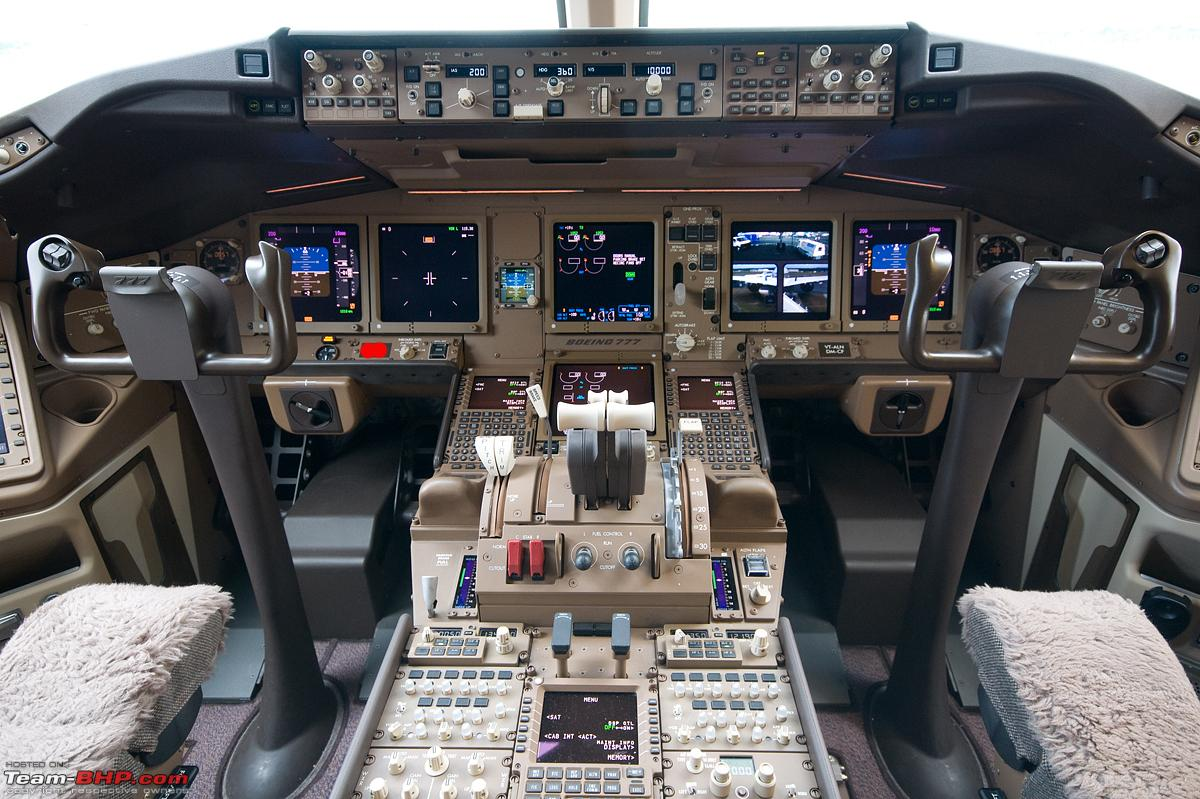
\includegraphics[width=0.95\textwidth]{01.tablero.instrumentos/U01.imagenes/1.2.distribucion.normalizada.instrumental.en.tablero/01-boeing777cockpit.jpg}

    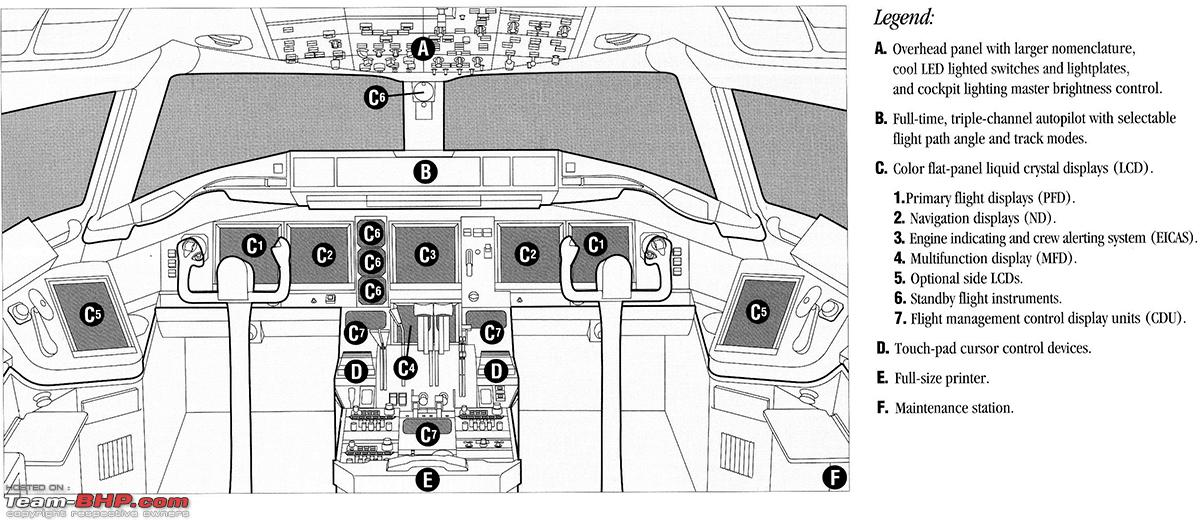
\includegraphics[width=0.95\textwidth]{01.tablero.instrumentos/U01.imagenes/1.2.distribucion.normalizada.instrumental.en.tablero/01-boeing777_cockpitlayout.jpg}   
  \caption{Cabina del Boeing 777 \protect\cite{Boeing777_cabina}}
  \label{fig:01.cabina.boeing.777}
\end{figure}



%https://pmflight.co.uk

\begin{figure}[!htb]
  \centering
    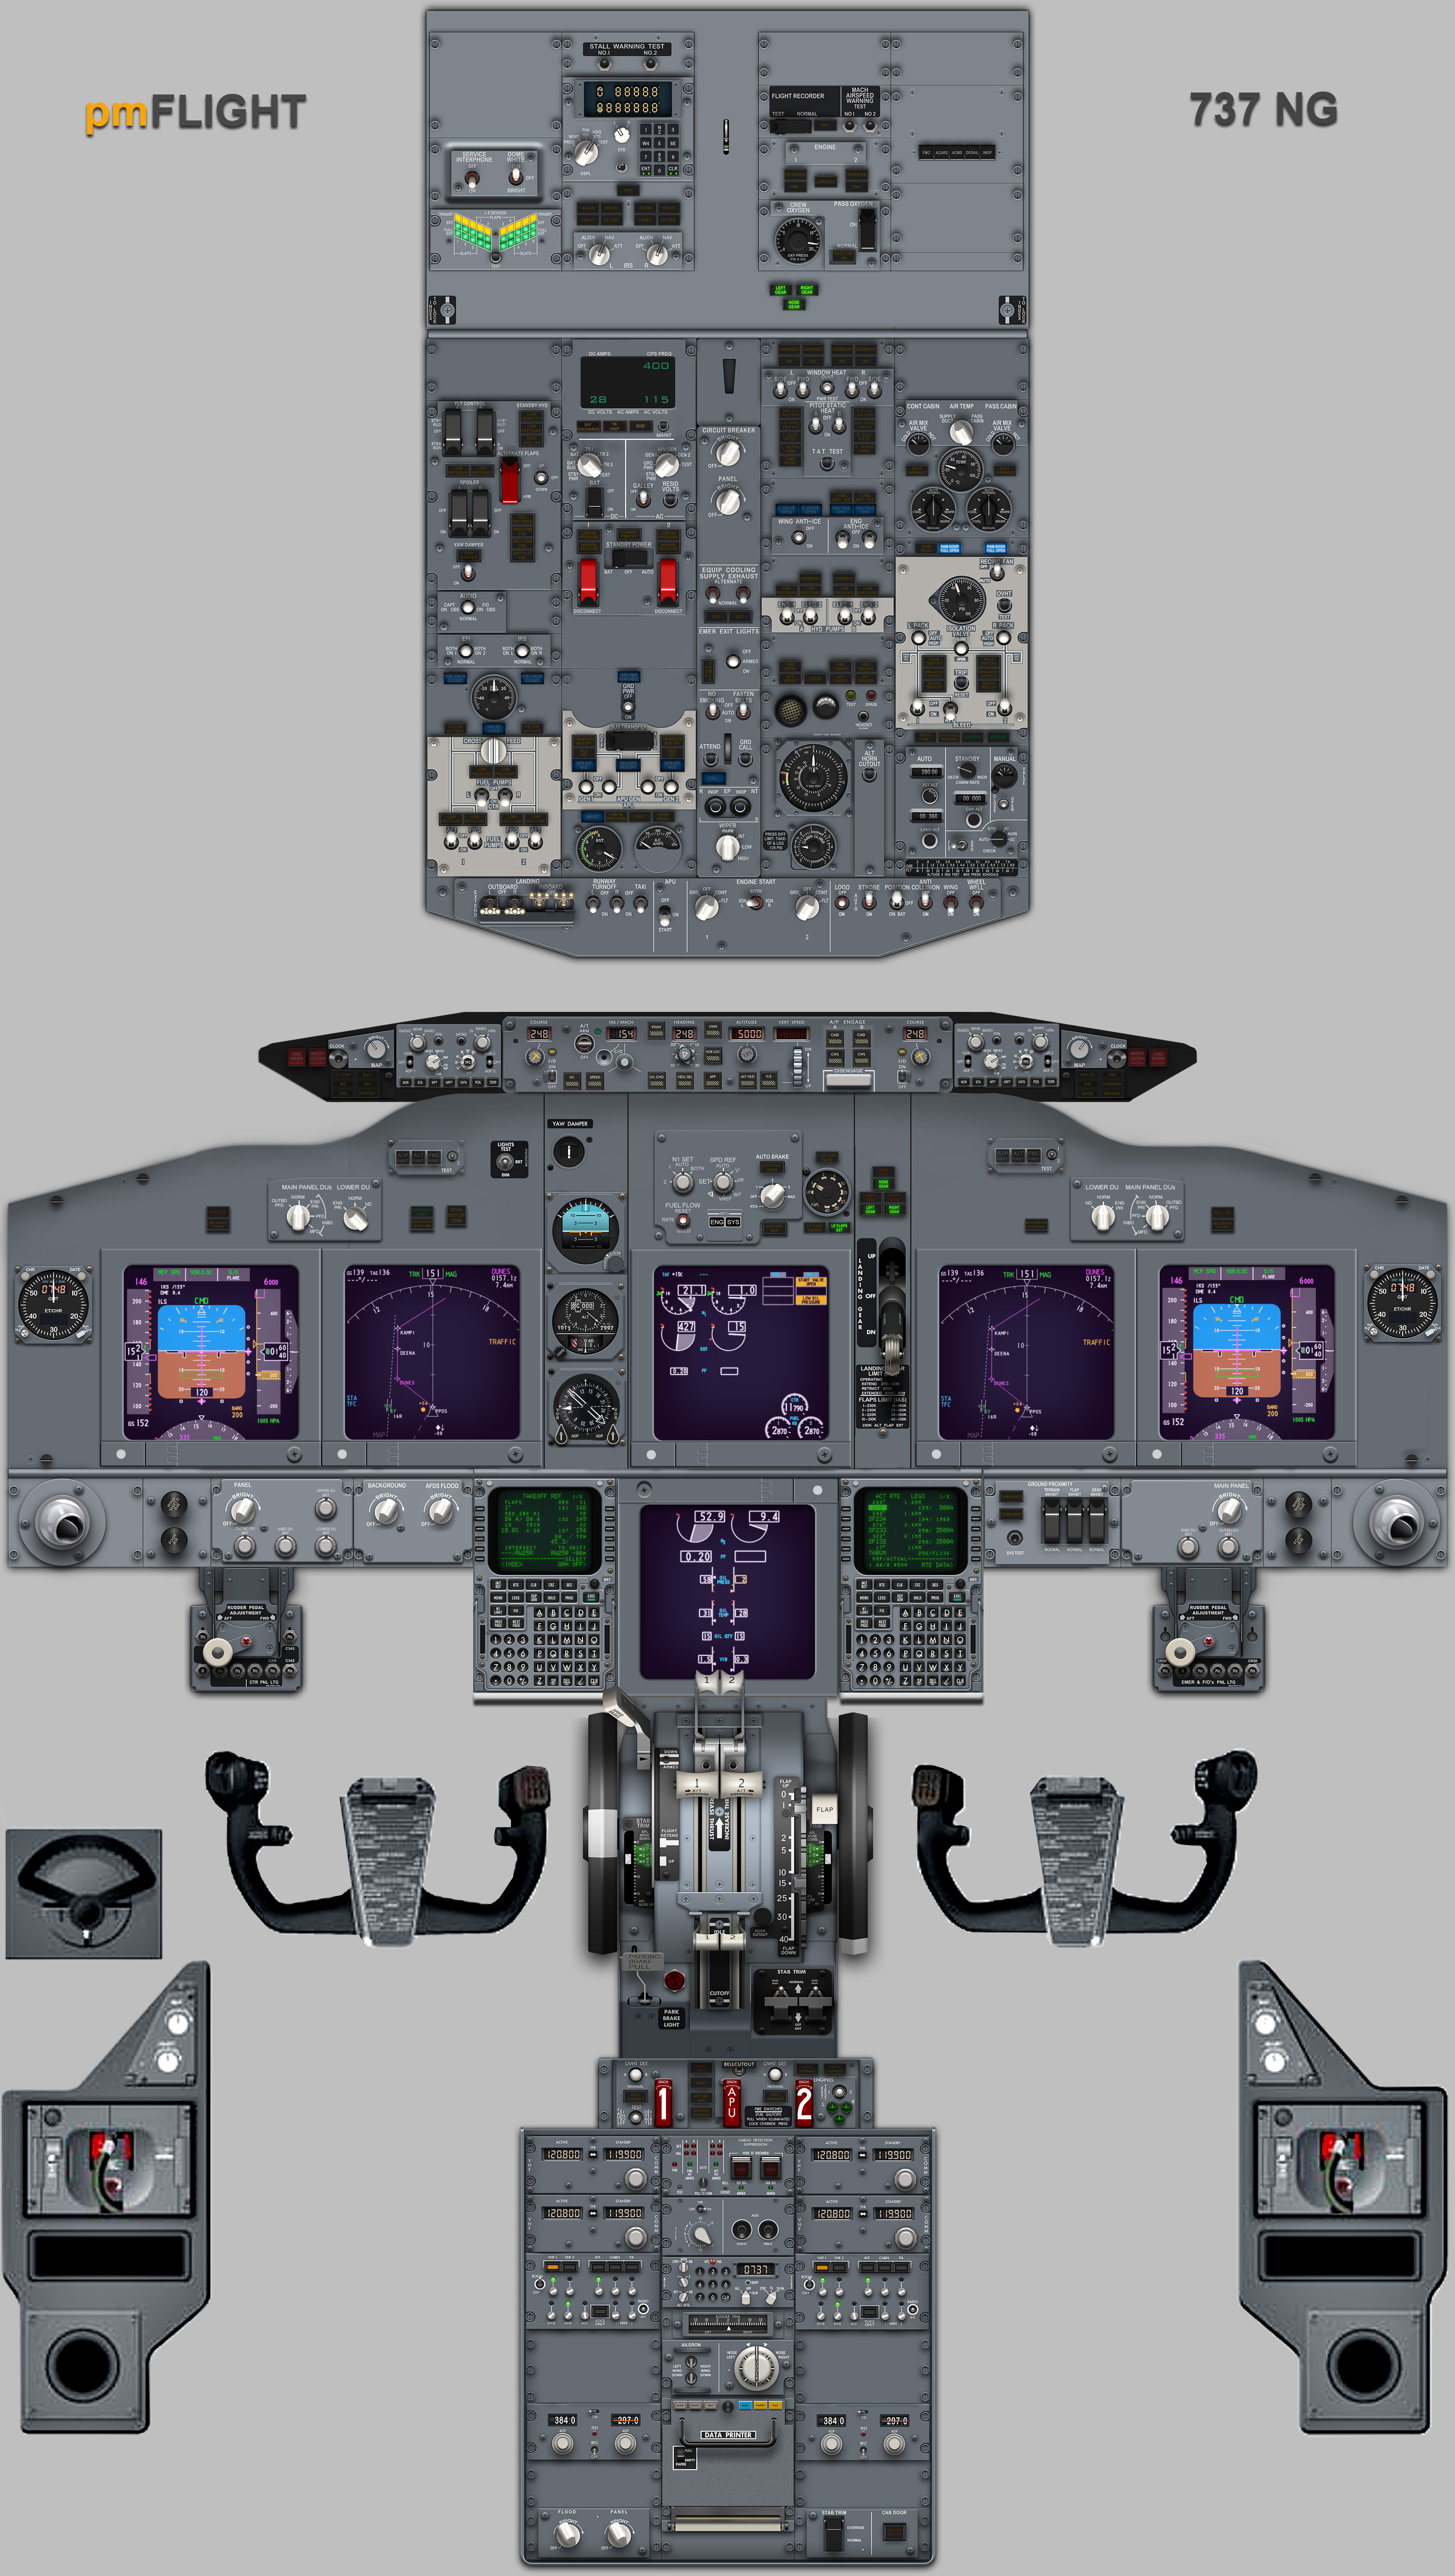
\includegraphics[width=0.6\textwidth]{01.tablero.instrumentos/U01.imagenes/1.2.distribucion.normalizada.instrumental.en.tablero/01-free-737-poster-HI.jpg}

  \caption{Cabina del Boeing 737 NG. Gentileza \protect\href{https://pmflight.co.uk}{pmFlight}}
  \label{fig:01.cabina.boeing.737NG}
\end{figure}

\begin{figure}[!htb]
  \centering
    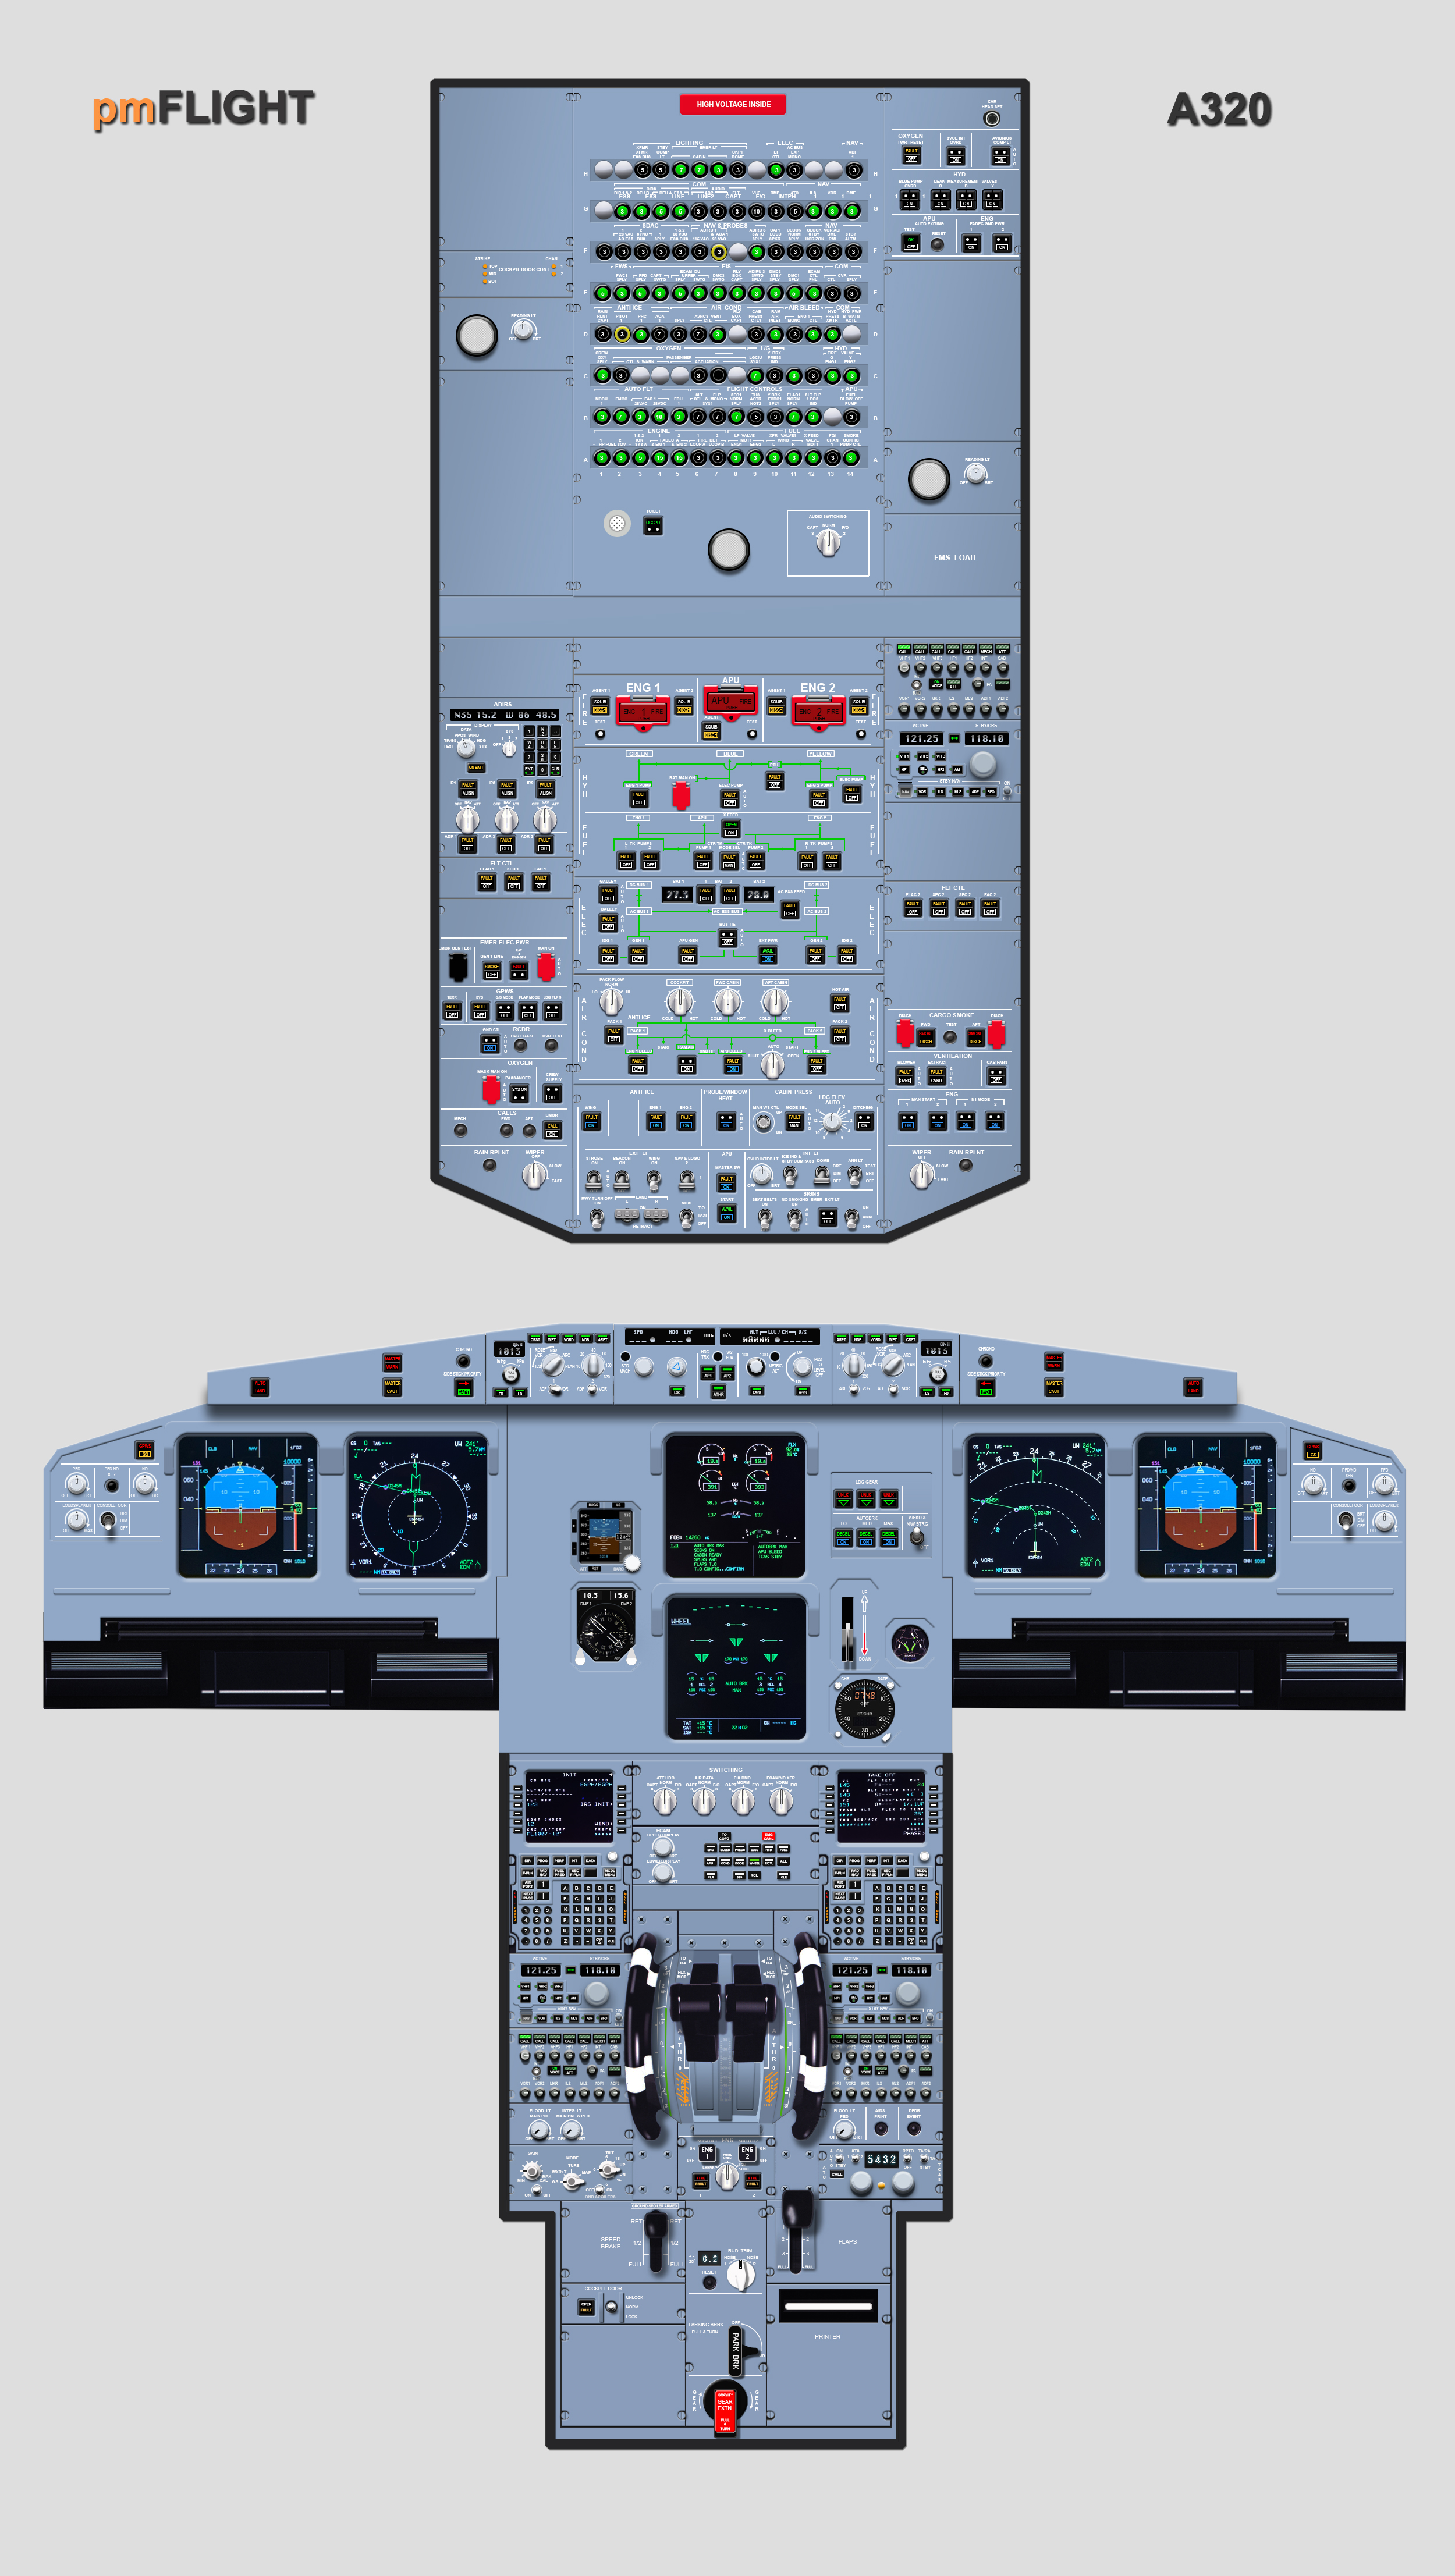
\includegraphics[width=0.6\textwidth]{01.tablero.instrumentos/U01.imagenes/1.2.distribucion.normalizada.instrumental.en.tablero/01-free-airbus-a320-poster-HI.jpg}

  \caption{Cabina del Airbus A320. Gentileza \protect\href{https://pmflight.co.uk}{pmFlight}}
  \label{fig:01.cabina.boeing.A320}
\end{figure}




\section{Presentaci\'on en Pantalla Electr\'onica}
\label{sec:presentacion.en.pantalla.electronica}

{Un poco de historia...}


        \begin{description}
        \item[1970] NASA investigaci\'on en como mostrar instrumentos
          de vuelo
        \item[1982]Boeing 767 con pantallas electr\'onicas de datos tipo \ac{CRT}
        \item[1990]Fines de la d\'ecada, pantallas \ac{LCD} reemplazan
          pantallas \ac{CRT}, ver Figura \ref{fig:01.CRT}.
        \item[Actualidad] La mayor\'ia de las aeronaves equipadas con
          pantallas \ac{LCD}, ver Figura \ref{fig:01.LCD}.
        \item[Futuro] Uso de pantallas tipo \ac{OLED} y empleo de pantallas t\'actiles, ver Figura \ref{fig:01.04.cabina.actual.vs.cabina.futura} y Figura \ref{fig:01.OLED}.
        \end{description}

        \begin{figure}
          \centering
          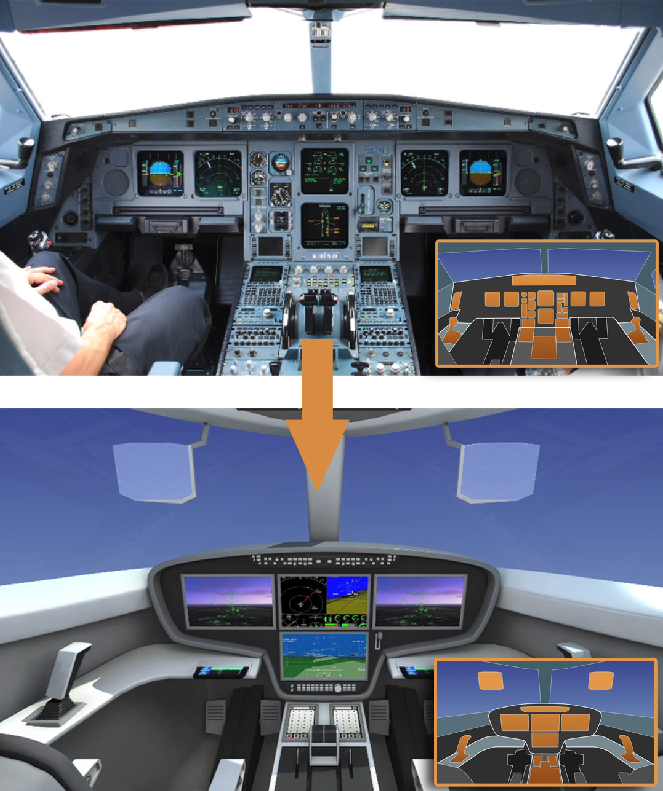
\includegraphics[width=0.8\linewidth]{01.tablero.instrumentos/imagenes/1.4.pantalla.electronica/01_04_cabina_actual_vs_cabina_futura.png}
          \caption{Cabina actual y cabina futura con pantallas t\'actiles \protect\cite{Bonelli2011FlyingWC}}
          \label{fig:01.04.cabina.actual.vs.cabina.futura}
        \end{figure}


\begin{tcolorbox}
La empresa Thales ha presentado FlytX, la nueva generaci\'on de cabina de vuelo con pantallas t\'actiles para aeronaves y helic\'opteros, mayor informaci\'on puede encontrarse 
\href{https://www.thalesgroup.com/en/markets/aerospace/flight-deck-avionics-equipment-functions/flytx-tactile-large-display-flight-deck}{aqu\'i} 
y un video de la misma 
\href{https://www.youtube.com/watch?v=PcrEUL8ATgE}{aqu\'i}.
\end{tcolorbox}

\begin{figure}[!htb]
  \centering
  \subfigure[CRT]{\includegraphics[width=0.75\linewidth]{01.tablero.instrumentos/imagenes/1.4.pantalla.electronica/CRT.gif} \label{fig:01.CRT}}

  \subfigure[LCD]{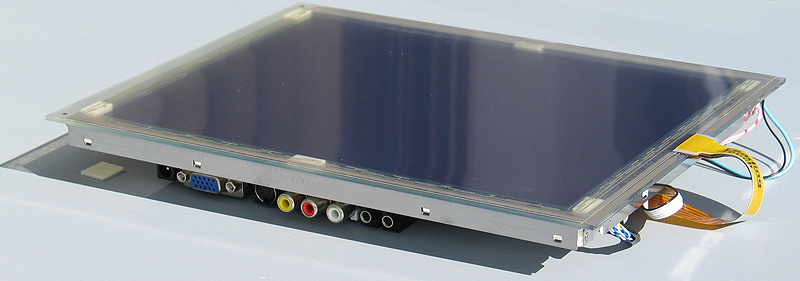
\includegraphics[width=0.45\linewidth]{01.tablero.instrumentos/imagenes/1.4.pantalla.electronica/LCD.jpg} \label{fig:01.LCD}}
  \subfigure[OLED]{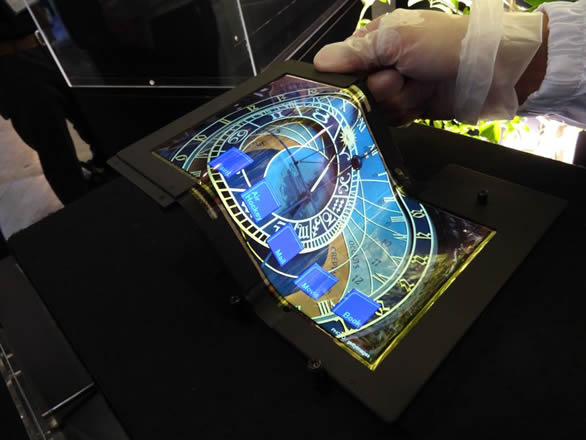
\includegraphics[width=0.45\linewidth]{01.tablero.instrumentos/imagenes/1.4.pantalla.electronica/foldable-oled-display.jpg} \label{fig:01.OLED}}
  
  \caption{Diferentes tipos de tecnolog\'ia de pantallas}
\label{fig:01.diferentes.tecnologias.pantallas}
\end{figure}



  \subsection{ \ac{EIS}}
  \label{sec:01.EIS}

  El sistema comprende el \ac{EFIS} y al \ac{ECAM}  tal como se muestra en la Figura \ref{fig:01.eis}. 

  \begin{figure}[!htb]
    \centering
    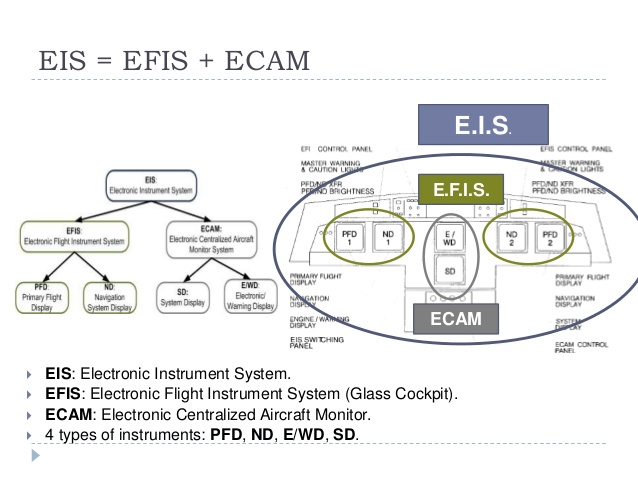
\includegraphics[width=\textwidth]{01.tablero.instrumentos/U01.imagenes/1.4.pantalla.electronica/01_eis.jpg}
    \caption{EIS}
    \label{fig:01.eis}
  \end{figure}

%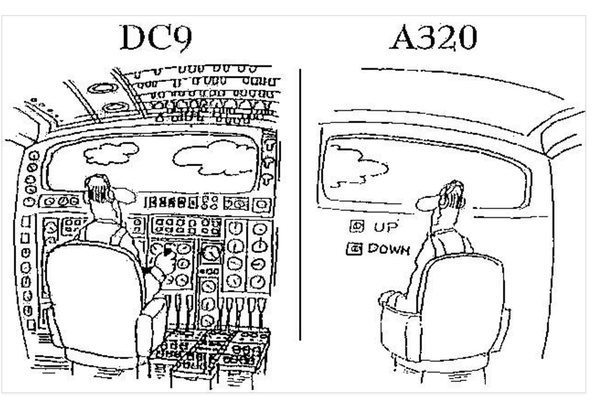
\includegraphics[width=0.5\textwidth]{01.tablero.instrumentos/imagenes/1.4.pantalla.electronica/efis_humor.png}


% Ejemplos:

% 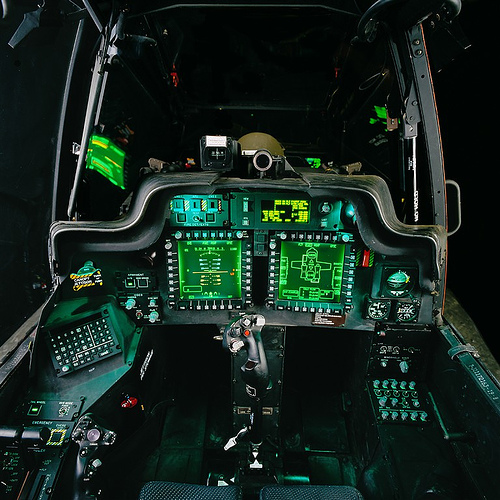
\includegraphics[width=0.34\textwidth]{01.tablero.instrumentos/imagenes/1.4.pantalla.electronica/apache.jpg}
% \hspace{3mm}
% 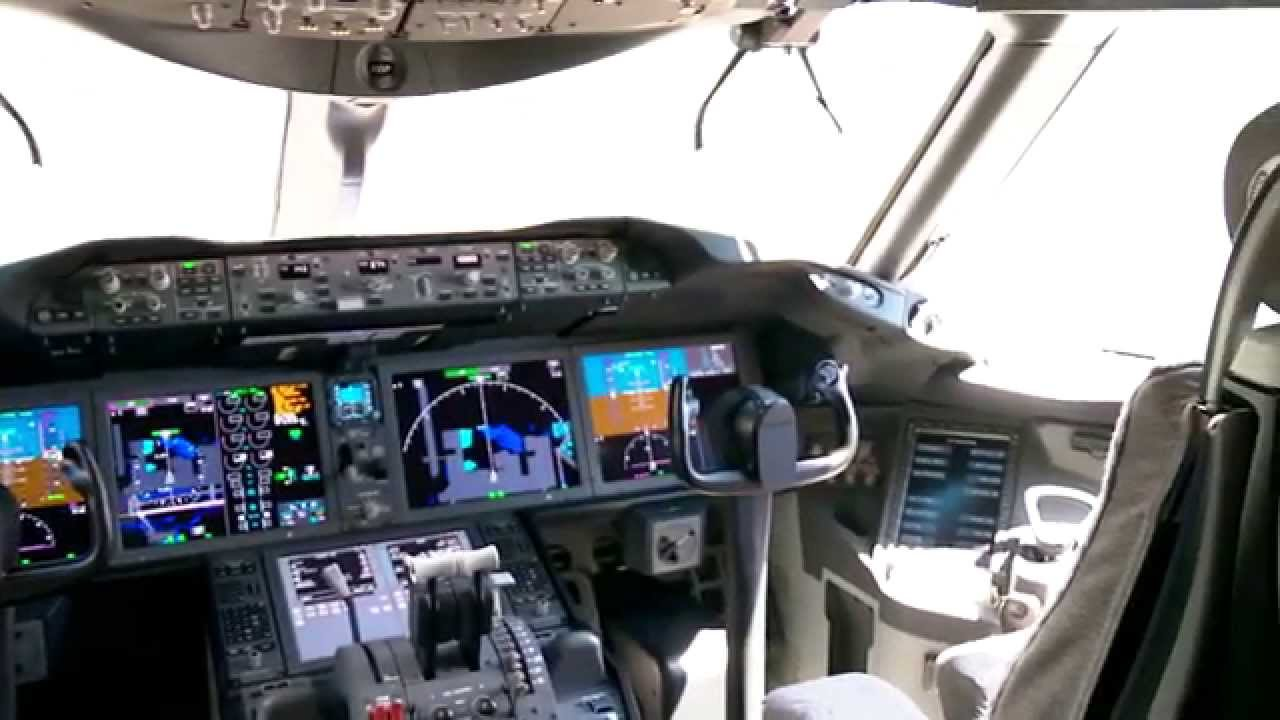
\includegraphics[width=0.55\textwidth]{01.tablero.instrumentos/imagenes/1.4.pantalla.electronica/dreamliner.jpg}

% Helic\'optero Apache \hspace{25mm} Boeing 787 Dreamliner


Una instalaci\'on \ac{EIS} sigue la secuencia siguiente:

\vspace{3mm}


 Pantallas \qquad $\Longrightarrow$ \qquad
 Controles  \qquad $\Longrightarrow$ \qquad
 Procesadores de datos 

 \begin{tcolorbox}
   El sistema EIS est\'a brevemente explicado  
   \href{https://www.youtube.com/watch?v=AS91uq1tkjQ}{aqu\'i} y \href{https://www.youtube.com/watch?v=2aix7kIL29o}{en este video}
 \end{tcolorbox}


\subsection{EFIS}
\label{sec:01.efis}


Como ejemplo de \ac{EFIS} se tiene el producto 
\href{http://www.ifd-net.com/}{IFD-NET EFIS de M.A.V.AVIONIC DIVISION}  que proveen un manual de especificaciones del producto y de instalaci\'on.


Video interesante con detalle de uso de la cabina de un Airbus 350 
\href{https://www.youtube.com/watch?v=jk-WClye4bw}{Airbus A350 Lufthansa ULTIMATE COCKPIT MOVIE + Business Class Tokyo [AirClips full flight series]}


\subsubsection{\ac{PFD}}
\label{sec:01.pfd}

	El PFD reemplaza a los seis (6) instrumentos tradicionales.
	Muestra la informaci\'on cr\'itica de vuelo 
	incluyendo velocidad, altitud,direcci\'on (heading)
	actitud y velocidad vertical.

	Est\'a dise\~nado para mejorar las alertas al piloto
	al integrar informaci\'on en una sola pantalla.
	Reduce el tiempo para monitorear otros instrumentos.

	Alerta a los pilotos de condiciones potencialmente peligrosas
        cambiando el color o la forma en el display o mediante alertas
        de sonido (baja velocidad, alta tasa de descenso). 

        \begin{figure}[!htb]
          \centering
          \subfigure[PFD]{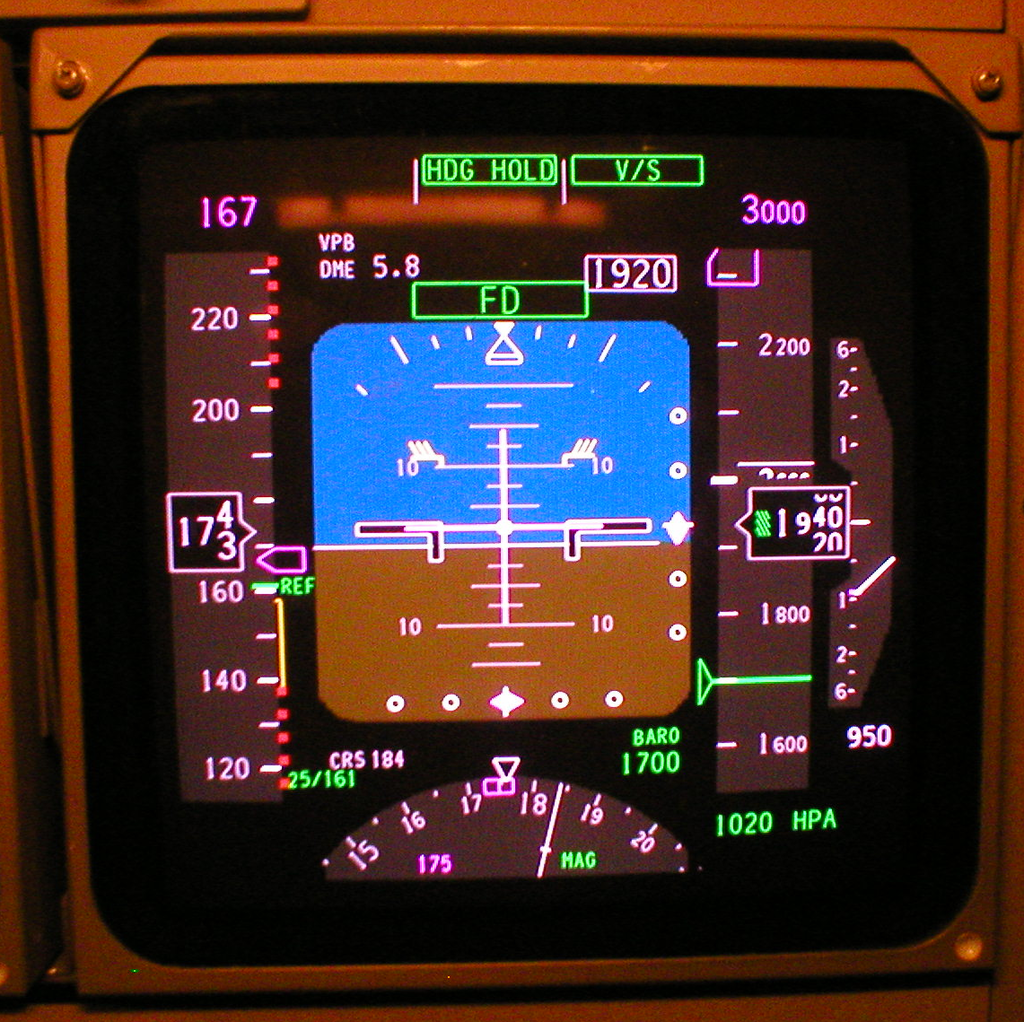
\includegraphics[width=0.45\textwidth]{01.tablero.instrumentos/U01.imagenes/1.4.pantalla.electronica/Primary_Flight_Display,_Boeing_747-400.png}
          }
          \subfigure[PFD]{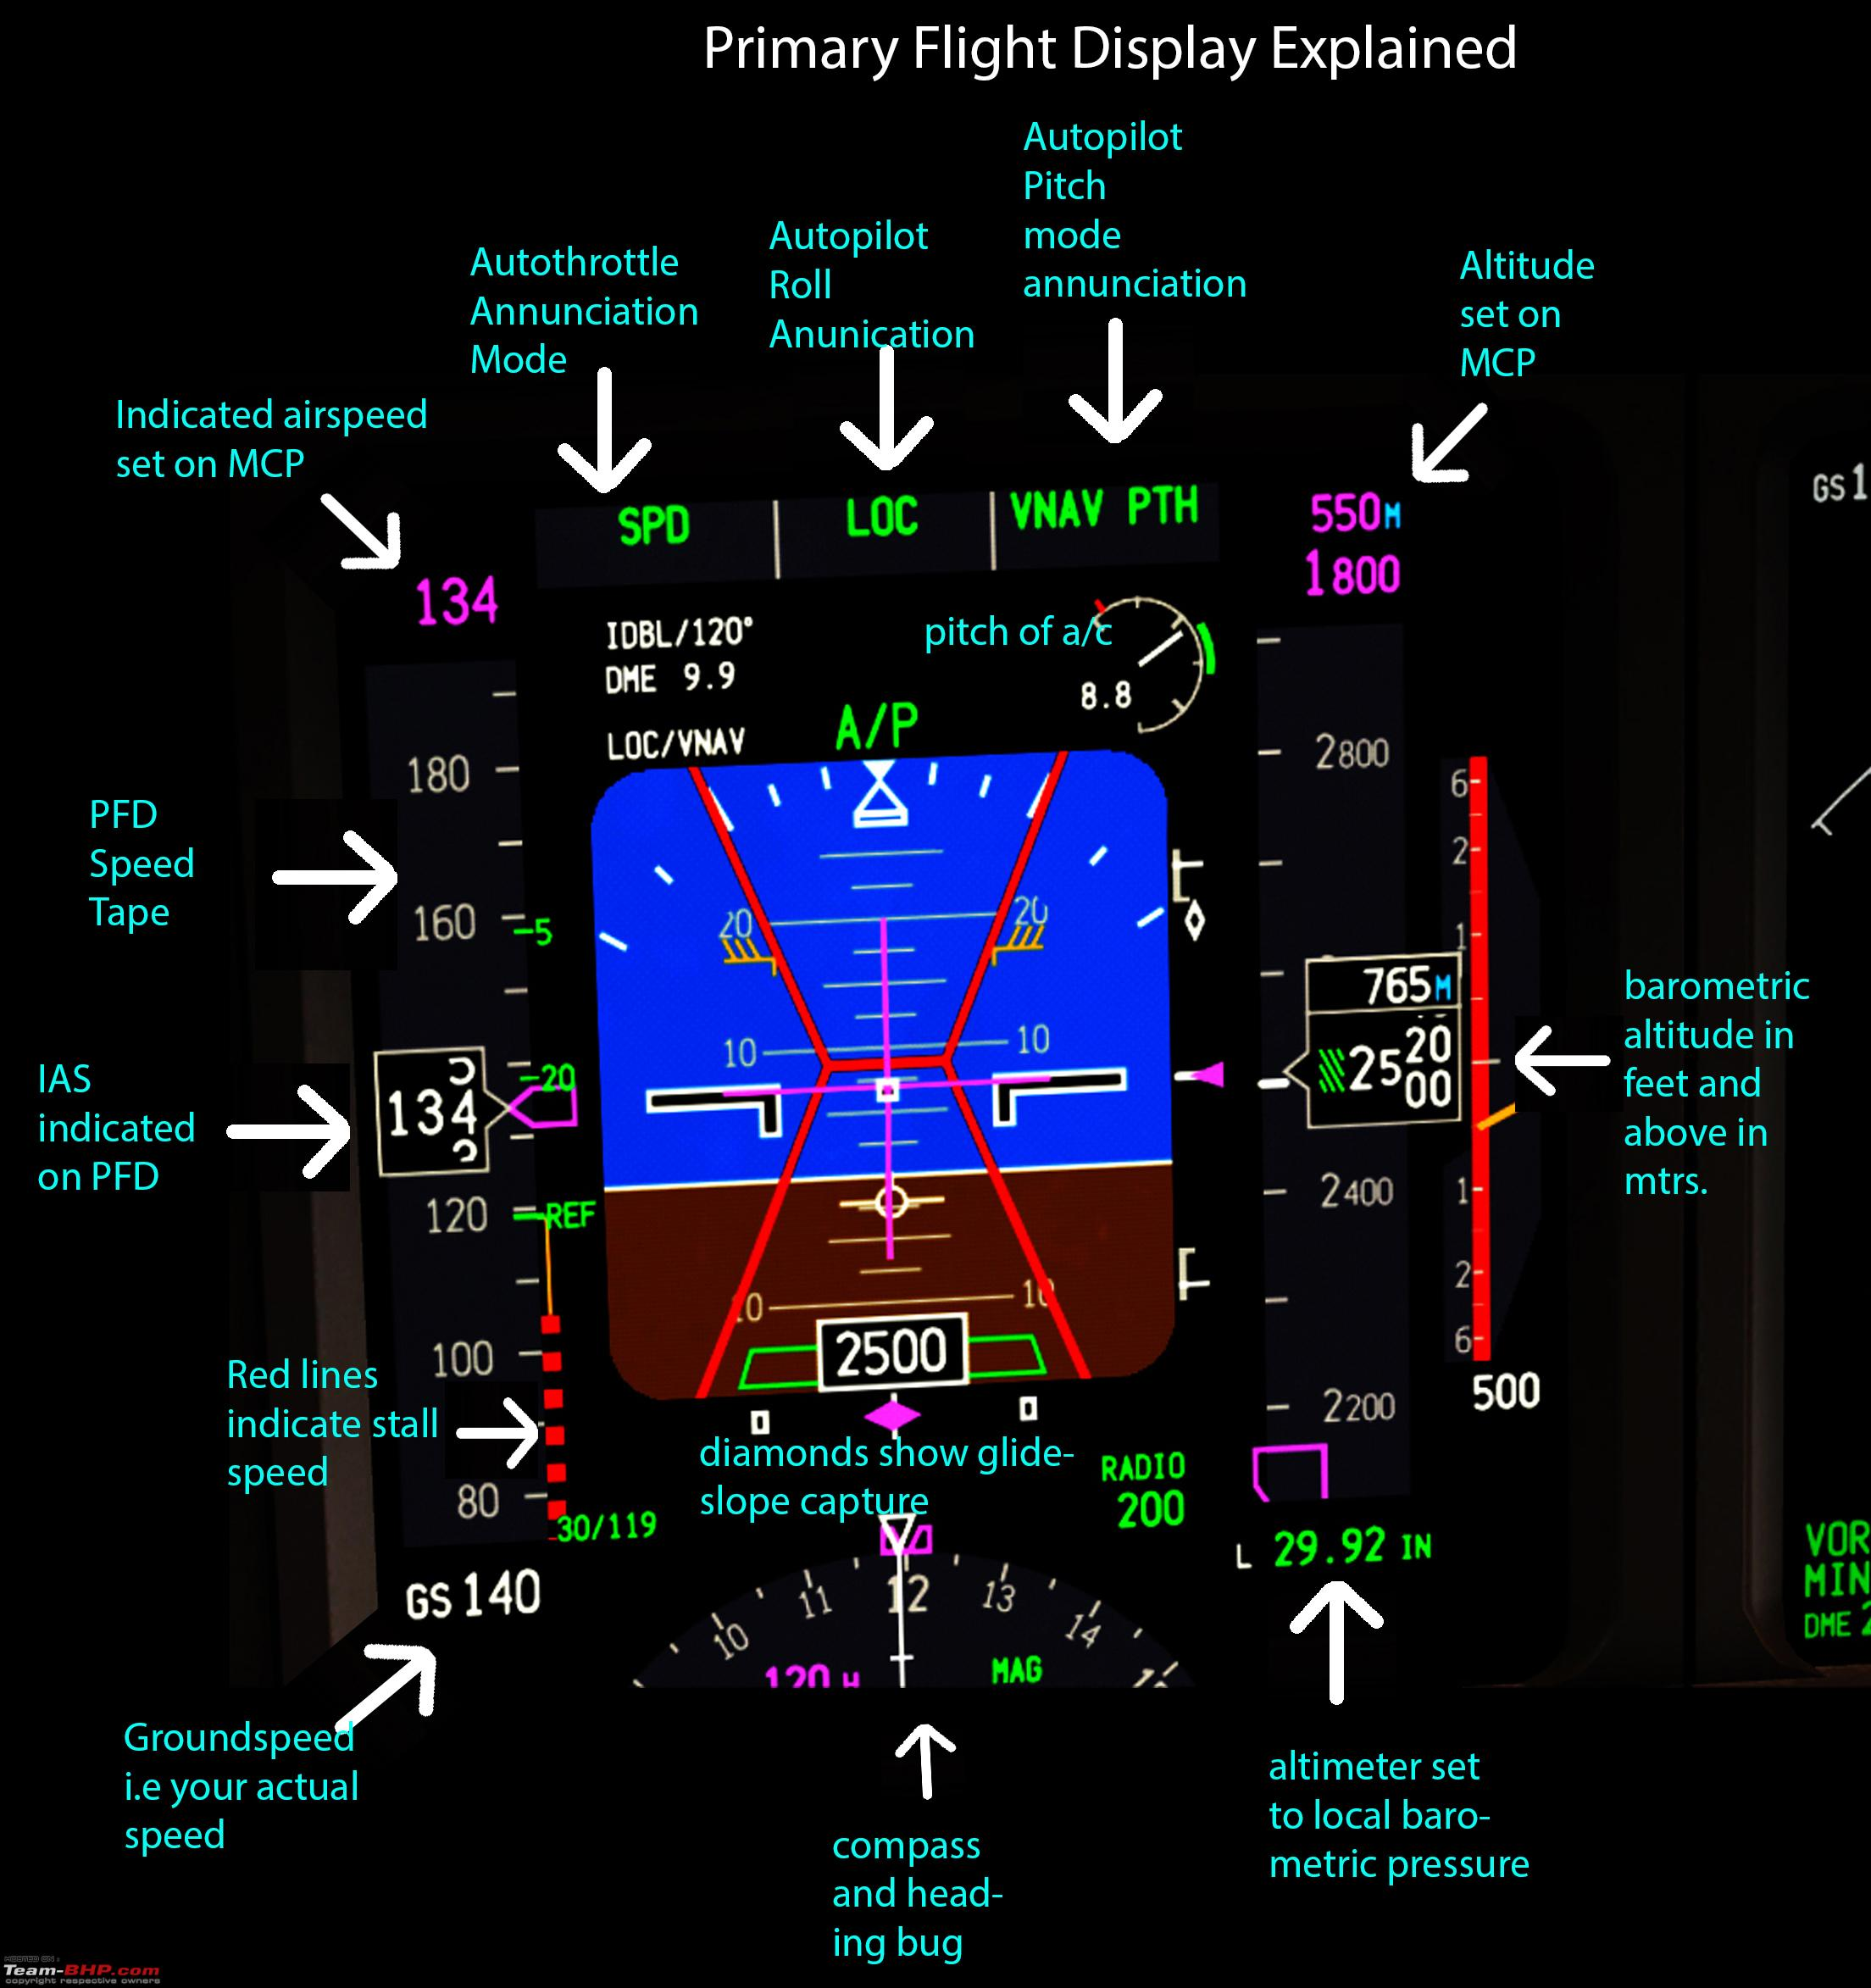
\includegraphics[width=0.45\textwidth]{01.tablero.instrumentos/U01.imagenes/1.4.pantalla.electronica/01_pfd_explanation.jpg}
          }
          
          \caption{PFD}
      \label{fig:01.pfd}
    \end{figure}


\subsubsection{\ac{ND}}
\label{sec:01.nd}

Tambi\'en es conocida como \ac{MFD}

    Provee informaci\'on para navegaci\'on (VOR, DME, ILS), iInformaci\'on clim\'atica de m\'ultiples sistemas (radar a bordo, sensores de detecci\'on de rel\'ampagos).

    Idem al PFD el MFD puede cambiar color, forma y dar alertas  sonoras.

    \begin{figure}[!htb]\centering
      
      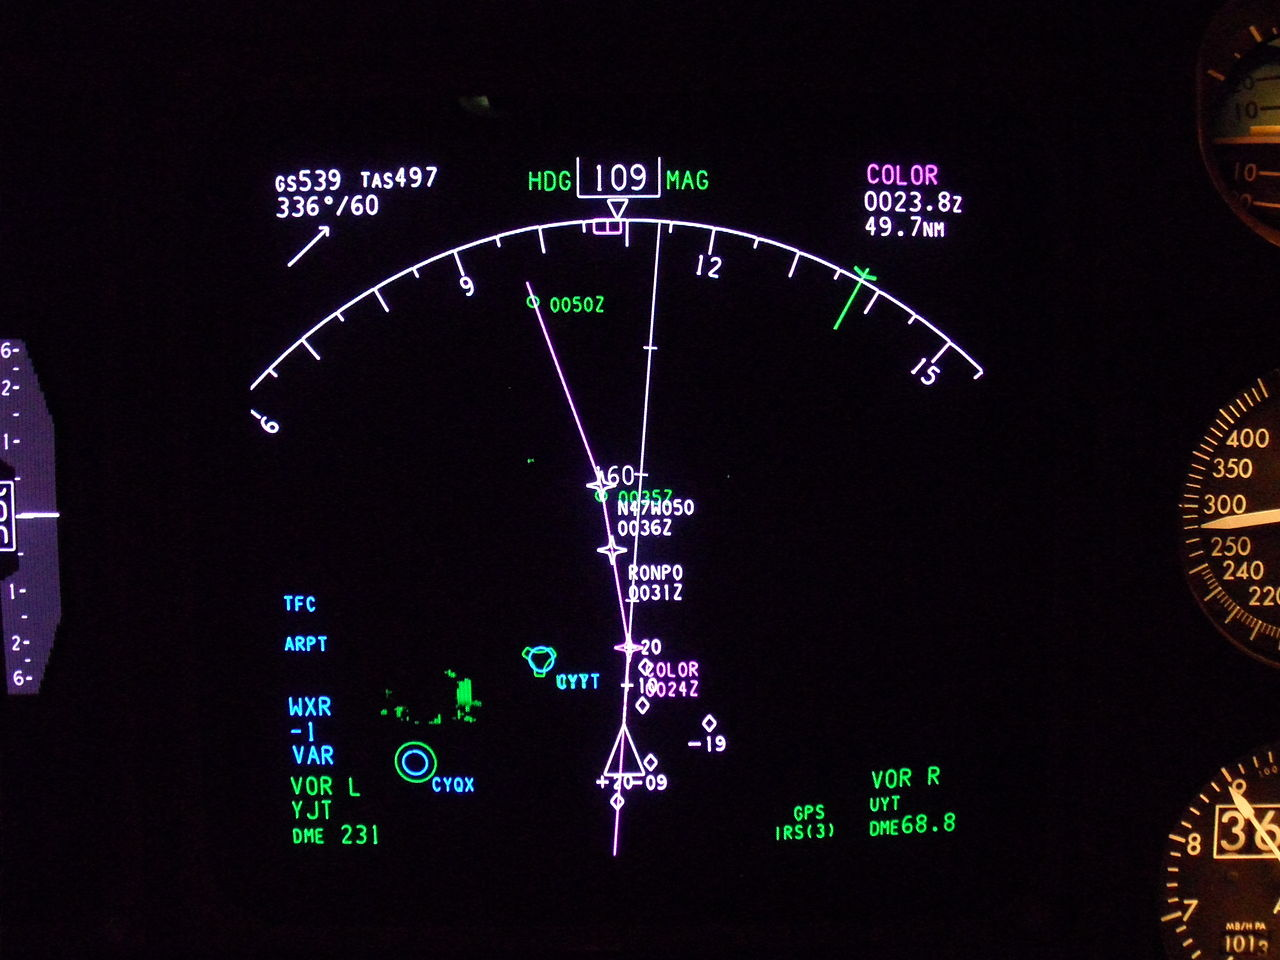
\includegraphics[width=0.45\textwidth]{01.tablero.instrumentos/U01.imagenes/1.4.pantalla.electronica/Navigation_Display_(ND)_on_Boeing_747-400.jpg}
      
      \caption{MFD o ND}
  \label{fig:01.MFD}
\end{figure}

\subsubsection{\ac{FMS}}
\label{sec:01.FMS}

   Instrumentos para mantener el plan de vuelo (flight plan) permite
    a los pilotos modificarlo en vuelo

    Dada la posici\'on y el plan de vuelo, el  \ac{FMS} se encarga de guiar
    el avi\'on a lo largo del mismo, gestiona los diversos factores
    que afectan al vuelo del avi\'on, tanto la ruta que tiene que
    seguir, como los niveles \'optimos a los cuales volar para reducir
    el consumo y hacer un vuelo m\'as eficiente.


    Usualmente se presenta como una pantalla peque\~na y un teclado

    El \ac{FMS} se compone principalmente del \ac{CDU} y 
    el \ac{FMC}
 
El piloto introduce los datos al \ac{FMC} a trav\'es de la \ac{CDU} que no es m\'as que un teclado 
y una pantalla que sirve para la comunicaci\'on entre el piloto y el \ac{FMC}. 
A trav\'es de la \ac{CDU} el piloto programa la ruta del vuelo, las \ac{SID}  
y las \ac{STAR}, as\'i como los puntos en las rutas donde el avi\'on debe ascender 
a niveles \'optimos seg\'un disminuye el peso del avi\'on.

\begin{figure}[!h]
  \centering
  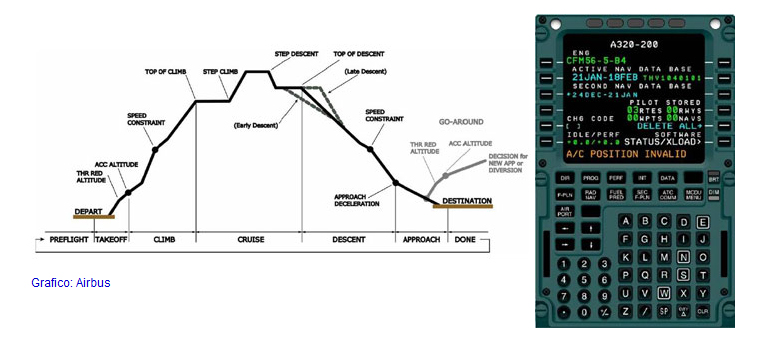
\includegraphics[width=0.9\textwidth]{01.tablero.instrumentos/imagenes/1.4.pantalla.electronica/fms_plan_vuelo.jpg}
   \caption{FMC}
\label{fig:01.FMC}
\end{figure}

El \ac{FMC} adem\'as adquiere datos de muchos de los sistemas del avi\'on. Para empezar recibe informaci\'on de los inerciales, y de los \ac{GPS} para triangular la posici\'on del avi\'on y tener una posici\'on a\'un m\'as exacta de donde se encuentra el avi\'on.

El \ac{FMS} tiene principalmente dos bases de datos. Una base de datos de navegaci\'on, donde est\'an almacenadas las rutas, aerov\'ias, \ac{SID}, \ac{STARS}, as\'i como las frecuencias de las radio ayudas a la navegaci\'on que va a sintonizar autom\'aticamente a lo largo de la ruta. Esta base de datos se renueva cada 28 d\'ias para poder estar actualizada cuando se producen cambios en los espacios a\'ereos o se modifican procedimientos de aproximaci\'on. 
El \ac{FMC} es capaz de guardar dos (2)  bases de datos de navegaci\'on.

La otra base de datos es de performance del avi\'on. Esta base de datos contiene informaci\'on de los niveles \'optimos de vuelo dependiendo del peso del avi\'on. Los consumos que tiene el avi\'on para cada peso y nivel de vuelo. Las predicciones de ascenso y descenso del avi\'on.

Como el avi\'on va envejeciendo a lo largo de su vida y disminuyendo sus performance, el \ac{FMS} admite un valor de degradaci\'on de las performance que se introduce en la p\'agina principal del \ac{CDU} para que de unas previsiones de combustibles m\'as reales seg\'un el avi\'on se va haciendo ``mayor''

Con el tiempo el \ac{FMS} ha ido mejorando y abarcando nuevas posibilidades. As\'i Airbus cambia el nombre 
al \ac{CDU} y le ha pasado a llamar \ac{MCDU}. Ahora no solamente se puede acceder 
al \ac{FMC} a trav\'es del teclado de la \ac{CDU} si no a una infinidad de nuevos servicios.

Mediante el \ac{MCDU} se accede al \ac{ATSU}, \ac{AIDS}, \ac{CFDS} y al \ac{FMS} 
comentado hasta ahora y llamado por Airbus \ac{FMGS}.

\begin{itemize}
\item El \ac{ATSU} es el acceso al Acars o sistema de comunicaciones
  tanto con la compa\~n\'ia como con el control a\'ereo. A trav\'es de
  esta opci\'on se recibe desde la hoja de carga, cualquier mensaje
  escrito que envie la compa\~n\'ia, hasta la autorizaci\'on para
  ingresar a otro pa\'is.

\item   El \ac{CFDS} es usado principalmente por el personal de
  mantenimiento.  En el est\'an los reportes de mantenimiento del
  vuelo, y las aver\'ias que haya tenido el avi\'on, por muy
  peque\~nas o temporales que hayan sido (aunque haya sido un fallo
  temporal de cualquier fusible por menos de 1 sg se queda
  registrado).

\item   El \ac{AIDS} es otra herramienta que maneja mantenimiento, sirve
  para interrogar y realizar TEST a cualquier sistema del avi\'on para
  conocer en qu\'e estado de operatividad se encuentra.
\end{itemize}


\begin{figure}[!h]
  \centering
  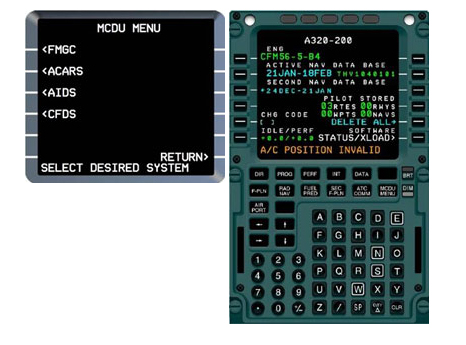
\includegraphics[width=0.9\textwidth]{01.tablero.instrumentos/imagenes/1.4.pantalla.electronica/mcdu.jpg}
  \caption{MCDU}
\label{fig:01.MCDU}
\end{figure}

\subsection{EICAS y ECAM}
\label{sec:01.eicas+ecam}

El \ac{EICAS} ha sido desarrollado por Boeing para proporcionar toda la instrumentación del motor y anuncios de tripulación en un formato integrado, 
por otra parte, el sistema utilizado en los aviones Airbus es el \ac{ECAM}. 
Los dos sistemas operan con filosof\'ias diferentes: ambos sistemas producen mensajes de advertencia, precaución y aviso que deben ser evaluados por la tripulación; en ciertos casos, el sistema indica los procedimientos necesarios para abordar el problema. 
Cada sistema utiliza  pantallas LCD o  CRT,  sus funciones básicas son monitorear los sistemas de la aeronave y mostrar información relevante a los pilotos. En la Figura \ref{fig:eicas+ecam} puede apreciarse la presentaci\'on de dichos sistemas.


\begin{figure}[!h]
  \centering
  \subfigure[EICAS en cabina de Boeing 747-400 \protect\cite{747-400-cabina}]{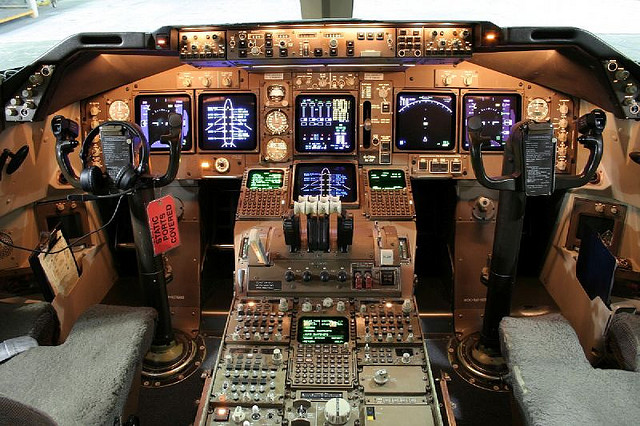
\includegraphics[width=0.45\textwidth]{01.tablero.instrumentos/imagenes/1.4.pantalla.electronica/01_Boeing_747-400_cockpit.jpg}}
  \subfigure[ECAM \protect\cite{NASA_Mumaw}]{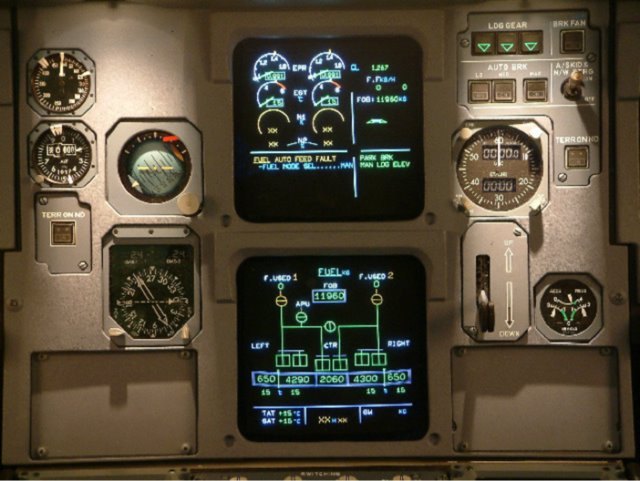
\includegraphics[width=0.45\textwidth]{01.tablero.instrumentos/imagenes/1.4.pantalla.electronica/Airbus-ECAM-displays_W640.jpg}}
  \caption{EICAS y ECAM}
  \label{fig:eicas+ecam}
\end{figure}


EICAS est\'a dividido en  dos pantallas: Upper EICAS ( superior) y Lower EICAS ( inferior),  
en la Tabla \ref{tab:01.eicas.presentacion.en.pantallas} se detalla la informaci\'on presentada en cada pantalla.% Conocido así por pilotos de un 747.
Este sistema provee la instrumentación de diversos parámetros del motor, por ejemplo RPM, valores de temperatura, caudal y cantidad de combustible, presión de aceite, etc. 
Los otros sistemas de la aeronave controlados por EICAS son; hidráulica, neumática, eléctrica, de deshielo, control de los sistemas de superficie. 
Mediante este sistema se sustituye a todos los medidores analógicos con software impulsado por pantallas electrónicas.

\begin{table}[!h]\centering
\caption{EICAS presentaci\'on en sus pantallas}
\label{tab:01.eicas.presentacion.en.pantallas}
  
\begin{tabular}{m{0.3\textwidth}m{0.65\textwidth}} \hline \rowcolor{yellow!30}
{\bf Pantalla} & {\bf Funciones } \\ \hline
\parbox{\linewidth}{  \textbf{Pantalla Superior} \\
(Upper EICAS)
}
& Muestra datos basicos de motor, indicador del modo de potencia, 
lista de mensajes de alerta, 
conjunto de arranque en vuelo, 
tren de aterrizaje, 
flaps,
combustible,
presi\'on en los conductos de aire,
altura de la cabina. \\ \rowcolor{cyan!30}

\parbox{\linewidth}{  \textbf{Pantalla Inferior} \\ Lower EICAS}
& 
La característica principal de esta
pantalla es que tiene la flexibilidad
permitir seleccionar distintos grupos
de datos en dos formas básicas:
\textcolor{blue}{\it Datos en Cifras}, y
\textcolor{blue}{\it Cuadros Sin\'opticos}.
Tambi\'en muestra mensajes de estado. \\ \hline
\end{tabular}
\end{table}

%\href{https://docplayer.es/21099386-L-aeroteca-c-montseny-num-22-esquina-sant-joaquim-08012-barcelona-telefono-932-181-739-www-aeroteca-com-www-simutaca-com.html}{BAJAR INFORMACIÓN DE AQUÍ PARA COMPLETAR EL APUNTE}

Los cuadros sinopticos de sistemas son presentados en la Lower EICAS, consisten en esquemas que representan diferentes sistemas de la aeronave.  Se les conoce como ``{\it toy modeling}'' (modelos de juegete) y permiten a los pilotos comprobar con una mirada a la pantalla de que forma est\'an dispuestos los comandos de varios sistemas. 

\begin{myboxAzul}{}
  El sistema EICAS avisa al piloto de cualquier problema usando la
  sección de mensajes de ALERTA del EICAS SUPERIOR.  El color del
  mensaje varía según su importancia:

  \begin{itemize}
  \item \textcolor{red}{\bf ROJO} indica máximo nivel de peligro y se
    denomina WARNING.

  \item \textcolor{amber}{\bf AMBAR} es el siguiente nivel, de
    precaución, y se denomina CAUTION

  \item El ultimo nivel corresponde a simples AVISOS y puede ser de
    color \textcolor{amber}{\bf AMBAR} o {\bf BLANCO} \mbox{(STATUS)}.
  \end{itemize}
\end{myboxAzul}

Los WARNING y CAUTION no pueden cancelarse

Los mensajes pueden ir acompañados por
señales ACUSTICAS.

Los mensajes STATUS del EICAS indican problemas
que pueden afectar la capacidad de funcionamiento correcto
del avión y son distintos de los mensajes ALERT.

\begin{myboxAzul}{EICAS}
  \href{https://www.youtube.com/watch?v=wSgB9FoSR5E}{
    
\includegraphics[height=1cm]{imagenes.iconos/video.jpg}
  } Video explicando como funciona EICAS.
\end{myboxAzul}

ECAM proporciona las características principales de EICAS pero también muestra las acciones correctivas que debe tomar la tripulación así como las limitaciones del sistema después de las fallas. 

Usando una jerarquía codificada por colores, la tripulación puede asimilar la información que se presenta y tomar las medidas correctivas necesarias. 
ECAM se introdujo por primera vez en el Airbus A320. En la Figura pueden observarse varias pantallas de presentaci\'on de ECAM.

ECAM comprende una serie de sistemas integrados que muestran información a la tripulación de manera eficiente. los sensores de aeronaves se clasifican en funciones clave de supervisión; estos sensores transmiten datos a dos \ac{SDAC}. Los datos se procesan y se envían a dos  \ac{FWC} que están programadas para identificar cualquier inconsistencia en los datos y luego emitir los datos a través de tres \ac{DMC}.

Si se detecta una falla o evento del sistema, uno de los FWC genera los mensajes de advertencia y alertas auditivas apropiados. Los sistemas críticos, como el motor y la cantidad de combustible, se env\'ian directamente a las FWC para que aún puedan ser monitoreados en caso de falla de ambos SDAC. 

ECAM puede tolerar la falla de un SDAC y un FWC y seguir operando. La informaci\'on es presentada en dos pantallas, una por arriba de la otra, en la Tabla \ref{tab:01.ecam.presentacion.en.sus.pantallas} se detalla la informaci\'on presentada en cada pantalla.

\begin{table}[!h]
  \centering
\caption{ECAM presentaci\'on en sus pantallas}
\label{tab:01.ecam.presentacion.en.sus.pantallas}

  \begin{tabular}{m{0.3\textwidth}m{0.65\textwidth}} \hline \rowcolor{yellow!30}
{\bf Pantalla} & {\bf Funciones } \\ \hline
  \parbox{\linewidth}{\textbf{Pantalla Superior} \\
  \ac{EWD}} 
& Muestra los principales datos del motor y otras informaciones: por ejemplo, configuración de los flaps y slats, EOR, \ac{EGT}, N1 y N2 , FUEL FLOW, mensajes y checklist en relación a operaciones normales. \\ \rowcolor{cyan!30}
  \parbox{\linewidth}{\textbf{Pantalla Inferior} \\
  \ac{SD}}
   & Presenta avisos permanentes de información adicional,  ya sea de forma automática o manual, lo cual incluye daños del sistema y sus consecuencias.  Se muestra: Indicaciones adicionales del motor, es decir, combustible utilizado, nivel de aceite, presión y temperatura de aceite niveles de vibración del motor y aviso de obstrucción de filtros de aceite y del combustible. Ademas de página de crucero, Sistema neumático, sangrando e aire ( bleed air), Sist. eléctrico, Sist. hidráulico, presurización de cabina, Sist. de combustible, APU, aire acondicionado, puertas y sistema de oxigeno, mandos de vuelo, tren de aterrizaje. \\ \hline
\end{tabular}

\end{table}

%El sinóptico típico de un sistema eléctrico se muestra en la figura 14.9. En esta ilustración, se muestran gráficamente las fuentes de energía que suministran barras colectoras específicas, junto con información como los voltajes de la batería y la unidad rectificadora del transformador (TRU) y las corrientes de suministro. La capacidad del generador se muestra como un porcentaje del máximo, junto con el voltaje y la frecuencia de salida.

Las fallas del sistema de la aeronave se priorizan como fallas de nivel 1, 2 o 3 para la pantalla superior y / o inferior. En la Tabla \ref{tab:01.ecam.jerarquia.de.advertencias.y.precauciones} se detalla la jerarquía de advertencias y precauciones.

\begin{table}[!h]
 \centering
 \caption{ECAM jerarqu\'ia de advertencias y precauciones}
 \label{tab:01.ecam.jerarquia.de.advertencias.y.precauciones}

  \begin{tabular}{m{0.10\textwidth}m{0.3\textwidth}m{0.2\textwidth}m{0.3\textwidth}} \hline \rowcolor{cyan!20}
\centering {\bf Jerarqu\'ia} & \centering {\bf Descripci\'on} & \centering {\bf Ejemplo} & \multicolumn{1}{c}{\bf Indicaci\'on} \\ \hline 

 \cellcolor{red!80} \centering \textcolor{white}{\bf Fallas de nivel 3} 
&
\begin{spacing}{0.75}
  {\scriptsize Situaciones que requieren una acción inmediata de la tripulación e indican que la aeronave está en peligro. }
\end{spacing}
& {\scriptsize Incendio en el motor o pérdida de presión en la cabina. }

& {\scriptsize Se ilumina la luz de advertencia principal roja, un mensaje ECAM de advertencia color rojo y una advertencia sonora que puede ser un timbre repetitivo continuo, un sonido específico o una voz sintética. Al presionar el botón pulsador de advertencia principal, se silencia la advertencia sonora.} \\ \hline \cellcolor{amber}

  \centering \textbf{Fallos de nivel 2} & {\scriptsize Situaciones que requieren la atención de la tripulación, pero no una acción inmediata. No tienen un impacto inmediato o directo en la seguridad del vuelo. } 

& {\scriptsize Falla de purga de aire o falla del sistema de combustible. }

&{\scriptsize Mediante una luz de advertencia principal color ámbar, un mensaje ECAM color ámbar y un pulso de timbre s\'olo.} \\ \hline \cellcolor{amber}

   \centering \textbf{Fallos de nivel 1} & {\scriptsize Estos son fallos del sistema y/o fallos que podrían provocar una pérdida de redundancia del sistema.

 Requieren monitoreo pero no tienen un impacto inmediato en la operación segura continua de la aeronave. }

&{\scriptsize La pérdida de un sensor de temperatura del sistema de combustible. }

&{\scriptsize Solamente mediante mensajes ECAM color ámbar, sin advertencia auditiva.} \\ \hline
    
  \end{tabular}
\end{table}


\section{Buses de Datos en Avi\'onica}
\label{sec:U01.05.buses.datos.avionica}

% Versión 2021
%

% la section y label cargado en el archivo madre

% \section{Buses de Datos en Avi\'onica}
% \label{sec:U01.05.buses.datos.avionica}

    Las se\~nales que se env\'ian entre los distintos componentes del
    EIS se transmiten por una l\'inea de transmisi\'on digital
    denominada ``{\it Bus de Datos}". Las se\~nales transmitidas son
    peque\~nos pulsos de tensi\'on en c\'odigo binario (unos y
    ceros). Seg\'un el protocolo, los unos y ceros se diferencian por
    tener valores distintos de tensiones positivas o negativas,
    variaciones de tensiones ascendentes o descendentes, falta de
    tensi\'on, etc. Los pusos de tensi\'on tienen duraciones
    extremadamente breves a fin de enviar una gran cantidad de
    informaci\'on en poco tiempo.

Estos son los pilares de los modernos sistemas de avi\'onica integrados, permitiendo el intercambio
de informaci\'on entre los diferentes sistemas de la aeronave. Transmiten la informaci\'on para
los datos de ingreso en un sistema y comunican los resultados para otros usuarios.

La palabra ``\emph{bus}'' es una contracción de la palabra griega ``\emph{ómnibus}'' cuyo significado es  ``\emph{para todos}''. Por lo tanto, en el contexto de computadoras y sistemas digitales, ``\emph{bus}'' se refiere a un sistema que permite la interconexión y el intercambio de datos entre los dispositivos en un sistema complejo. Sin embargo, se debe tener en cuenta que la ``\emph{interconexión}'' implica algo más que un cableado físico puesto que, entre otras cosas, define los niveles de tensión  y las reglas (o protocolos) que rigen la transferencia de datos.

Con una cantidad tan grande de sistemas de aviónica, una aeronave moderna requiere una cantidad considerable de cableado. Además, algunos de estos tendidos en una aeronave grande pueden tener una longitud considerable.

 \begin{myboxVerde}{\bf ¿C\'omo ahorrar peso? }
Con el correr de los años y los avances realizados en aviónica y sistemas de las aeronaves, estos se incrementan en las mismas y la comunicación entre ellos se vuelve más compleja. 

Por otra parte el cableado de una aeronave equivale a una proporción significativa de su peso sin carga y, por lo tanto, minimizar la cantidad de cableado  es una consideración importante en el diseño de aeronaves modernas, tanto civiles como militares.

\begin{minipage}[c]{0.3\linewidth}
  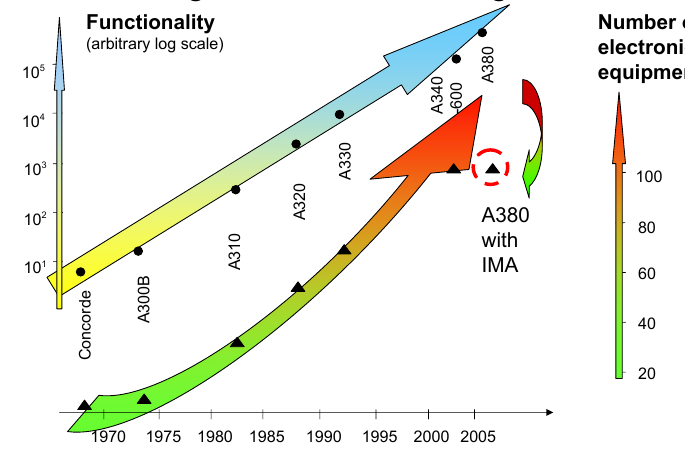
\includegraphics[width=\linewidth]{01.tablero.instrumentos/imagenes/1.5.protocolos.buses.datos/7-A380-IMA.png}
  \captionof{figure}{Aumento de sistemas de aviónica en el tiempo
   \protect\cite{a380IMA}}
\end{minipage}\hspace{1.5em}
\begin{minipage}[c]{0.3\linewidth}
  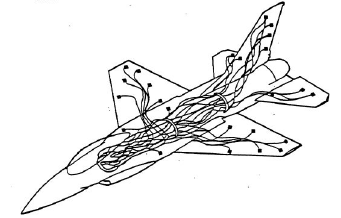
\includegraphics[width=\linewidth]{01.tablero.instrumentos/imagenes/1.5.protocolos.buses.datos/8-avion+cableado.png}
  \captionof{figure}{Conexiones punto a punto  \protect\cite{MIL-1553-tutorial} }
\end{minipage}\hspace{1.5em}
\begin{minipage}[c]{0.3\linewidth}
  \includegraphics[width=\linewidth]{01.tablero.instrumentos/imagenes/1.5.protocolos.buses.datos/9-avio+arquitectura+bus.png}
  \captionof{figure}{Conexiones con bus de datos \protect\cite{MIL-1553-tutorial} }
\end{minipage}

\end{myboxVerde}




\subsection{Conceptos generales}
\label{sec:01.05.01.01.conceptos.generales.buses}

Los sistemas de bus pueden ser unidireccionales  o bidireccionales, como se muestra en la Figura \ref{fig:01.sistemas.bus.datos}. 
También pueden ser seriales (un \ac{Bit} de datos transmitido a la vez) o paralelos (donde a menudo aparecen 8, 16 o 32 bits de datos como un grupo en varias líneas de datos transmitido al mismo tiempo). Debido a las restricciones impuestas por la longitud y el peso del conductor, todos los sistemas prácticos de bus de datos en aeronaves se basan en la transferencia de datos en serie en lugar de en paralelo.

\begin{figure}[!htb]
  \centering
  \includegraphics[width=0.4\textwidth]{01.tablero.instrumentos/U01.imagenes/U01.5.protocolos.buses.datos/01_Uni_bi_paralelo_datos.png}
  \caption{Sistemas de bus de datos. Adaptado de \protect\cite{tooley2013aircraft}}
  \label{fig:01.sistemas.bus.datos}
\end{figure}


Los sistemas de bus proporcionan un medio eficiente para intercambiar datos entre los diversos sistemas de aviónica que se encuentran en una aeronave moderna.
Las Unidades Reemplazables de Línea, en ingl\'es  \ac{LRU}, como la interfaz de datos del motor o las unidades electrónicas de flaps/slats están conectadas al bus por medio de un acoplador de bus dedicado y un módulo de interfaz en serie.

Dentro de la \ac{LRU}, la lógica digital dedicada y los sistemas de microprocesador que procesan datos localmente utilizan cada uno su propio sistema de bus local los cuales emplean, invariablemente, la transferencia de datos en paralelo que resulta ideal para mover grandes cantidades de datos muy rápidamente pero solo durante distancias cortas.

Teniendo en cuenta la temporización los buses se dividen en:
\begin{description}
\item[Síncronos] requieren de un reloj en sus líneas de control, todos los equipos trabajan con la misma velocidad.
\item[Asíncronos] requieren un ``{\it \bf handshaking}'', mediante el cual los equipos que necesitan comunicarse se ponen de acuerdo previamente.

\end{description}

Respecto a la velocidad de transmisión se tienen:

\begin{description}
\item[LS channel] o canal de baja velocidad, usualmente de cobre.
\item[HS channel] o canal de alta velocidad, de fibra óptica.
\end{description}

%PUNTO CLAVE

\begin{tcolorbox}
  Las aeronaves modernas utilizan múltiples sistemas de bus de forma
  redundante para intercambiar datos entre los diversos sistemas y
  subsistemas de aviónica. Estos sistemas de bus utilizan la
  transferencia de datos en serie porque minimiza el tamaño y el peso
  del cableado de la aeronave.
\end{tcolorbox}

\subsection{Protocolos de bus}
\label{sec:01.05.01.02.protocolos.bus}


% %La noción de un protocolo necesita una pequeña explicación. Imagine por un momento que se enfrenta con el problema de organizar una discusión entre una gran cantidad de personas sentadas alrededor de una mesa, todas las cuales están con los ojos vendados y, por lo tanto, no pueden verse. Para asegurarse de que no todos hablen a la vez, debe establecer algunas reglas básicas, incluida la forma en que los delegados indicarán que tenían algo que decir y también establecer algunas prioridades sobre quién debería hablar. en el caso de que varios delegados indiquen que desean hablar al mismo tiempo. Estas (y otras) consideraciones formarían un protocolo acordado entre los delegados para llevar a cabo la discusión. El debate debe continuar sin demasiados problemas, siempre que todos en la sala entiendan y estén dispuestos a aceptar el protocolo que ha establecido. 


% Los protocolos de comunicación permiten el intercambio eficiente de datos entre varios dispositivos conectados al mismo bus. Los protocolos consisten en un conjunto de reglas y especificaciones que rigen, entre otras cosas, el formato de datos y las conexiones físicas.


% En las computadoras y los sistemas digitales, los protocolos de comunicación se establecen para permitir el intercambio eficiente de datos entre múltiples dispositivos conectados al mismo bus.

% Una serie de estándares diferentes para protocolos se utilizan comúnmente en avi\'onica.
% Respecto a los protocolos actualmente empleados se tiene el ARINC 429, el MIL-STD 1553 y, por ultimo, el AFDX.


% \subsection{Arquitectura del bus}
% \label{sec:01.05.01.03.arquitectura.bus}

% La arquitectura de un bus de datos se refiere a la estructura general de una computadora u otro sistema digital que depende de un bus para su funcionamiento, se describe en forma de un diagrama esquemático de bloques que muestra cómo se interconectan los diversos elementos del sistema y también cómo se organiza el flujo de datos entre los elementos. 

% La arquitectura de un sistema basado en el uso de un sistema de bus serie unidireccional se muestra en la Figura 4.4a, mientras que un sistema de bus bidireccional comparable se muestra en la Figura 4.4b. Pued observarse que el sistema bidireccional simplifica la interconexión de las LRU y permite que todos los dispositivos transmitan y reciban en el mismo bus.





% \subsection{Principios del bus serie}
% \label{sec:01.05.01.04.bus.serie}

% En la Figura 4.5 se muestra un sistema simple para la transferencia de datos en serie entre dos LRU, cada uno de los cuales comprende un sistema aviónico por derecho propio. Dentro de la LRU, los datos se transfieren utilizando un bus de datos paralelo interno (8, 16, 32 o 64 bits de ancho). El enlace entre las dos LRU se realiza utilizando un cable serie simple (a menudo con solo dos, cuatro o seis conductores). La conversión de datos de paralelo a serie y de serie a paralelo se lleva a cabo mediante una interfaz de bus (a menudo se trata de una sola tarjeta o módulo dentro de la LRU). Los datos a transferir pueden ser sincrónicos (utilizando el reloj señales generadas localmente dentro de cada LRU) o pueden ser asíncronas (es decir, auto reloj).

% El sistema que se muestra en la Figura 4.5 tiene la limitación obvia de que los datos solo pueden intercambiarse entre dos dispositivos. En la práctica, necesitamos compartir los datos entre muchas LRU / unidades de aviónica. Esto se puede lograr mediante el sistema de bus ilustrado en la Figura 4.6. En este sistema, los datos se transfieren utilizando un cable de bus de par trenzado blindado, en ingl\'es ``\emph{shielded twisted pair}'',  con una serie de paneles de acoplamiento que se encuentran en los puntos apropiados de la aeronave (por ejemplo, la cubierta de vuelo, la bahía de aviónica, etc.). Cada panel de acoplamiento permite conectar varias unidades de aviónica al bus mediante un cable corto. Para optimizar la velocidad de transferencia de datos y minimizar los problemas asociados con la reflexión y la falta de coincidencia, el cable del bus debe terminarse en cada extremo utilizando un terminador de bus coincidente.

% Los acopladores de bus se producen como unidades de modo de voltaje o de modo de corriente, dependiendo de si usan dispositivos de detección de voltaje o corriente. Dentro de cada unidad LRU / aviónica, se proporciona una interfaz que realiza la conversión de datos de serie a paralelo o de paralelo a serie requerida, como se muestra en la Figura 4.7.

% Además de proporcionar una interfaz eléctrica (con el cambio apropiado de nivel de voltaje y corriente), la unidad de interfaz también convierte los formatos de datos (por ejemplo, de dobletes analógicos en serie presentes en el cable auxiliar a datos en serie codificados por Manchester requeridos por el controlador de terminal), como se muestra en la Figura 4.8. Para transmitir datos utilizando el bus de datos en serie, la información debe presentarse en un formato estándar.

% Un formato típico para datos en serie usaría una longitud de palabra de 32 bits. Esta palabra comprende varios campos discretos, que incluyen:

% \begin{itemize}
%      \item  Hasta 20 bits para datos (que pueden dividirse aún más);

%      \item Un campo de etiqueta de 8 bits que se utiliza para identificar   el tipo de datos y cualquier parámetro que pueda estar asociado a  él.

%      \item Un identificador de origen / destino (SDI);

%      \item Varios bits de estado utilizados para proporcionar informaci\'on   sobre el modo, el estado del hardware o la validez de los datos.

%      \item Un bit de paridad adicional que proporciona un medio para   validar los datos (es decir, determinar si están o no libres de   error).

% \end{itemize}

% PUNTO CLAVE

% Se requiere un medio para convertir los datos en serie en datos paralelos (y viceversa) siempre que una LRU deba conectarse a un sistema de bus de avión.





% Los buses de datos se agrupan en dos conjuntos: 

% \begin{itemize}
%     \item {\bf Simplex} o de un sentido (one way) con un \'unico transmisor y m\'ultiples receptores.
%     \item {\bf Duplex} con m\'ultiples transmisores y receptores.
% \end{itemize}




% En el panorama actual de la aviónica hemos visto pasar un número amplio de
% protocolos que han ido quedando desfasados a lo largo del tiempo. Antes de
% evaluar cada uno de ellos resulta conveniente realizar  un recorrido a la
% importancia de la aviónica en los sistemas de aviación y su evolución.

% Los sistemas han seguido creciendo
% y evolucionando haciendo que sistemas como la comunicación con los
% satélites, sistemas que controlan la electricidad o los sistemas hidráulicos sean
% controlados por electrónica.


\subsubsection{ARINC 429}
\label{sec:01.05.01.ARINC.429}

Creado por \ac{ARINC}, corporación creada en 1929 y compuesta por aerolíneas, fabricantes de aeronaves y de equipos de aviónica. \ac{ARINC} fue creada para producir especificaciones y normas para equipos de aviónica fuera del gobierno para fabricantes nacionales o internacionales.

Es un protocolo utilizado para aviones comerciales y de transporte
y nos cuenta como los equipos de aviónica se comunican unos con otros,
especifica las características eléctricas y de datos.

Se emplea en distintos aviones tanto de Airbus como de Boeing, tal
como A330 o el Boeing 747 o los helicópteros Bell. La fiabilidad de este
protocolo es a costa de un gran peso en cableado y de tasas de envío
limitadas.

El estándar ARINC 429 fue desarrollado a partir del existente estándar ARINC 419, el cual  contiene  especificaciones  de  comunicación  digital  para aviación   comercial.   En   estas   especificaciones   se tienen   cuatro   tipos diferentes  de  topologías  de  cableado,  estando  entre  ellas  una  topología  en serie  que  utiliza  un  par  trenzado  de  cable  apantallado.  Es  esta  topología  en serie la que evolucionó hacia el estándar ARINC 429. 

La primera publicación del ARINC 429 fue en Abril de 1978 y aún existe hoy día bajo  la  nomenclatura  de  ARINC  429-15.  

Este  estándar  está  dividido  en  tres partes:

\begin{description}
\item[Parte 1-15:] Descripción funcional, interfaz eléctrica,
  asignación de etiquetas y formato del paquete de datos.
\item[Parte 2-15:]   Estándares para paquetes de datos discretos. %, define los formatos de paquetes con asignación d.
\item[Parte 3-15:] Técnicas de  transferencias de datos.
\end{description}



ARINC  429  es  un  bus  de  datos   simplex que tiene las siguientes características:

\begin{itemize}
\item Está compuesto por  por dos hilos unidireccionales de datos estándar (puertos Tx y Rx), apantallados y de lazo abierto (open loop) tipo 
Mark 33 Digital Information Transfer System bus.

\item La fuente y el destino deben estar conectados mediante un par de cables trenzados y apantallados. El apantallamiento debe conectarse a masa en ambos lados de la conexión y en todos los conectores intermedios del cableado.

\item Tiene dos velocidades de funcionamiento: baja velocidad entre 12-14,5 Kbps y alta velocidad alcanzando 100 Kbps. 

\item No se pueden utilizar ambas velocidades en el mismo bus.

\item La codificación  es  RZ bipolar

\item El formato de las palabras enviadas por este protocolo es  de  palabras o paquetes de datos  de  32  bits.


\item El protocolo  establece que  debe haber   un   espacio   de   tiempo   entre   cada   palabra (o paquete de datos)   enviada  (GAP).

\item      Las características del mensaje son:
  \begin{itemize}
  \item La información fluye desde una puerta de transmisión hasta una
    o varias puertas de recepción.
  \item En ningún caso la información puede llegar hasta una puerta
    destinada a la transmisión.
  \item La transmisión entre dos LRU en ambos sentidos se
    realiza por buses independientes.
  \end{itemize}

\item El transmisor emite siempre, ya sea 32 bits de datos (palabra) o el estado nulo (NULL).

\item El bus posee un  solo  transmisor  y  hasta  20  receptores.

\item  Si  se  desea implementar  una  comunicación  bidireccional  se  necesitan  dos  canales  o  dos buses.

\end{itemize}


\begin{figure}[!h]
  \centering
%  \scalebox{0.9}{
% ARINC 429 topologias

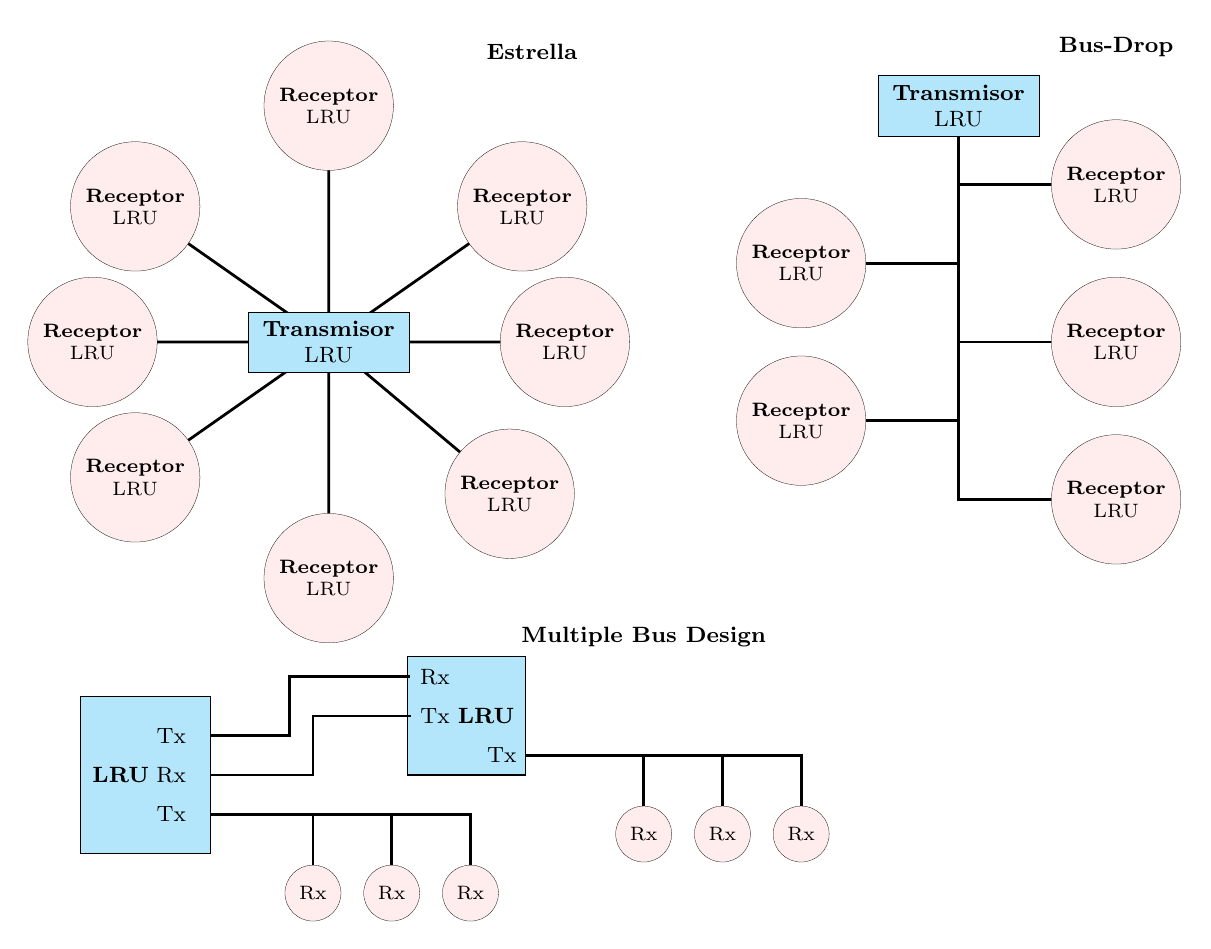
\begin{tikzpicture}[node distance=1cm, 
				font = \footnotesize , 
               Transmisor/.style ={ fill=cyan!30 , 
                          draw,
                          line width= 0.1 , 
						text width=1.8cm,
						align = center
                        } ,
               Receptor/.style ={  font = \scriptsize, 
						circle ,
                          fill=pink!30 , 
                          draw,
%						text width=1.2cm,
						align = center ,
                          line width= 0.1 , 
                        } ,
			]

% grilla
%  \draw[ green!50!black] (0,0) grid (20,10) ;

\path (3.5 , 7.5) coordinate (TxEstrella)
             (11.5 , 10.5) coordinate (TxBusDrop)
      ;

% Topologia estrella

\draw (TxEstrella) + (55:4.5) node {\bf Estrella};
\draw[line width=1]
               (TxEstrella) node[Transmisor]  {{\bf Transmisor} \\ LRU }
               -- +(0:3.0) node[Receptor]  {{\bf Receptor} \\ LRU }
(TxEstrella)  --  +(35:3.0) node[Receptor]  {{\bf Receptor} \\ LRU }
(TxEstrella)  --   +(90:3.0) node[Receptor]  {{\bf Receptor} \\ LRU }
(TxEstrella)  --   +(145:3.0) node[Receptor]  {{\bf Receptor} \\ LRU }
(TxEstrella)  --  +(180:3.0) node[Receptor]  {{\bf Receptor} \\ LRU }
(TxEstrella)  --   +(215:3.0) node[Receptor]  {{\bf Receptor} \\ LRU }
(TxEstrella)  --    +(270:3.0) node[Receptor]  {{\bf Receptor} \\ LRU }
(TxEstrella)  --    +(320:3.0) node[Receptor]  {{\bf Receptor} \\ LRU }
  ;

% Topologia estrella
\draw (TxBusDrop)  +(2,0.75)  node {\bf  Bus-Drop};
\draw[line width=1]
               (TxBusDrop) node[Transmisor]  {{\bf Transmisor} \\ LRU }
				         |- +(2,-1) node[Receptor]  {{\bf Receptor} \\ LRU }
(TxBusDrop) |- +(-2,-2) node[Receptor]  {{\bf Receptor} \\ LRU }
(TxBusDrop) |- +(2,-3) node[Receptor]  {{\bf Receptor} \\ LRU }
(TxBusDrop) |- +(-2,-4) node[Receptor]  {{\bf Receptor} \\ LRU }
(TxBusDrop) |- +(2,-5) node[Receptor]  {{\bf Receptor} \\ LRU }
;

% Topologia Multiple Bus Design

\draw [fill=cyan!30] (0.35,1) rectangle (2,3) 
	(1,2) node[text width=1cm] {\bf LRU}
		+ (0.5,0.5) node (Tx1) {Tx}
		+ (0.5,0.0) node (Rx1) {Rx}
		+ (0.5,-0.5) node (Tx11) {Tx}
;

\draw [fill=cyan!30] (4.5,2) rectangle (6,3.5) 
	(5.5,2.75) node {\bf LRU} +(2.0 , 1.0) node {\bf Multiple Bus Design}
		+ (-0.65,0.5) node (Rx2) {Rx}
		+ (-0.65,0.0) node (Tx2) {Tx}
		+ (0.2,-0.5) node (Tx22) {Tx}
;

\draw[line width=1] (Tx1) +(0.5 , 0) -- +(1.5,0) |- (Rx2) ;
\draw[line width=1] (Rx1) +(0.5 , 0) -- +(1.8,0) |- (Tx2) ;
\draw[line width=1] (Tx11) +(0.5 , 0) -- +(1.8,0) -- +(1.8 , - 1) node[Receptor] {Rx} ;
\draw[line width=1] (Tx11) +(0.5 , 0) -- +(2.8,0) -- +(2.8 , - 1) node[Receptor] {Rx} ;
\draw[line width=1] (Tx11) +(0.5 , 0) -- +(3.8,0) -- +(3.8 , - 1) node[Receptor] {Rx} ;

\draw[line width=1] (Tx22) +(0.3 , 0) -- +(1.8,0) -- +(1.8 , - 1) node[Receptor] {Rx} ;
\draw[line width=1] (Tx22) +(0.3 , 0) -- +(2.8,0) -- +(2.8 , - 1) node[Receptor] {Rx} ;
\draw[line width=1] (Tx22) +(0.3 , 0) -- +(3.8,0) -- +(3.8 , - 1) node[Receptor] {Rx} ;



\end{tikzpicture} 
%}
  \caption{Topologías ARINC 429, adaptado de \protect\cite{ARINC429Tutorial2010}}
  \label{fig:01.Topologias.ARINC429}
\end{figure}

Las  formas  de  conexión  más  utilizadas  para  conectar  las  LRU son la topología en Estrella o la Bus-Drop, Figura \ref{fig:01.Topologias.ARINC429}, donde cada LRU puede contener múltiples receptores y transmisores.

La mayor parte de la topología emplea una arquitectura punto a punto lo que proporciona alta fiabilidad en la transferencia de información.

\begin{myboxAzul}{Características del cableado}
  En este bus de
  comunicación se utiliza un par de cable trenzado y apantallado con
  una impedancia de 78$\Omega$.  El apantallamiento debe ir conectado
  a tierra al final de cada tramo y en cada unión de líneas.

La impedancia de salida del transmisor debe ser de $75 \Omega \pm 5 \Omega$
divididos equitativamente entre las líneas A y B, esta salida balanceada debe coincidir con la impedancia del cable. El receptor debe tener una impedancia efectiva de ingreso de $8\Omega$ como mínimo.

No se especifica una longitud máxima para los conductores, la mayoría de los sistemas emplean menos de 150 pies pero, si las condiciones lo permiten se puede llegar al doble de esta longitud o más.

\end{myboxAzul}
%\begin{myboxAzul}{Paquete de datos}

Como se indicó anteriormente el paquete de datos o palabra está formado por 
32 bits según la siguiente estructura:

\begin{center}
  \begin{tabular}[c]{c|c|c|c|c|c|c|c|c|c|c|c|c|c|c|c|c|c|} \cline{2-18}
    Bit & 32 & 31 & 30 & 29 & ......& 12 & 11 & 10 & 9 & 8 & 7 & 6 & 5 & 4 & 3 & 2 & 1 \\ \cline{2-18}
  Significado & {\bf P}
  & \multicolumn{2}{c|}{\bf SSM}
  & \multicolumn{4}{c|}{\bf Data} 
  & \multicolumn{2}{c|}{\bf SDI} 
  & \multicolumn{8}{c|}{\bf Label} 
\\ \cline{2-18}
  \end{tabular}
\end{center}



  \begin{itemize}
  \item Los 8 primeros bits son de etiqueta (Label), expresada en octal, identificando el tipo de datos.

El Label  se  expresa  como  3  dígitos codificados en octal por separado.
Se reservan los bits 1 y 2 para codificar el primer dígito del Label 
y los 6 restantes para codificar los dos últimos del Label.
Con esta estructura solo se puede codificar hasta 255 Labels.

% \begin{center}
%   \begin{tabular}[c]{c|c|c|c|c|c|c|c|c|} \cline{2-9}
%     Bit & 8 & 7 & 6 & 5 & 4 & 3 & 2 & 1 \\ \cline{2-9}
%   Dígito & \multicolumn{3}{|c|}{\bf Dígito 3}
%   & \multicolumn{3}{c|}{\bf Dígito 2}
%   & \multicolumn{2}{c|}{\bf Dígito 1} \\ \cline{2-9}
%   \end{tabular}
% \end{center}

  \item Los bits 9 y 10 corresponden al Source/Destination Identifier
    (SDI),  indican el origen y destino de los datos.
  \item Los bits comprendidos entre el 11 y el 29 son los datos
    (Data) que se encuentran codificados en sistema BCD o el BNR, que son las codificaciones comunes en ARINC 429. También se pueden utilizar formatos de datos mixtos.
    \begin{itemize}
    \item Binario (BNR)
    \item Decimal codificado en binario (BCD)
    \item Combinación de BNR y BCD
    \item Datos de mantenimiento
    \item Protocolo Williamsburg/Buckhorn
    \end{itemize}

  \item Los bits 30 y 31 corresponden al Sign/Status Matrix (SSM), indican si la palabra es válida. Los valores posibles son:
    \begin{description}
    \item[OP (operacional)] Indica que los datos de esta palabra se consideran correctos.
    \item[TEST]  Indica que los datos son proporcionados por una fuente de prueba.
    \item[FAIL]  Indica un error de hardware que ha causado pérdida de datos.

    \item[NCD] (no hay datos computados). Indica que faltan datos o que son inexactos, debido a alguna razón que no está vinculada al hardware. Por ejemplo, los comandos del piloto automático se muestran como NCD cuando el piloto automático no está activado.

    La SSM puede indicar también el signo (+/-) de los datos (por ejemplo usada en altura) o información relacionada, como la orientación (Norte / Sur / Este / Oeste).
  \end{description}
  
  \item El bit 32 es el de comprobación de paridad impar, se utiliza para
    verificar que la palabra no fue dañada durante la transmisión o
    que es ilegible.

%ParitybithelpstoDetectErrorinthereceivingwords.•ARINC429usesoddparityaserrorchecktoinsureaccuratedatareception.•ThenumberofLogic1stransmittedineachwordisanoddnumber.Thereceiverchecksthereceivedwordshavingoddlogicornot.•Oddlogic1s-accepttheword•Evenlogic1s-rejecttheword


\item De  todos  estos  campos  sólo  son obligatorios  dos:  el  bit  de  paridad  y  la etiqueta (Label).
  \end{itemize}

%\end{myboxAzul}


% \subsubsection{Cableado y topología}
% \label{sec:01.05.01.01.subsection.y.topologia}

% El protocolo 429 emplea una topología punto a punto muy simple en la que por
% cada cable solo puede existir un transmisor que siempre estará transmitiendo,
% ya sea palabras de 32 bits o el estado NULL, los receptores pueden ser desde
% 1, como mínimo, hasta 20. La transmisión por cada cable solo se realiza en un
% sentido.

% Este protocolo emplea transmisión unidireccional de palabras de 32 bits sobre
% dos pares trenzado usando formato bipolar RZ, en el bus conocido como Mark
% 33 \ac{DITS} a una tasa de envío de 12,5 o 100 kilobits por segundo.

% \subsubsection{Formato de trama}
% \label{sec:01.05.01.02.formato.de.trama}

% El formato de trama para este protocolo es el siguiente:

% \begin{table}[!h]
%   \centering

%   \caption{Trama para el ARINC 429}
%   \label{tab:formato.trama.ARINC.429}

%   \begin{tabular}{|c|c|c|cccccc|c|c|cc|} \hline
% 32 & 31 & 30 & 29 & & & & & 11 & 10 & 9 & 8 & 1 \\ \hline

% P & \multicolumn{2}{c|}{SSM} & DATA  $\Longrightarrow$ &\quad & $\Longleftarrow$ 
% & PAD & $\Longleftarrow$ & DISCRETES &
% \multicolumn{2}{c|}{SDI} & \multicolumn{2}{c|}{LABEL} \\ \hline 

%  & \multicolumn{2}{c|}{} & MSB  & & & & & LSB &
% \multicolumn{2}{c|}{} & \multicolumn{2}{c|}{ } \\ \hline 

    
%   \end{tabular}

% \end{table}


% Pasamos a explicar esta trama:

% \begin{itemize}

% \item \textbf{P} es el bit de paridad de la trama, suele estar fijado a impar
%   excepto para algunos tests, la paridad impar significa que hay un
%   numero de 1s impar. 

% \item {\bf \ac{SSM}}. Este
%   campo contiene el estado del hardware del equipo, el modo de
%   operación o la validez de los datos contenidos. Los valores que
%   pueden tomar aparecen en las siguientes tablas:
% \end{itemize}

% En esta tabla esta el significado de la pareja de bits en caso que sea
% información del tipo BCD, si la información fuera del tipo BCR deberíamos
% consultar la siguiente tabla.


% El campo Data engloba desde el bit 29 hasta el bit 11 de la trama, y como se
% puede esperar contiene los datos del protocolo. Estos datos pueden ser de
% diferentes formatos que pueden ser siguiendo los Standard o según el formato
% que el usuario quiera darle. Si necesitamos mas espacio este campo puede
% solaparse con el campo SDI, evidentemente en esos casos el campo SDI no se
% utiliza.

% \begin{itemize}
% \item El siguiente campo con el que nos encontramos es el SDI o
%   Source/Destination Identifier. Este es utilizado para cuando la
%   trama se envía a varios usuarios puedan saber a cual de ellos iba
%   realmente destinada la trama, a su vez puede ser destinado en caso
%   de sistemas múltiples para identificar el origen de la
%   transmisión. Recordemos que en 429 se puede tener un transmisor pero
%   hasta 20 receptores.

% \item El ultimo campo que tenemos es el Label o etiqueta, que nos
%   sirve para etiquetar el tipo de datos y los parámetros asociados a
%   el. Con este campo podemos deducir el método a usar para interpretar
%   los datos.  Reseñar el modo de transmisión de los datos ya que se
%   transmite a partir del bit 8 hasta el 1, es decir la etiqueta y
%   posteriormente se envía el resto de la trama a partir del bit 9
%   hasta el 32, quedaría de la siguiente forma:
% \end{itemize}

% 8, 7, 6, 5, 4, 3, 2, 1, 9, 10, 11, 12 ... 31, 32

% \subsubsection{Tipos de datos}
% \label{sec:tipos.de.datos}

% Anteriormente hemos hablado de los tipos de datos pero pasamos a explicarlos
% más detenidamente. Como hemos podido ver hasta ahora toda la información
% en 429 se transmite en palabras de 32 bits y puede estar en código decimal
% binario (BCD), complemento a dos binario (BNR), datos discretos, datos de
% mantenimiento y asentimiento, y por ultimo datos en caracteres ISO. Vamos a
% explicar cada uno de estos tipos de datos a continuación.

% Primero tenemos los datos BCD que son los más comunes en este protocolo y
% en otros protocolos similares. En este formato, 4 bits son asignados a cada
% carácter decimal, en este caso tendríamos espacio suficiente para 4 caracteres
% y un quinto que solo dispondría de 3 bits así que su valor máximo puede ser 7.
% Si necesitásemos que fuera mayor que 7 lo rellenamos con 0 y el segundo
% subcampo (bits del 26 al 23 según la numeración hecha anteriormente) seria el
% campo más importante desechando el primero.

% Los datos en un formato BNR también son muy comunes. Este tipo de
% codificación simplemente pone el número o dato como un número binario. El bit
% 29 es usado para el signo y el 28 es el bit más significativo (MSB) del campo de
% datos. Si el signo es negativo (bit 29 a ``1''), se trata de un numero negativo y
% esta codificado como complemento a dos de numero positivo. Para descifrar el
% valor de este campo suele ser necesario conocer la etiqueta asociada a la
% trama, explicaremos esto con un ejemplo a continuación.

% Sabiendo que la etiqueta es la 103 ya tenemos que la trama nos dirá la
% velocidad seleccionada. A partir del protocolo ya sabemos que la escala es 512
% y por lo tanto solo 11 bits se usan, desde el 29 al 19; como el bit 29 es 0
% sabemos que el número será positivo, el numero final lo deduciremos
% multiplicando por el factor de escala y después sumando todos los valores, el
% bit mas importante (bit 28) nos indica un factor de escala de 1/2, el siguiente nos
% indica 1/4 y así sucesivamente; como la escala en este caso es 512 tenemos
% que el valor seria 256 + 8 + 4 = 268 Knots, que es una medida de velocidad.

% También podríamos encontrar formatos mezclados entre estos dos tipos
% usando los bits que quedan inútiles.

% Otro formato a destacar son los formatos de datos discretos que son
% enumerados en la referencia 3 del protocolo. En ellos no tenemos un dato
% concreto sino que nos muestran el funcionamiento de distintos campos; como
% ejemplo podemos tomar la etiqueta 005 que nos da datos sobre el
% funcionamiento de del motor de transmisión.

% Por ultimo vamos a explicar el formato de datos de mantenimiento. Este
% formato se puede enviar tanto mensajes de mantenimiento como mensajes
% alfanuméricos, los alfanumérico suelen usar el alfabeto ISO No. 5. Este tipo de
% mensajes están controlados por un protocolo orientado a bit que será descrito
% posteriormente.

% Algunos ejemplos de las etiquetas se muestran a continuación en las dos
% siguientes tablas, en la primera es para el formato BCD y la segunda para el
% formato BNR.

% Destacar que los identificadores de los equipos nos dan mas información sobre
% la trama, por ejemplo en la tabla de BCD a pesar que la etiqueta 010 siempre
% indica latitud puede pertenecer a 3 orígenes distintos. Una misma etiqueta
% puede indicar datos distintos según cual sea su origen como podemos ver en la
% tabla de BCR. Para dejar esto mas claro ponemos a quien pertenecen los
% identificadores mostrados en las anteriores tablas

% \subsubsection{Modo de envío}
% \label{sec:01.05.01.04.modo.de.envio}

% Los mensajes en este protocolo suelen ser enviados varias veces, ya sea en
% secuencia de palabras o solo en tramas; por ejemplo podemos enviar una
% trama varias veces con un intervalo de 100 ms o pueden enviarse 5 tramas
% distintas en un intervalo y repetir esa secuencia varias veces.

% \subsubsection{Protocolo orientado a bit}
% \label{sec:01.05.01.06.protocolo.a.bit}


% Vamos a entrar mas detenidamente en el protocolo orientado a bit también
% conocido como el protocolo Williamsburg.

% Este protocolo se usa para enviar archivos entre unidades ARINCs. Los
% mensajes normales de ARINC 429 pueden ser mezclados con mensajes del
% tipo orientado a bit. Cuando un sistema quiere emplear este protocolo envía un
% mensaje usando la última versión que soporta, un proceso ajusta la versión
% hasta la más alta que soporten ambos.

% Para que inicie una transacción bajo este protocolo el código de inicio ha de ser
% ALO (de aloha) enviado a un potencial receptor, este mensaje ha de ser
% enviado justo cuando se inicie o cuando se reinicie por cualquier motivo. Si el
% receptor soporta este protocolo ha de enviar un ALR para que el transmisor
% sepa que puede seguir enviando bajo este protocolo, una vez ambos extremos
% han establecido la comunicación el origen envía un mensaje RTS (request to
% send) y espera a recibir un mensaje CTS (clear to send), el mensaje RTS
% incluye un código de destino y un contador de palabras que se repiten en el
% CTS para ser verificados. Los archivos son enviados en bloques conocidos
% como LDUs (Link Data Unit) que podría ser desde 3 hasta 255 palabras. La
% transmisión una vez permitida con el CTS se inicia con un SOT (Start Of
% Transmission) que incluye un número de secuencia, un identificador de formato
% general (GFI) y un número de secuencia de LDU. Al final de la secuencia se
% envía un EOT (End Of Transmission) que incluye un CRC, e identifica al LDU
% en una situación global en la transferencia del archivo; el receptor efectúa un
% control sobre el EOT y si todos los test se pasan envía una trama de
% aceptación ACK, y después el mismo destino envía otro CTS y el proceso se
% repite hasta que el ultimo LDU es confirmado. A continuación hacemos un
% esquema con la transacción de tramas en este protocolo:

% Algunos sistemas que usan este protocolo y su respectiva etiqueta puede ser
% vista en la siguiente tabla:

\subsubsection{Otros protocolos de la familia ARINC}
\label{sec:01.05.01.07.otros.protocolos.ARINC}


Hay otros protocolos del mismo estilo de ARINC 429 tales como:

\begin{description}

\item [ARINC  419] que fue sobre el que se basó el ARINC 429,  se trata de un protocolo
parecido en el que se incluyen palabras de 64 bits así como palabras de 32 bits.
Es bastante menos estandarizado para dar cabida a distintos
tipos de mensajes, tales como mensajes con etiquetas predeterminadas u otros
sin etiqueta alguna. %Es un protocolo mucho menos claro que el ARINC 429.

\item[ARINC 561] se basó en un sistema de seis hilos con tres pares  para DATA, SYNC y CLOCK. La codificación de no retorno a cero (NRZ) se empleó con la lógica 1 representada por 12 V. Al igual que ARINC 429, la longitud de la palabra fue de 32 bits con los bits 32 y 31 que comprenden la matriz de signo / estado (SSM) y no hay paridad disponible. Los campos incluyen una etiqueta de 8 bits y seis campos BCD, cinco de cuatro bits y uno de dos bits. Este sistema fue ampliamente utilizado en aviones fabricados antes de 1970. ARINC 568 usa la misma especificación de interfaz eléctrica que la utilizada en ARINC 561.

\item[ARINC 573] adoptado para su uso con Registradores de Datos de Vuelo (FDR, Flight Data Recorder) que utilizan un flujo continuo de datos de palabras codificadas de 12 bits de Harvard Bi-Phase. Estas palabras están codificadas en cuadros que contienen información instantánea de los datos de cada uno de los subsistemas de aviónica en el avión. Cada cuadro comprende cuatro subtramas. Una palabra de sincronización única aparece al comienzo de cada subtrama. ARINC 717 reemplaza a ARINC 573 y atiende a una serie de velocidades de bits y tamaños de trama diferentes.

\item[ARINC 575] similar al ARINC 429  es un sistema de bus de baja velocidad que se basa en un solo par de cables trenzados. Debido a la baja velocidad de datos admitida se considera obsoleto. Eléctricamente es generalmente compatible con ARINC 429 de baja velocidad. Sin embargo, algunas variantes de ARINC 575 usan una tasa de bits que es significativamente más lenta que ARINC 429 y pueden no ser compatibles en términos de especificaciones eléctricas y formatos de datos.

\item[ARINC 615] es un protocolo de software que se puede superponer sobre los sistemas compatibles con ARINC 429. Admite la transferencia de datos a alta velocidad hacia y desde los sistemas digitales integrados lo que permite, por ejemplo, leer y escribir discos de 3,5 pulgadas.

\item[ARINC 629] se introdujo a mediados de la década de 1990 y admite una velocidad de datos de 2 Mbps (20 veces más rápido que ARINC 429). El bus admite 120 dispositivos conectados y actualmente se utiliza en el Boeing 777, Airbus A330 y Airbus A340. Una mejora notable respecto de ARINC 429  es que  es un sistema de bus bidireccional por lo que los dispositivos conectados pueden transmitir, recibir o hacer ambas cosas. También  logra la comunicación bidireccional del bus sin la necesidad de un controlador de bus. El medio del bus físico es un par trenzado blindado (STP).

\item[ARINC 708] se utiliza para transferir datos desde el receptor de radar meteorológico en el aire a la pantalla de radar de la aeronave. El bus es unidireccional y utiliza datos codificados en Manchester a una velocidad de 1 Mbps. Las palabras de datos tienen una longitud de 1600 bits:
  \begin{itemize}
      \item una palabra de estado de 64 bits y
      \item 512 palabras de datos de 3 bits
  \end{itemize}

\end{description}

\subsubsection{Avionics Full-Duplex Switched Ethernet (AFDX)}
\label{sec:01.05.AFDX}

Basado en ARINC 664 Parte 7 contribuye al modelo IMA (Integrated Modular Avionics) que presenta nuevas topologías de arquitectura y nuevas amenazas de seguridad.
 
 El Airbus A380 fue el primer avión en utilizar el bus de aviónica basado en el protocolo AFDX. 




\subsubsection{MIL-STD-1553}
\label{sec:01.02.MIL.STD.1553}

Es un protocolo de carácter militar del Departamento de Defensa de  EEUU. 
Ha encontrado su uso, preferente, en aeronaves o helicópteros militares, además
es la interfaz preferida entre la nave y los misiles. 
También se lo puede encontrar este protocolo en barcos, submarinos, tanques de combate y naves espaciales.

Este protocolo especifica las características mecánicas, eléctricas y operativas de un bus de transmisión de datos en serie. 

 MIL-STD-1553 es la contraparte militar de ARINC-429 y posee diferencias estructurales puesto que, en las
aeronaves militares, se exige que el diseño permita seguir controlando la misma en caso de corte de un cable o  el  mazo de los mismos.

En 1978 apareción  MIL-STD-1553B que reemplazó a la anterior  MIL-STD-1553A de 1975. 
%La diferencia fundamental entre estas revisiones es que las opciones se especifican en la última en lugar de dejar que el consumidor las identifique según sea necesario. 
%Es responsabilidad de la SAE (Society of American Engineers) proporcionar reparaciones y cualquier mejora potencial a la norma. 
La mayoría de los sistemas modernos emplean el formato MIL-STB1553B.
La última revisión es MIL-STD-1553C realizada en febrero de 2018. 


Como características principales se tienen:

\begin{itemize}
\item Velocidad de envío de datos de 1Mb/seg
\item Tamaño de palabras de 16 bit
\item Comunicación half-duplex asíncrona.
\item Posee la técnica TDM (Time Division Multiplex) en la cual la transmisión se realiza bajo petición.
\item Sistema de codificación Manchester II bifase.
\item Hasta 31 terminales conectadas al mismo bus.
\item Tres tipos de terminales:
  \begin{itemize}
  \item Bus Monitor (BM)
  \item el Bus Controller (BC)
  \item y los terminales remotos, o Remote Terminals (RT)
  \end{itemize}
\end{itemize}

\begin{figure}[!h]
  \centering
%  \scalebox{0.9}{
% MIL-STD-1553
% esquema del bus
% version 2021

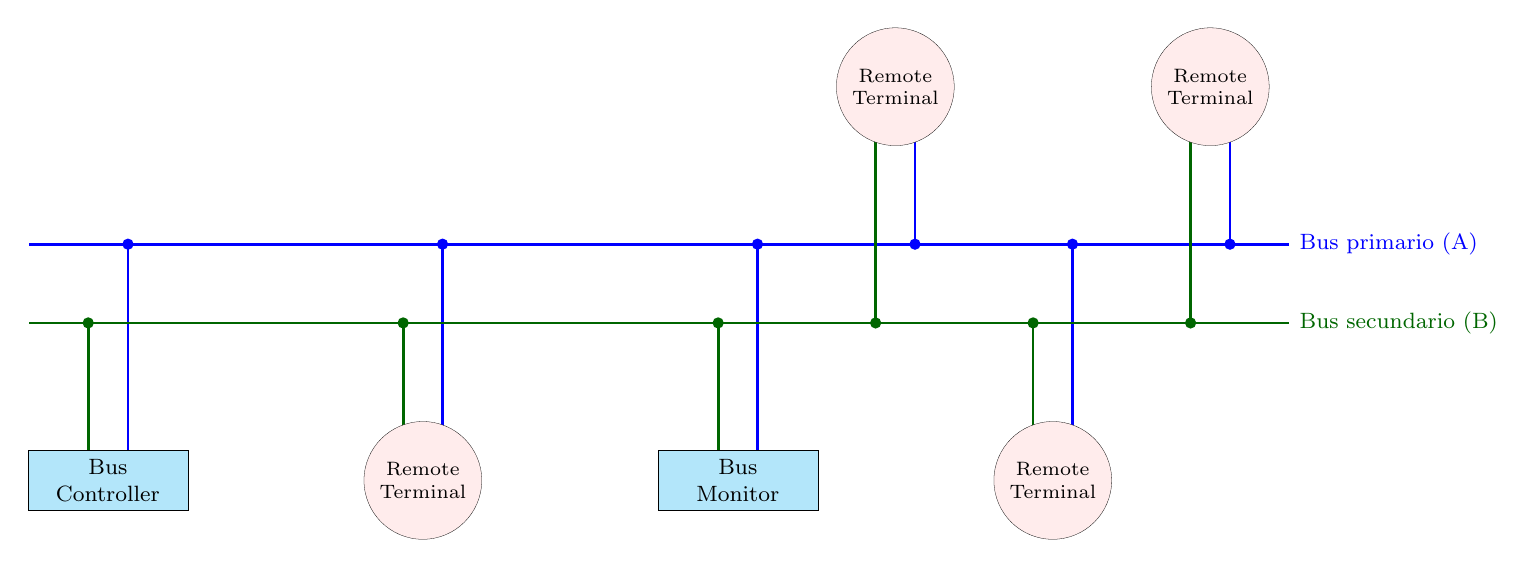
\begin{tikzpicture}[ node distance=1cm,
             conexion/.style = { circle, 
                                                 minimum size = 3 ,
                                              draw,
												fill ,
											inner sep=0 ,
                                                },
				font = \footnotesize , 
               Transmisor/.style ={ fill=cyan!30 , 
                          draw,
                          line width= 0.1 , 
						text width=1.8cm,
						align = center
                        } ,
               Receptor/.style ={  font = \scriptsize, 
						circle ,
                          fill=pink!30 , 
                          draw,
%						text width=1.2cm,
						align = center ,
                          line width= 0.1 , 
                        } ,
                     ]

% grilla
%  \draw[ green!50!black] (0,0) grid (20,10) ;

% Bus primario
\draw[line width=1, blue]  (0 , 4) -- +(16 , 0) node[above, right] {Bus primario (A)}
                       (1.255 , 4 ) node[conexion ] {} -- +(0 , -3) 
                       (5.25 , 4 ) node[conexion ] {} -- +(0 , -3) 
                       (9.25 , 4 ) node[conexion ] {} -- +(0 , -3)
                        (11.25 , 4 ) node[conexion ] {} -- +(0 , 2)
                       (13.25 , 4 ) node[conexion ] {} -- +(0 , -3) 
                       (15.25 , 4 ) node[conexion ] {} -- +(0 , 2) 
;

% Bus secundario
\draw[line width=1, green!40!black]  (0 , 3) -- +(16 , 0) node[above, right] {Bus secundario (B)} 
                       (0.75 , 3 ) node[conexion ] {} -- +(0 , -2) 
                       (4.75 , 3 ) node[conexion ] {} -- +(0 , -2) 
                       (8.75 , 3 ) node[conexion ] {} -- +(0 , -2) 
                      (10.75 , 3 ) node[conexion ] {} -- +(0 ,  3)
                      (12.75 , 3 ) node[conexion ] {} -- +(0 ,  -2)
                      (14.75 , 3 ) node[conexion ] {} -- +(0 ,  3)
;

% Elementos del bus
\draw ( 1 ,1 ) node[Transmisor] (BS) {Bus \\Controller} 
            +( 4 , 0 ) node[Receptor] (RT1) {Remote \\Terminal} 
            +( 8 , 0 ) node[Transmisor] (BM) {Bus \\ Monitor} 
            +( 10 , 5 ) node[Receptor] (RT2) {Remote \\Terminal} 
            +( 12 , 0 ) node[Receptor] (RT3) {Remote \\Terminal} 
            +( 14 , 5 ) node[Receptor] (RT4) {Remote \\Terminal} 
;





\end{tikzpicture}
%}
  \caption{Arquitectura de MIL-STD-1553, adaptado de \protect\cite{MIL-1553-tutorial}}
  \label{fig:01.MIL.1553.componentes}
\end{figure}



\subsubsection{STANAG 3838}
\label{sec:01.02.STANAG.3838}

\begin{myboxAmarillo}{STANAG}
  El STANdardization AGreement (STANAG, Acuerdo de Normalización) de
  la OTAN (Organización del Tratado del Atlántico Norte) definen
  procesos, procedimientos, términos y condiciones de equipamiento o
  procedimientos y técnicas militares comunes entre los países
  miembros de dicha alianza.
\end{myboxAmarillo}


El protocolo MIL-STD-1553 
fué adoptado por la OTAN como STANAG 3838 empleando el método de transmisión bidireccional por una sola línea  de 16 bits. Es redundante porque emplea dos buses y dos controladores de bus. Su velocidad de transmisión es de 1Mb/seg.

\subsubsection{STANAG 3910 }
\label{sec:01.02.STANAG3910 }

Es un protocolo de bus de alta velocidad de 16 bit bajo STANAG 3838 o control equivalente mediante fibra óptica. Se emplea principalmente para uso en sistemas de aviónica y que permite aumentar un bus de datos STANAG 3838 o MIL-STD-1553B de 1 Mb/seg a un bus de datos de alta velocidad de 20 Mb/seg denominado canal HS mediante, entre otros elementos, el uso de fibra óptica..

El bus STANAG 3838 / MIL-STD-1553B en una implementación de STANAG 3910 se denomina canal de baja velocidad (LS) y emplea canales de cobre. 

Ambos canales o cualquiera de ellos pueden tener redundancia múltiple y emplear medios eléctricos u ópticos.

\subsubsection{CSDB y ASCB}
\label{sec:01.02.CSDB+ASCB}

Son protocolos patentados de Collins (CSDB) y Honeywell (ASCB). 
Estos sistemas se utilizan a menudo en pequeñas empresas y aviones privados de aviación general. 

CSDB es un bus unidireccional que permite la conexión de hasta diez receptores y un transmisor. El estándar admite velocidades de datos de 12,5 kbps y 50 kbps. 

ASCB es un bus bidireccional controlado centralmente. Una configuración básica comprende un controlador de bus único y dos buses aislados, cada uno de los cuales puede admitir hasta 48 dispositivos.

\subsubsection{FDDI}
\label{sec:01.02.FDDI}

La Interfaz de Datos Distribuidos por Fibra (FDDI) fue desarrollada originalmente por Boeing para su uso en el avión Boeing 777. 

FDDI es una red de área local (LAN) basada en una topología de anillo de token dual. Los datos en cada anillo fluyen en direcciones opuestas. La velocidad de datos es de 100 Mbps y los datos se codifican en cuadros. 
CDDI (Interfaz de Datos Distribuidos de Cobre) y SDDI (Interfaz de Datos Distribuidos de Par Trenzado Blindado) son estándares de bus de red similares empleando como medios físicos cables de cobre y par trenzado blindado. 
El formato de datos es NRZI, formato de datos similar a NRZ, pero en el cual un cambio en el nivel de voltaje de línea indica un 1 lógico y ningún cambio indica un 0 lógico. 
%Por razones de costo y para reducir el número y la complejidad de los estándares de red utilizados en sus aeronaves avión, Boeing ahora planea reemplazar el sistema en el 777 con un ethernet de cobre de 10 Mbps menos costoso.
